\documentclass{beamer}
\usetheme{Juelich}

\title{Quantum Boltzmann Machines}
\subtitle{Applications in Quantitative Finance}
\author{Cameron Perot}
\institute{JSC}
\date{\today}
\titlegraphic{\includegraphics%
    [height=0.45\paperheight]{placeholder}
}

% packages
\usepackage{adjustbox}
\usepackage{amssymb}
\usepackage{amsmath}
\usepackage{float}
\usepackage{graphicx}
\usepackage{braket}
\usepackage{multirow}
\usepackage{bbm}
\usepackage{mathtools}
\usepackage{booktabs}

\graphicspath{ {../../../results/plots/}{../../images/} }

% new commands
% Misc. commands
\newcommand{\CNOT}[2]{\text{C}_{#1}\text{NOT}_{#2}}
\newcommand{\SWAP}{\text{SWAP}}
\newcommand{\CZ}{\text{CZ}}
\newcommand{\tr}{\text{tr}}
\newcommand{\frt}{\frac{1}{\sqrt{2}}}
\newcommand{\Z}{\mathbb{Z}}
\newcommand{\R}{\mathbb{R}}
\newcommand{\N}{\mathbb{N}}
\newcommand{\mat}[1]{\mathbf{#1}}
\newcommand{\binset}{\{0,1\}}
\newcommand{\spause}{s_{\text{pause}}}
\newcommand{\tpause}{t_{\text{pause}}}
\newcommand{\Deltapause}{\Delta_{\text{pause}}}
\newcommand{\Deltaquench}{\Delta_{\text{quench}}}
\newcommand{\alphaquench}{\alpha_{\text{quench}}}
\renewcommand{\vec}[1]{\mathbf{#1}}
\newcommand{\basistwo}{\{\ket{00}, \ket{01}, \ket{10}, \ket{11}\}}
\DeclarePairedDelimiter{\norm}{\lVert}{\rVert}
\DeclarePairedDelimiter{\abs}{\lvert}{\rvert}

% Identity operator (on K^2)
\newcommand{\idtwo}{
    \begin{bmatrix}
        1 & 0 \\
        0 & 1
    \end{bmatrix}
}

% Hadamard operator
\newcommand{\Hgate}{
    \frac{1}{\sqrt{2}} \begin{bmatrix}
        1 & 1 \\
        1 & -1
    \end{bmatrix}
}

% T gate
\newcommand{\Tgate}{
    \begin{bmatrix}
        1 & 0 \\
        0 & e^{i \pi / 4}
    \end{bmatrix}
}

% T gate dag
\newcommand{\Tgatedag}{
    \begin{bmatrix}
        1 & 0 \\
        0 & e^{-i \pi / 4}
    \end{bmatrix}
}

% R_X
\newcommand{\RXGate}[1]{
    \begin{bmatrix}
        \cos\frac{#1}{2} & -i\sin\frac{#1}{2} \\
        -i\sin\frac{#1}{2} & \cos\frac{#1}{2}
    \end{bmatrix}
}

% R_Y
\newcommand{\RYGate}[1]{
    \begin{bmatrix}
        \cos\frac{#1}{2} & -\sin\frac{#1}{2} \\
        \sin\frac{#1}{2} & \cos\frac{#1}{2}
    \end{bmatrix}
}

% R_Z
\newcommand{\RZGate}[1]{
    \begin{bmatrix}
        e^{-i{#1}/2} & 0 \\
        0 & e^{i{#1}/2}
    \end{bmatrix}
}

% Pauli X operator
\newcommand{\XGate}{
    \begin{bmatrix}
        0 & 1 \\
        1 & 0
    \end{bmatrix}
}

% Pauli Y operator
\newcommand{\YGate}{
    \begin{bmatrix}
        0 & -i \\
        i & 0
    \end{bmatrix}
}

% Pauli Z operator
\newcommand{\ZGate}{
    \begin{bmatrix}
        1 & 0 \\
        0 & -1
    \end{bmatrix}
}

% The |0⟩ state in vector form
\newcommand{\zerostate}{
    \begin{bmatrix}
        1 \\
        0
    \end{bmatrix}
}

% The |1⟩ state in vector form
\newcommand{\onestate}{
    \begin{bmatrix}
        0 \\
        1
    \end{bmatrix}
}

% The |-⟩ state in vector form
\newcommand{\minusstatey}{
    \frac{1}{\sqrt{2}}
    \begin{bmatrix}
        1 \\
        -i
    \end{bmatrix}
}

% The |+⟩ state in vector form
\newcommand{\plusstatey}{
    \frac{1}{\sqrt{2}}
    \begin{bmatrix}
        1 \\
        i
    \end{bmatrix}
}

% The |-'⟩ state in vector form
\newcommand{\minusstate}{
    \frac{1}{\sqrt{2}}
    \begin{bmatrix}
        1 \\
        -1
    \end{bmatrix}
}

% The |+'⟩ state in vector form
\newcommand{\plusstate}{
    \frac{1}{\sqrt{2}}
    \begin{bmatrix}
        1 \\
        1
    \end{bmatrix}
}


\begin{document}
%----------------------------------------------------------------------------------------
% Title Page
%----------------------------------------------------------------------------------------

\maketitle

%----------------------------------------------------------------------------------------
% Table of Contents
%----------------------------------------------------------------------------------------

\begin{frame}
    \frametitle{Overview}
    \tableofcontents
\end{frame}

%----------------------------------------------------------------------------------------
% Data Analysis
%----------------------------------------------------------------------------------------

\section{Data Analysis and Preprocessing}

\subsection{Data Analysis}
\begin{frame}
    \frametitle{Foreign Exchange Log Returns Data Set}
    Data set consisted of the daily log returns for the time period 1999-01-01 through 2019-12-31 of the following major currency pairs
    \begin{itemize}
        \item EURUSD - Euro € / U.S. Dollar \$
        \item GBPUSD - British Pound Sterling £ / U.S. Dollar \$
        \item USDCAD - U.S. Dollar \$ / Canadian Dollar \$
        \item USDJPY - U.S. Dollar \$ / Japanese Yen ¥
    \end{itemize}
    obtained from Dukascopy historical data feed~\cite{dukascopy}.
    Log return of currency \( x \) on a particular day given by
    \begin{align}
        \tilde{r}
            = \log\bigg( \frac{x_\text{close}}{x_\text{open}} \bigg)
    \end{align}
\end{frame}

\begin{frame}
    \frametitle{Histograms}
    \begin{figure}
        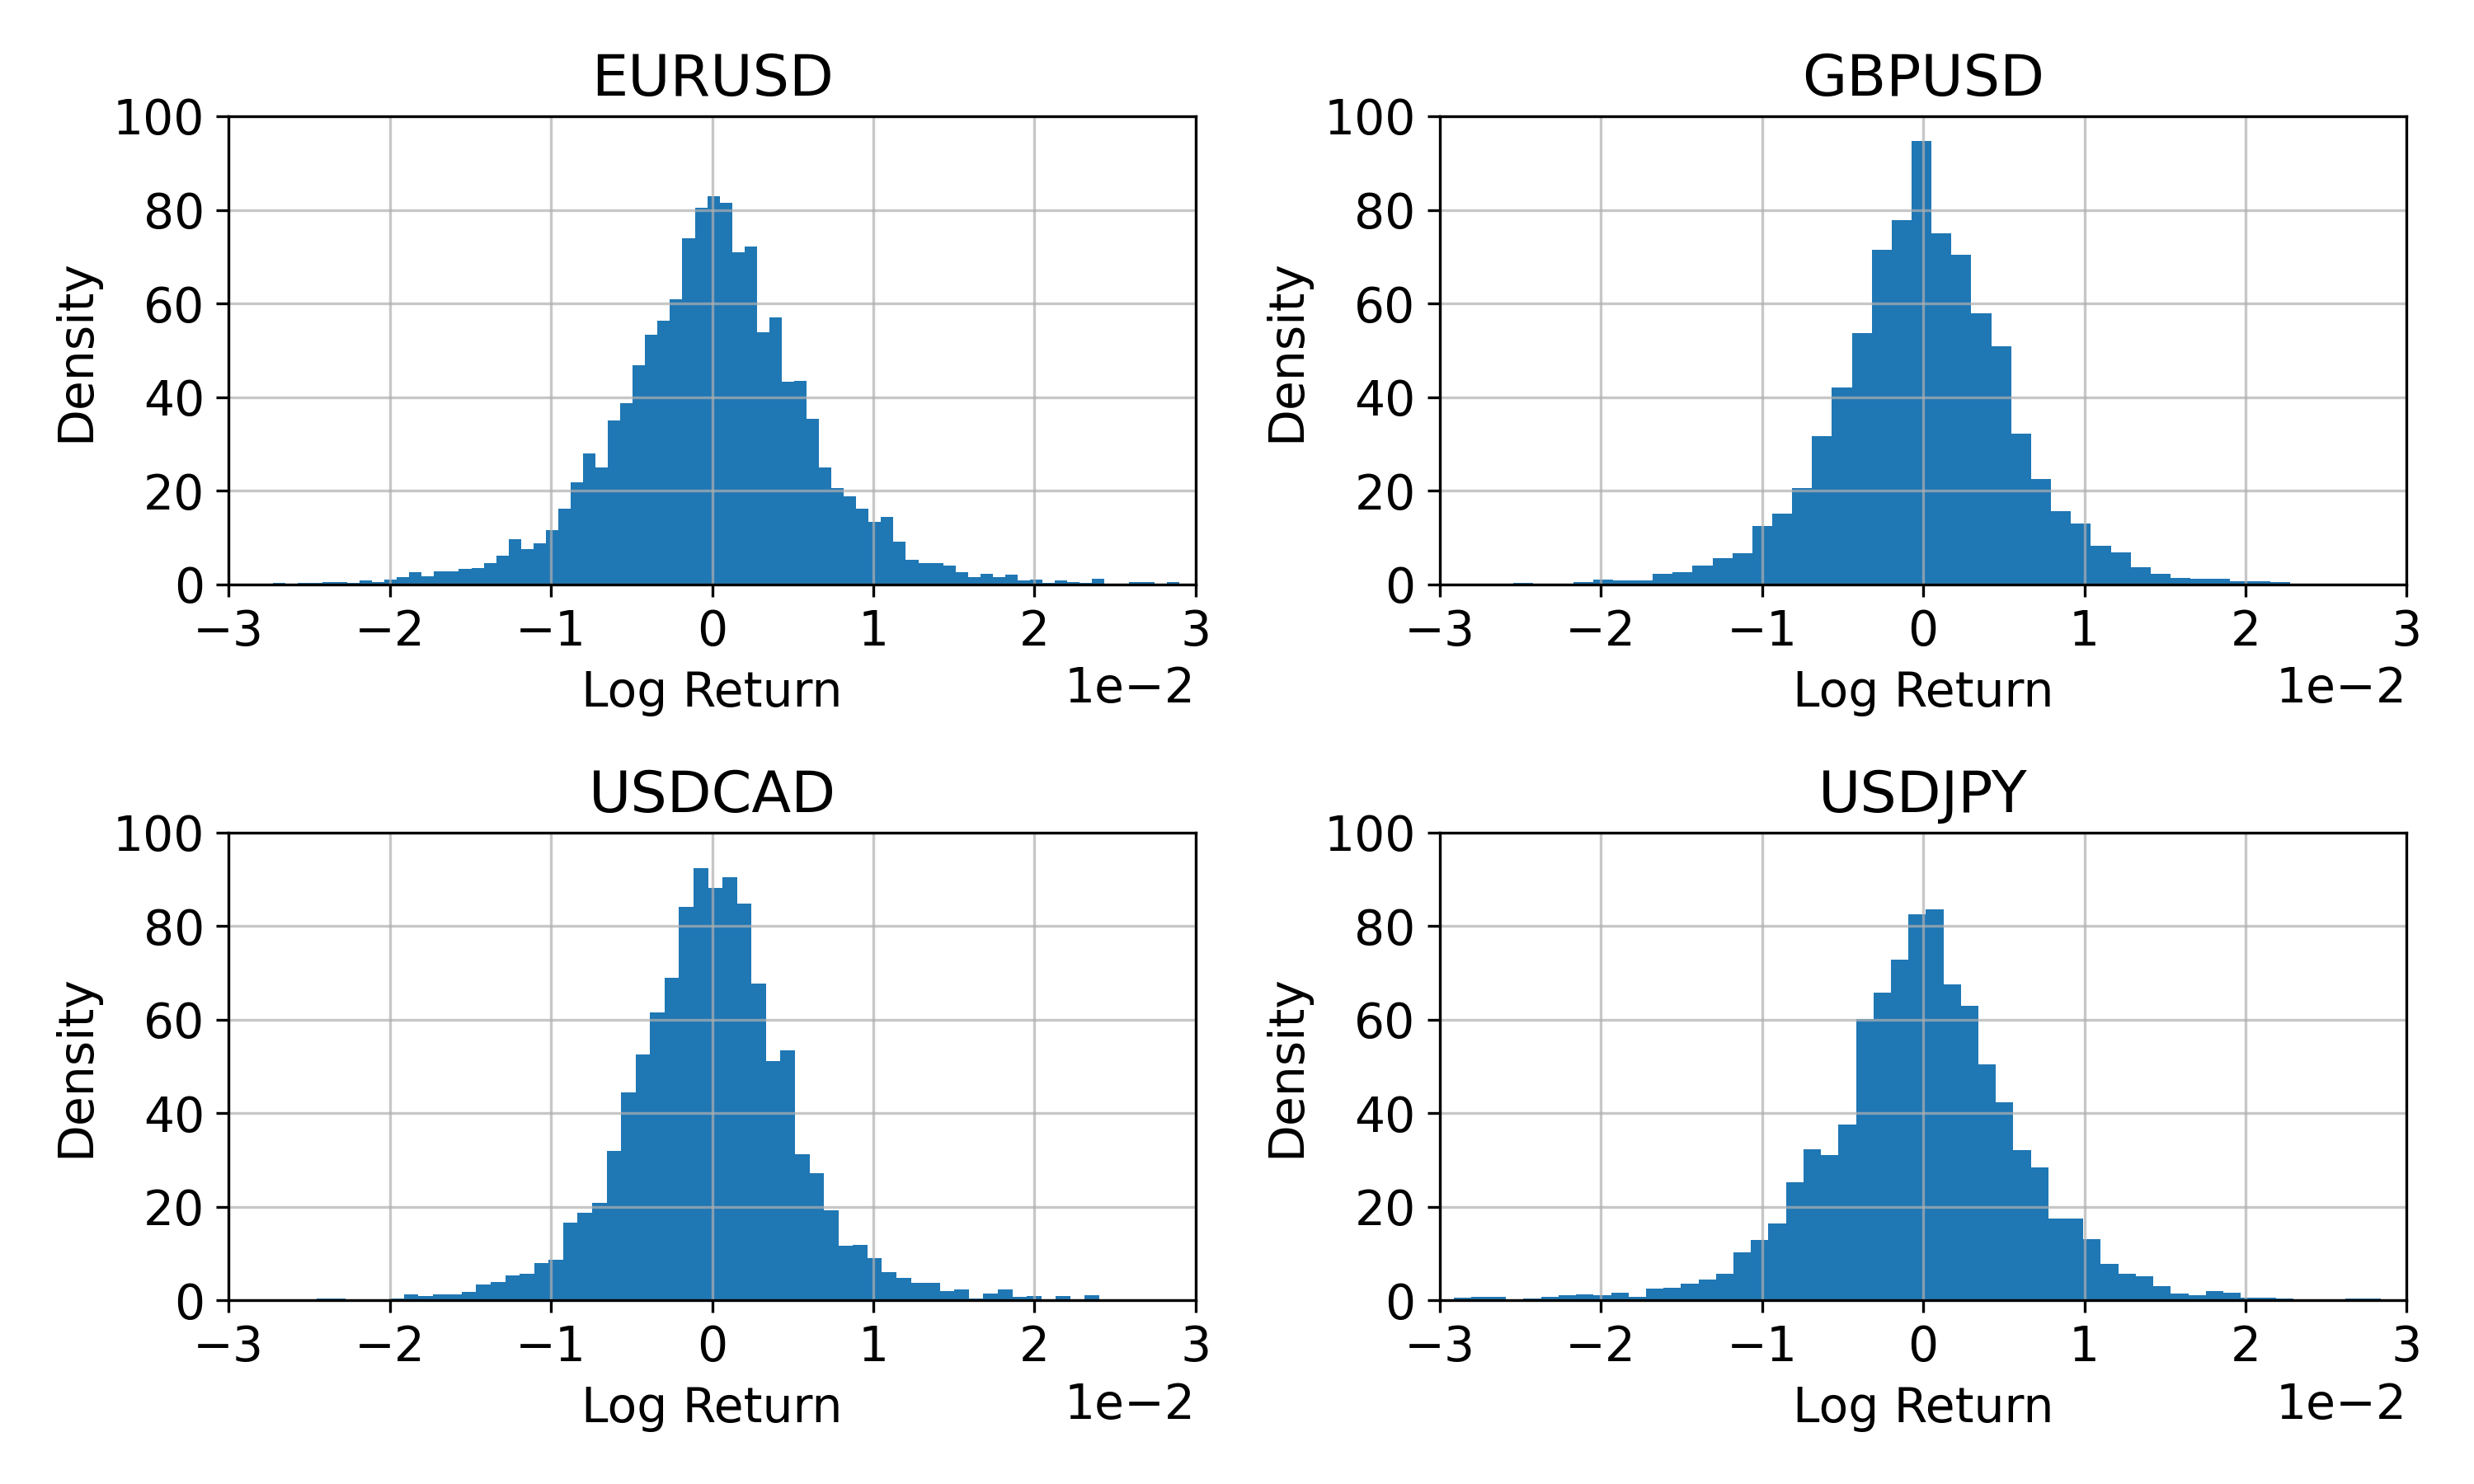
\includegraphics[width=1\linewidth]{data_analysis/histograms.png}
    \end{figure}
\end{frame}

\begin{frame}
    \frametitle{Violin/Box Plot}
    \begin{figure}
        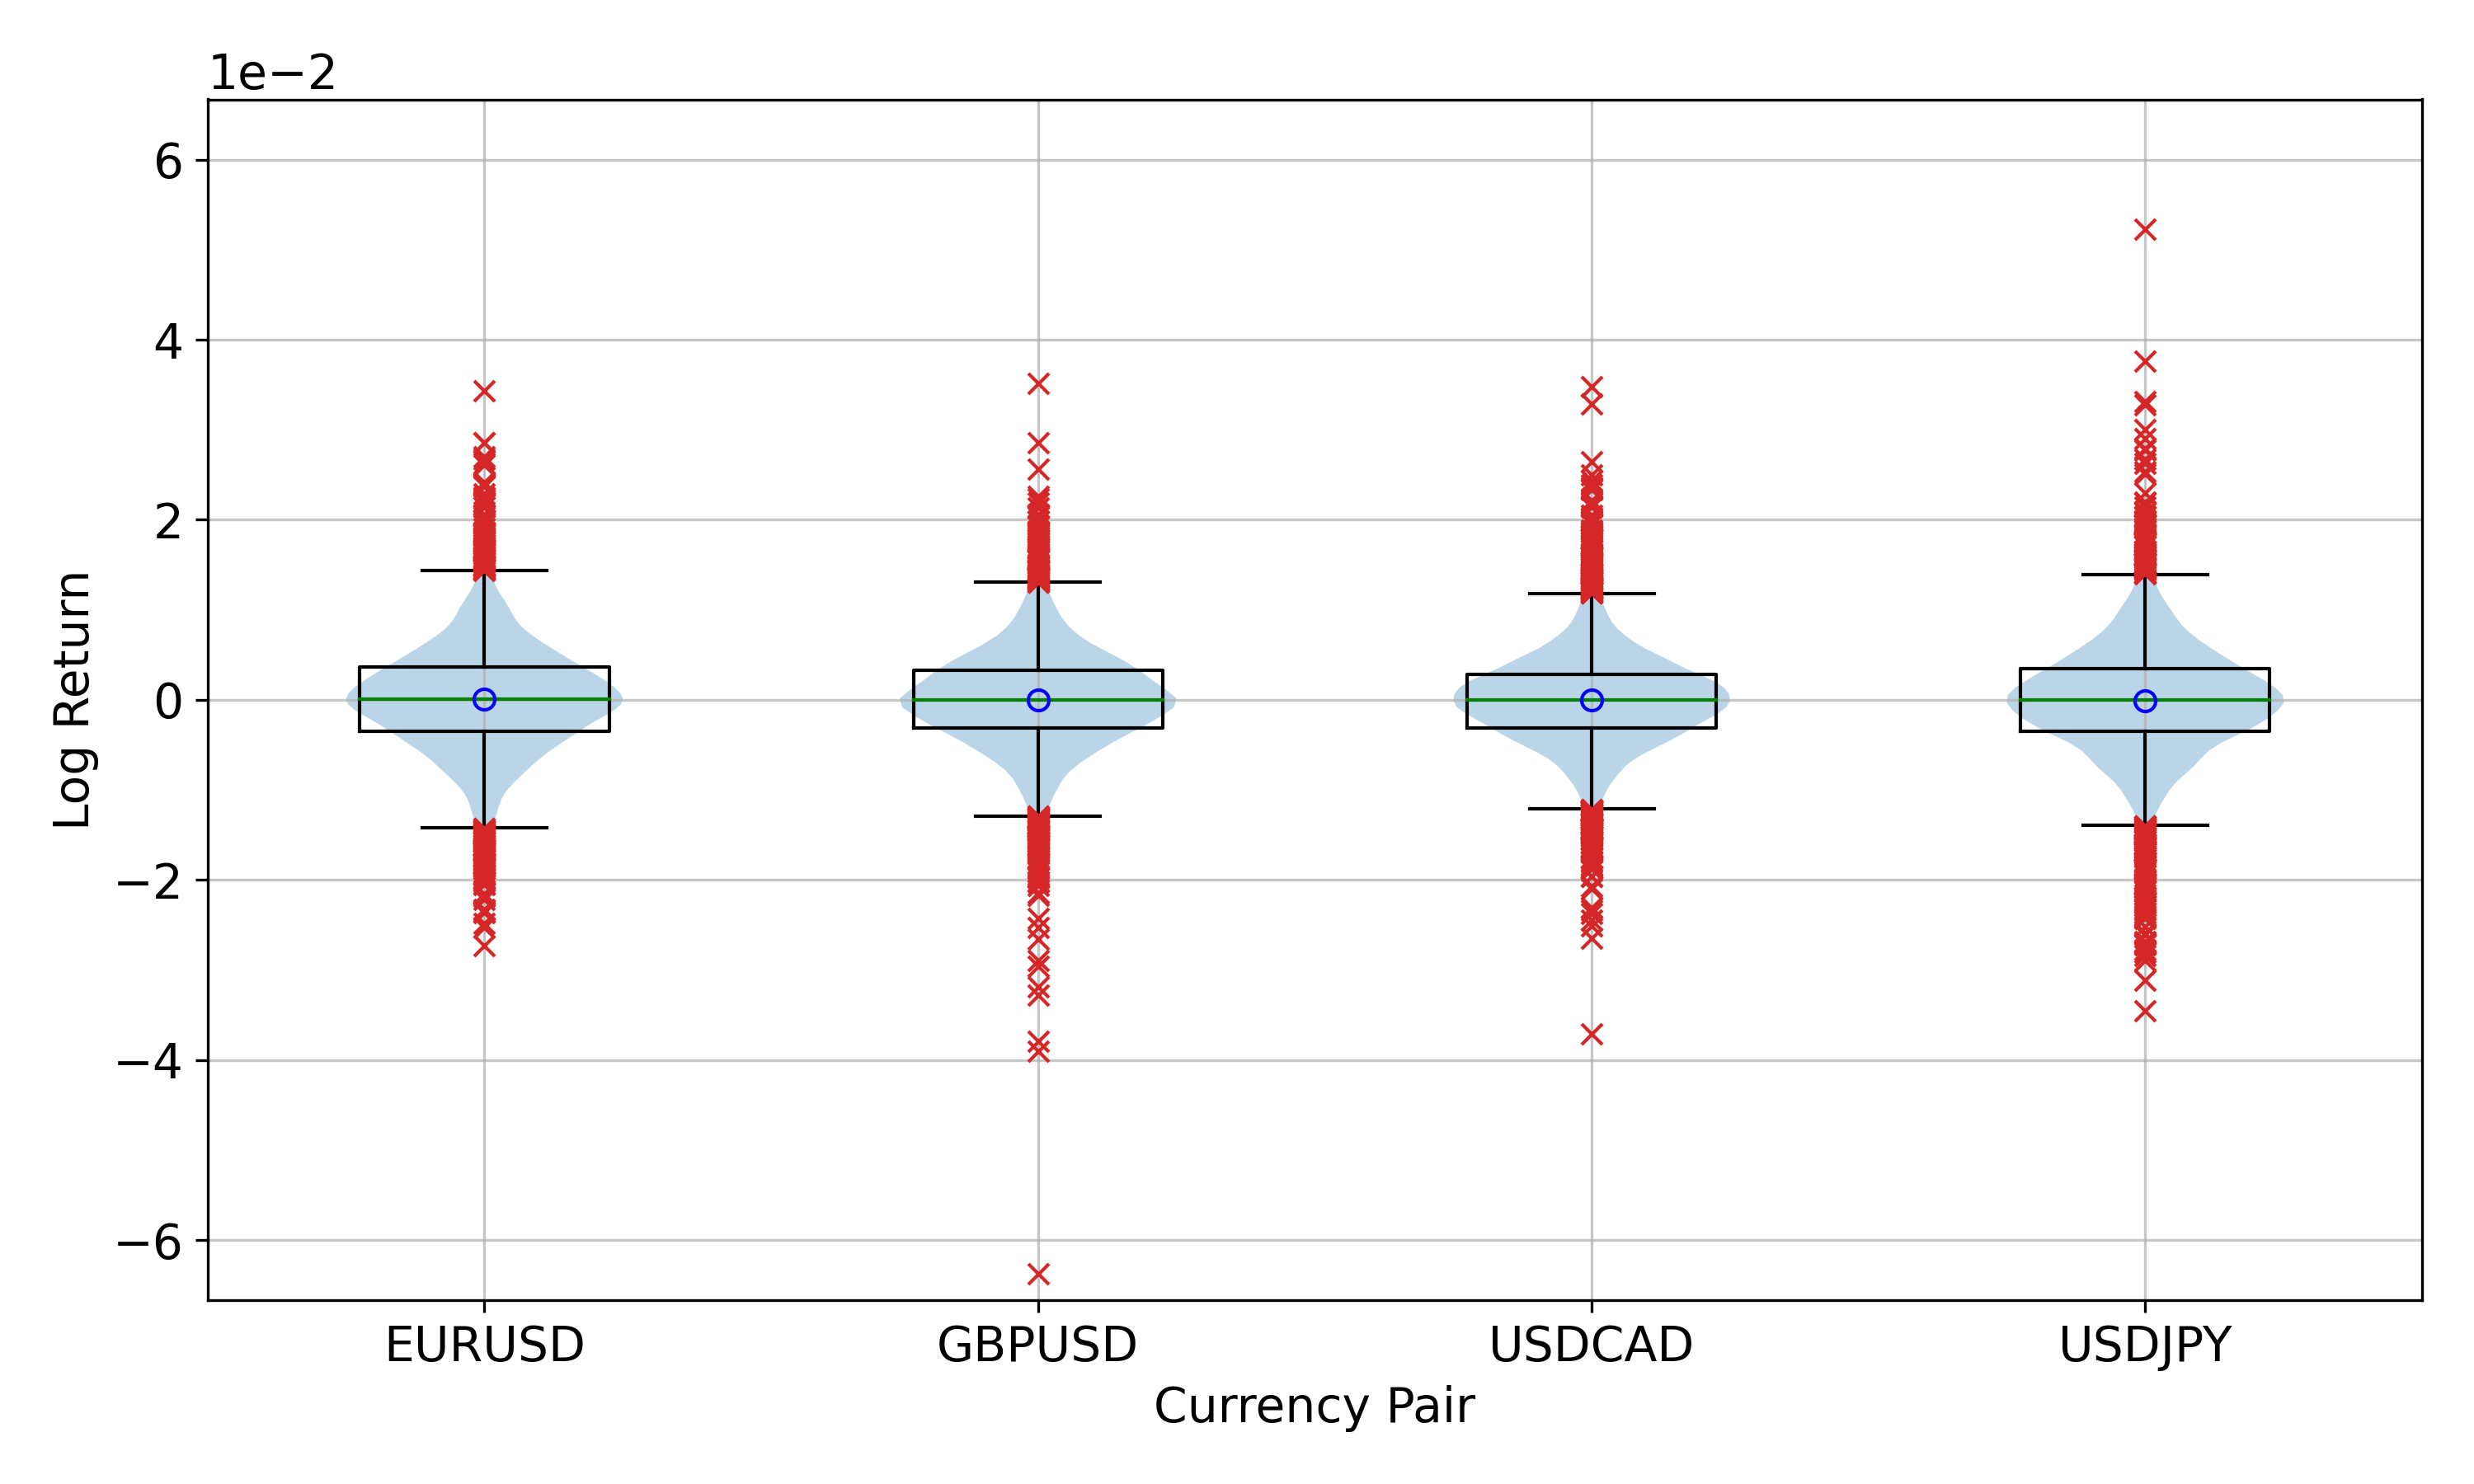
\includegraphics[width=1\linewidth]{data_analysis/violin.png}
    \end{figure}
\end{frame}

\begin{frame}
    \frametitle{Scatter Plots}
    \begin{figure}
        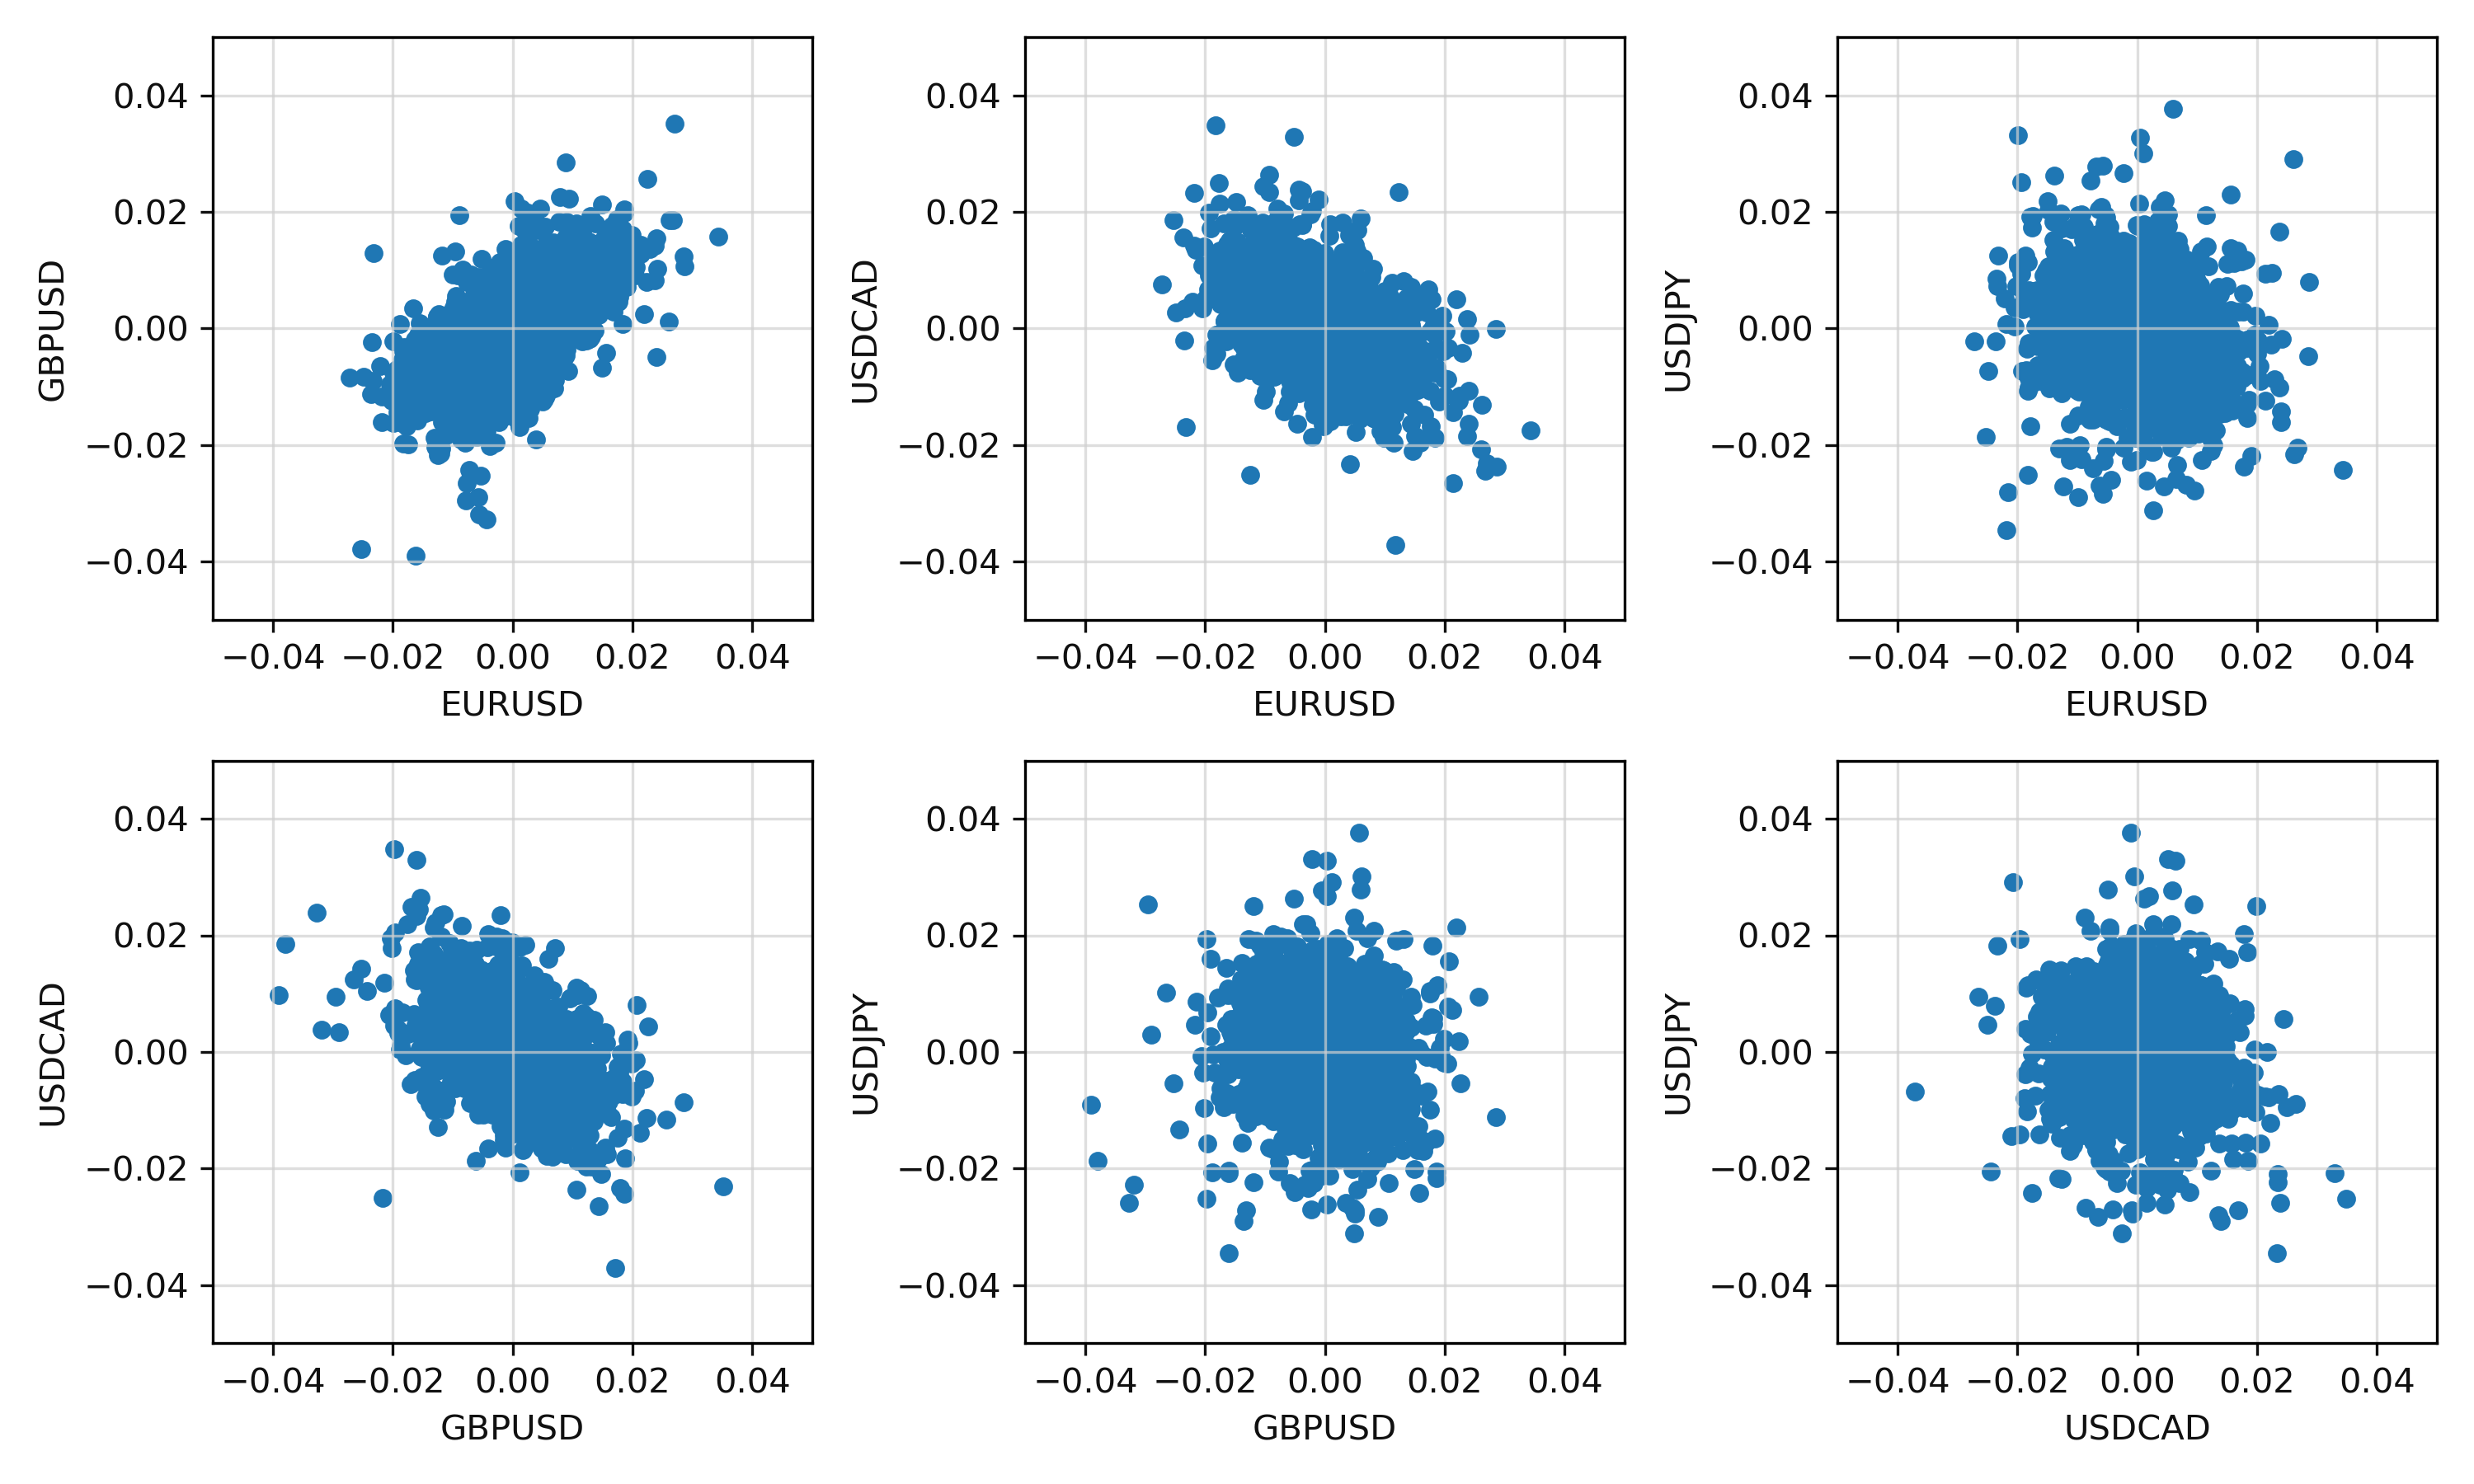
\includegraphics[width=1\linewidth]{data_analysis/scatters.png}
    \end{figure}
\end{frame}

\subsection{Data Preprocessing}
\begin{frame}
    \frametitle{Discretization to Bit Vectors}
    Each currency pair's log returns linearly discretized into \( 2^{n_\text{bits}} \) states.
    Index \( i \) denotes the currency pair, and index \( j \) denotes the sample.
    \begin{align}
        x_{ij}' = \bigg\lfloor \frac{x_{ij} - \min_k \{x_{ik}\}}{\max_k \{x_{ik}\} - \min_k \{x_{ik}\}} \cdot (2^{n_\text{bits}} - 1) \bigg\rceil
    \end{align}
    The \( j \)th training sample is given by
    \begin{align}
        \begin{bmatrix}
            \text{bitvector}(x_{1j}') \\
            \text{bitvector}(x_{2j}') \\
            \text{bitvector}(x_{3j}') \\
            \text{bitvector}(x_{4j}') \\
        \end{bmatrix}
        \in \binset^{4\cdot n_\text{bits}}
    \end{align}

\end{frame}

\begin{frame}
    \frametitle{Preprocessing Outlier Transformation}
    \begin{figure}
        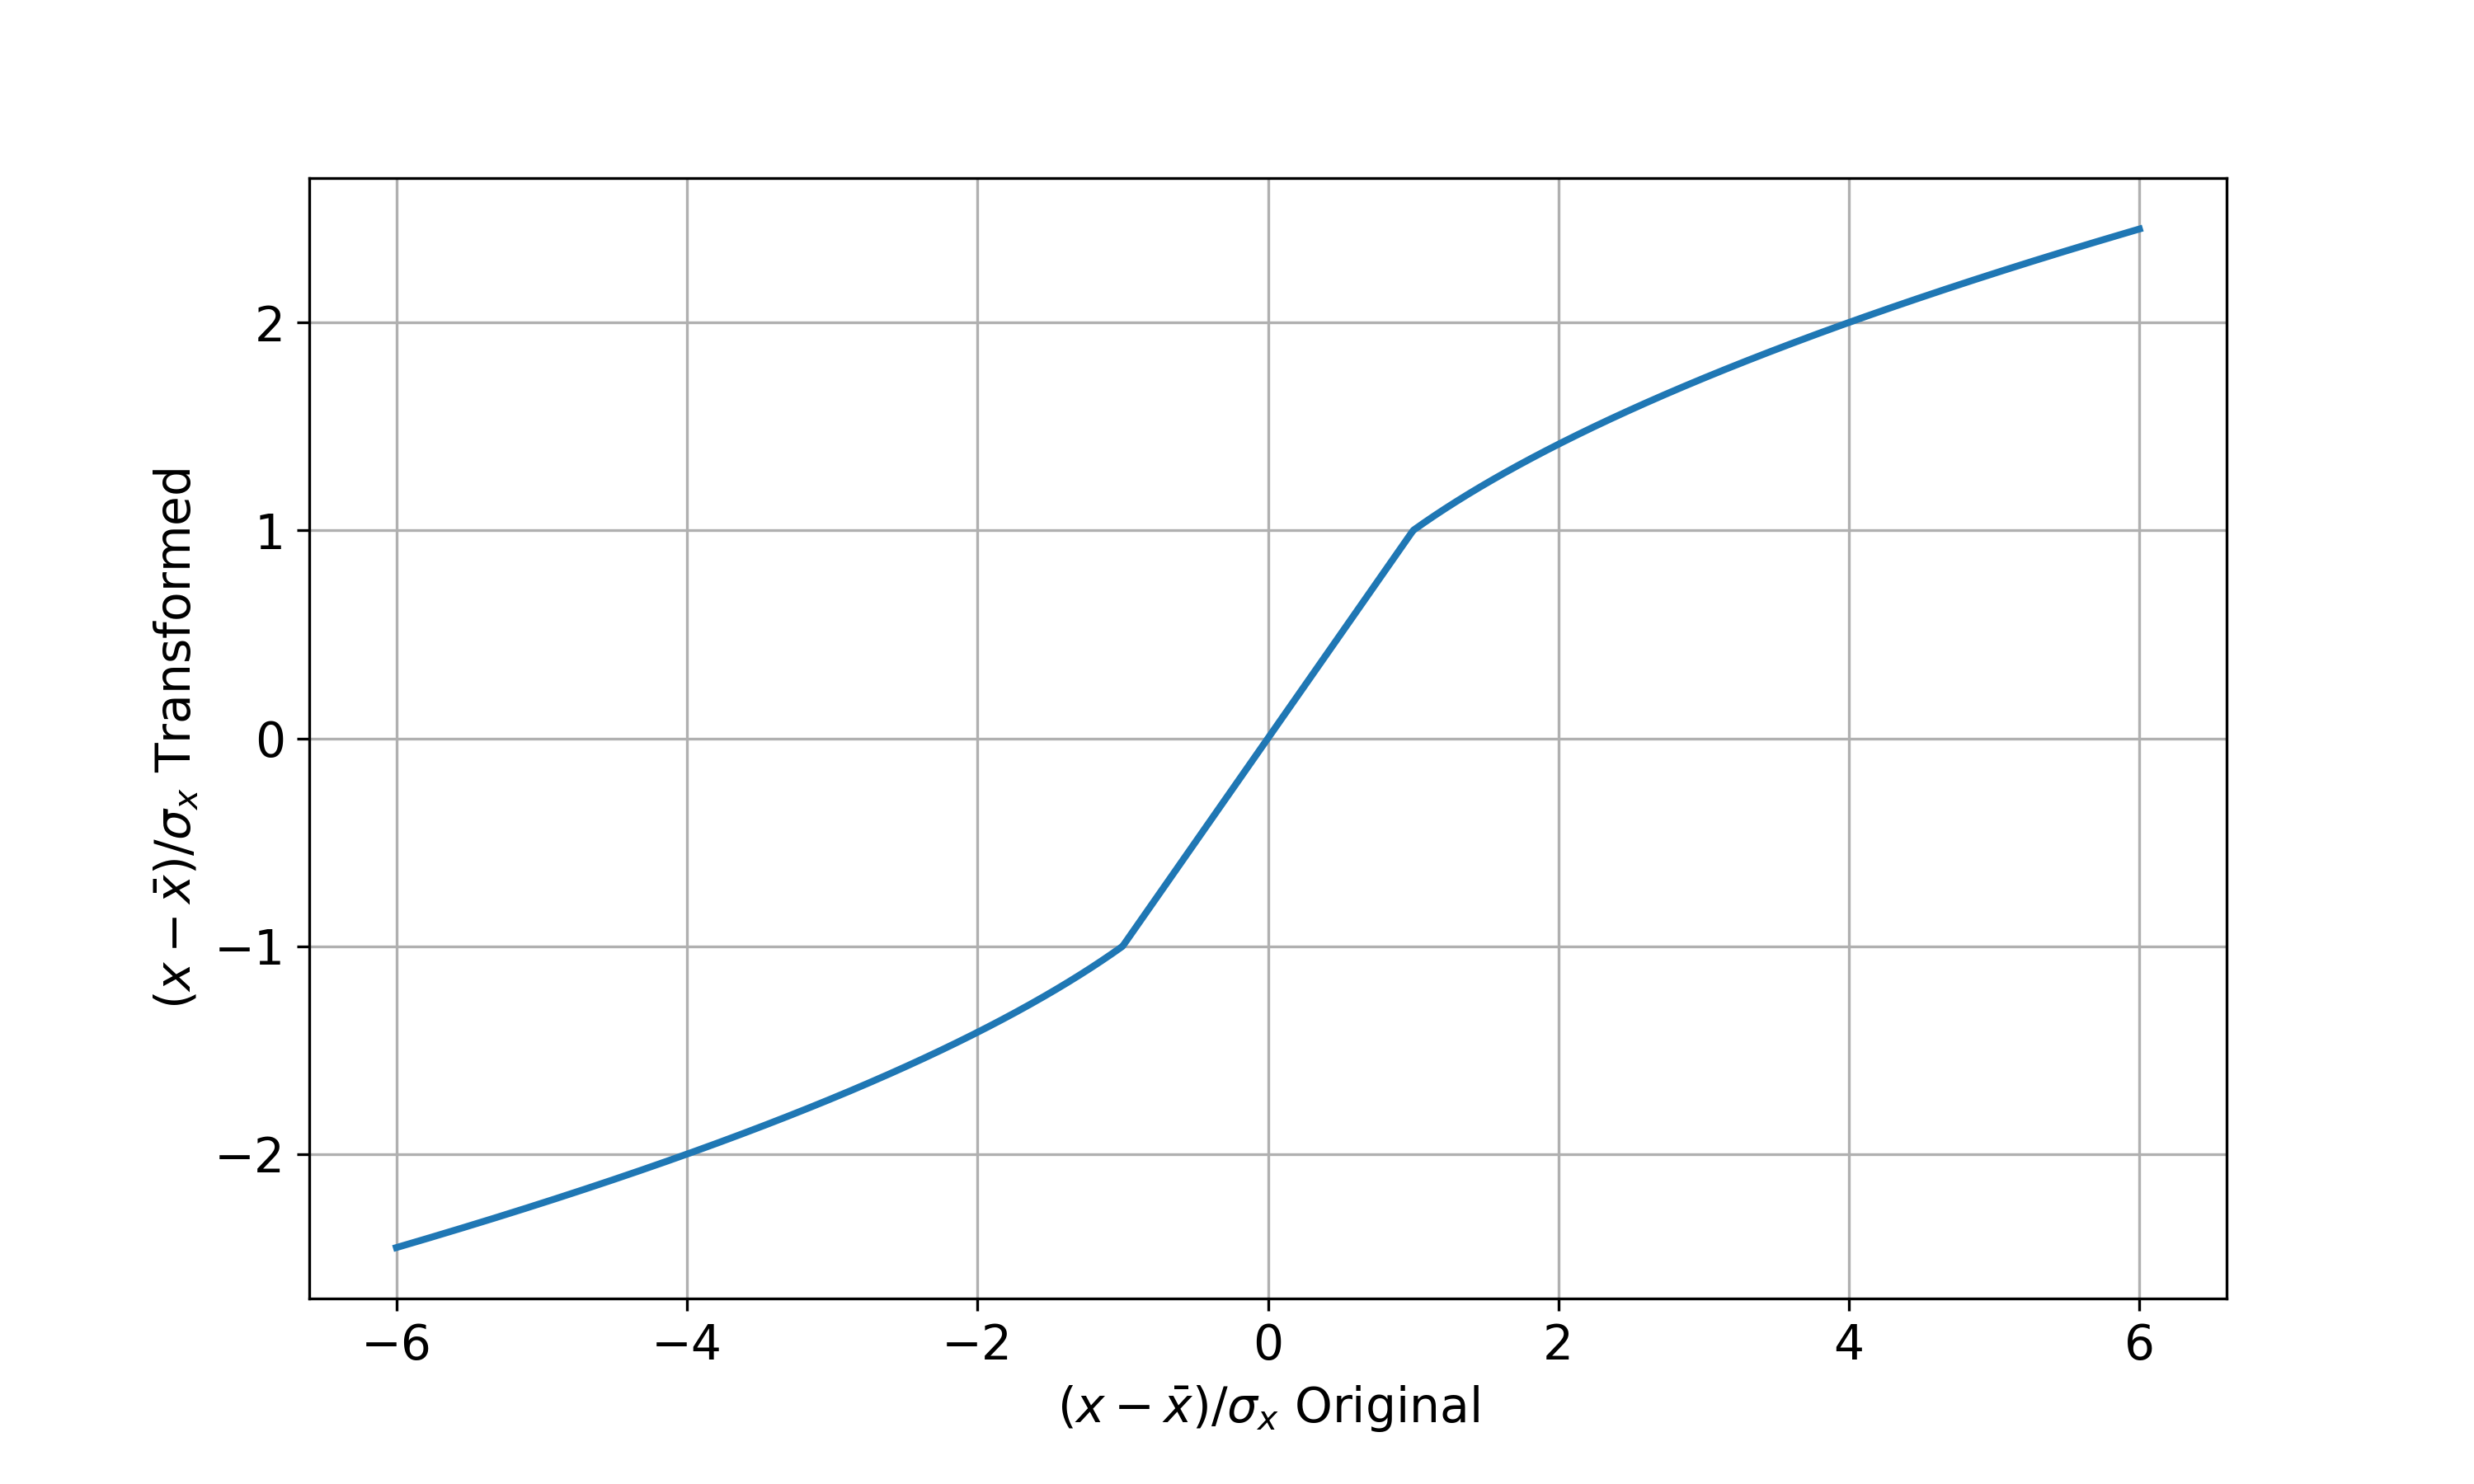
\includegraphics[width=1\linewidth]{data_analysis/data_transformation.png}
    \end{figure}
\end{frame}

\begin{frame}
    \frametitle{Transformed Histograms}
    \begin{figure}
        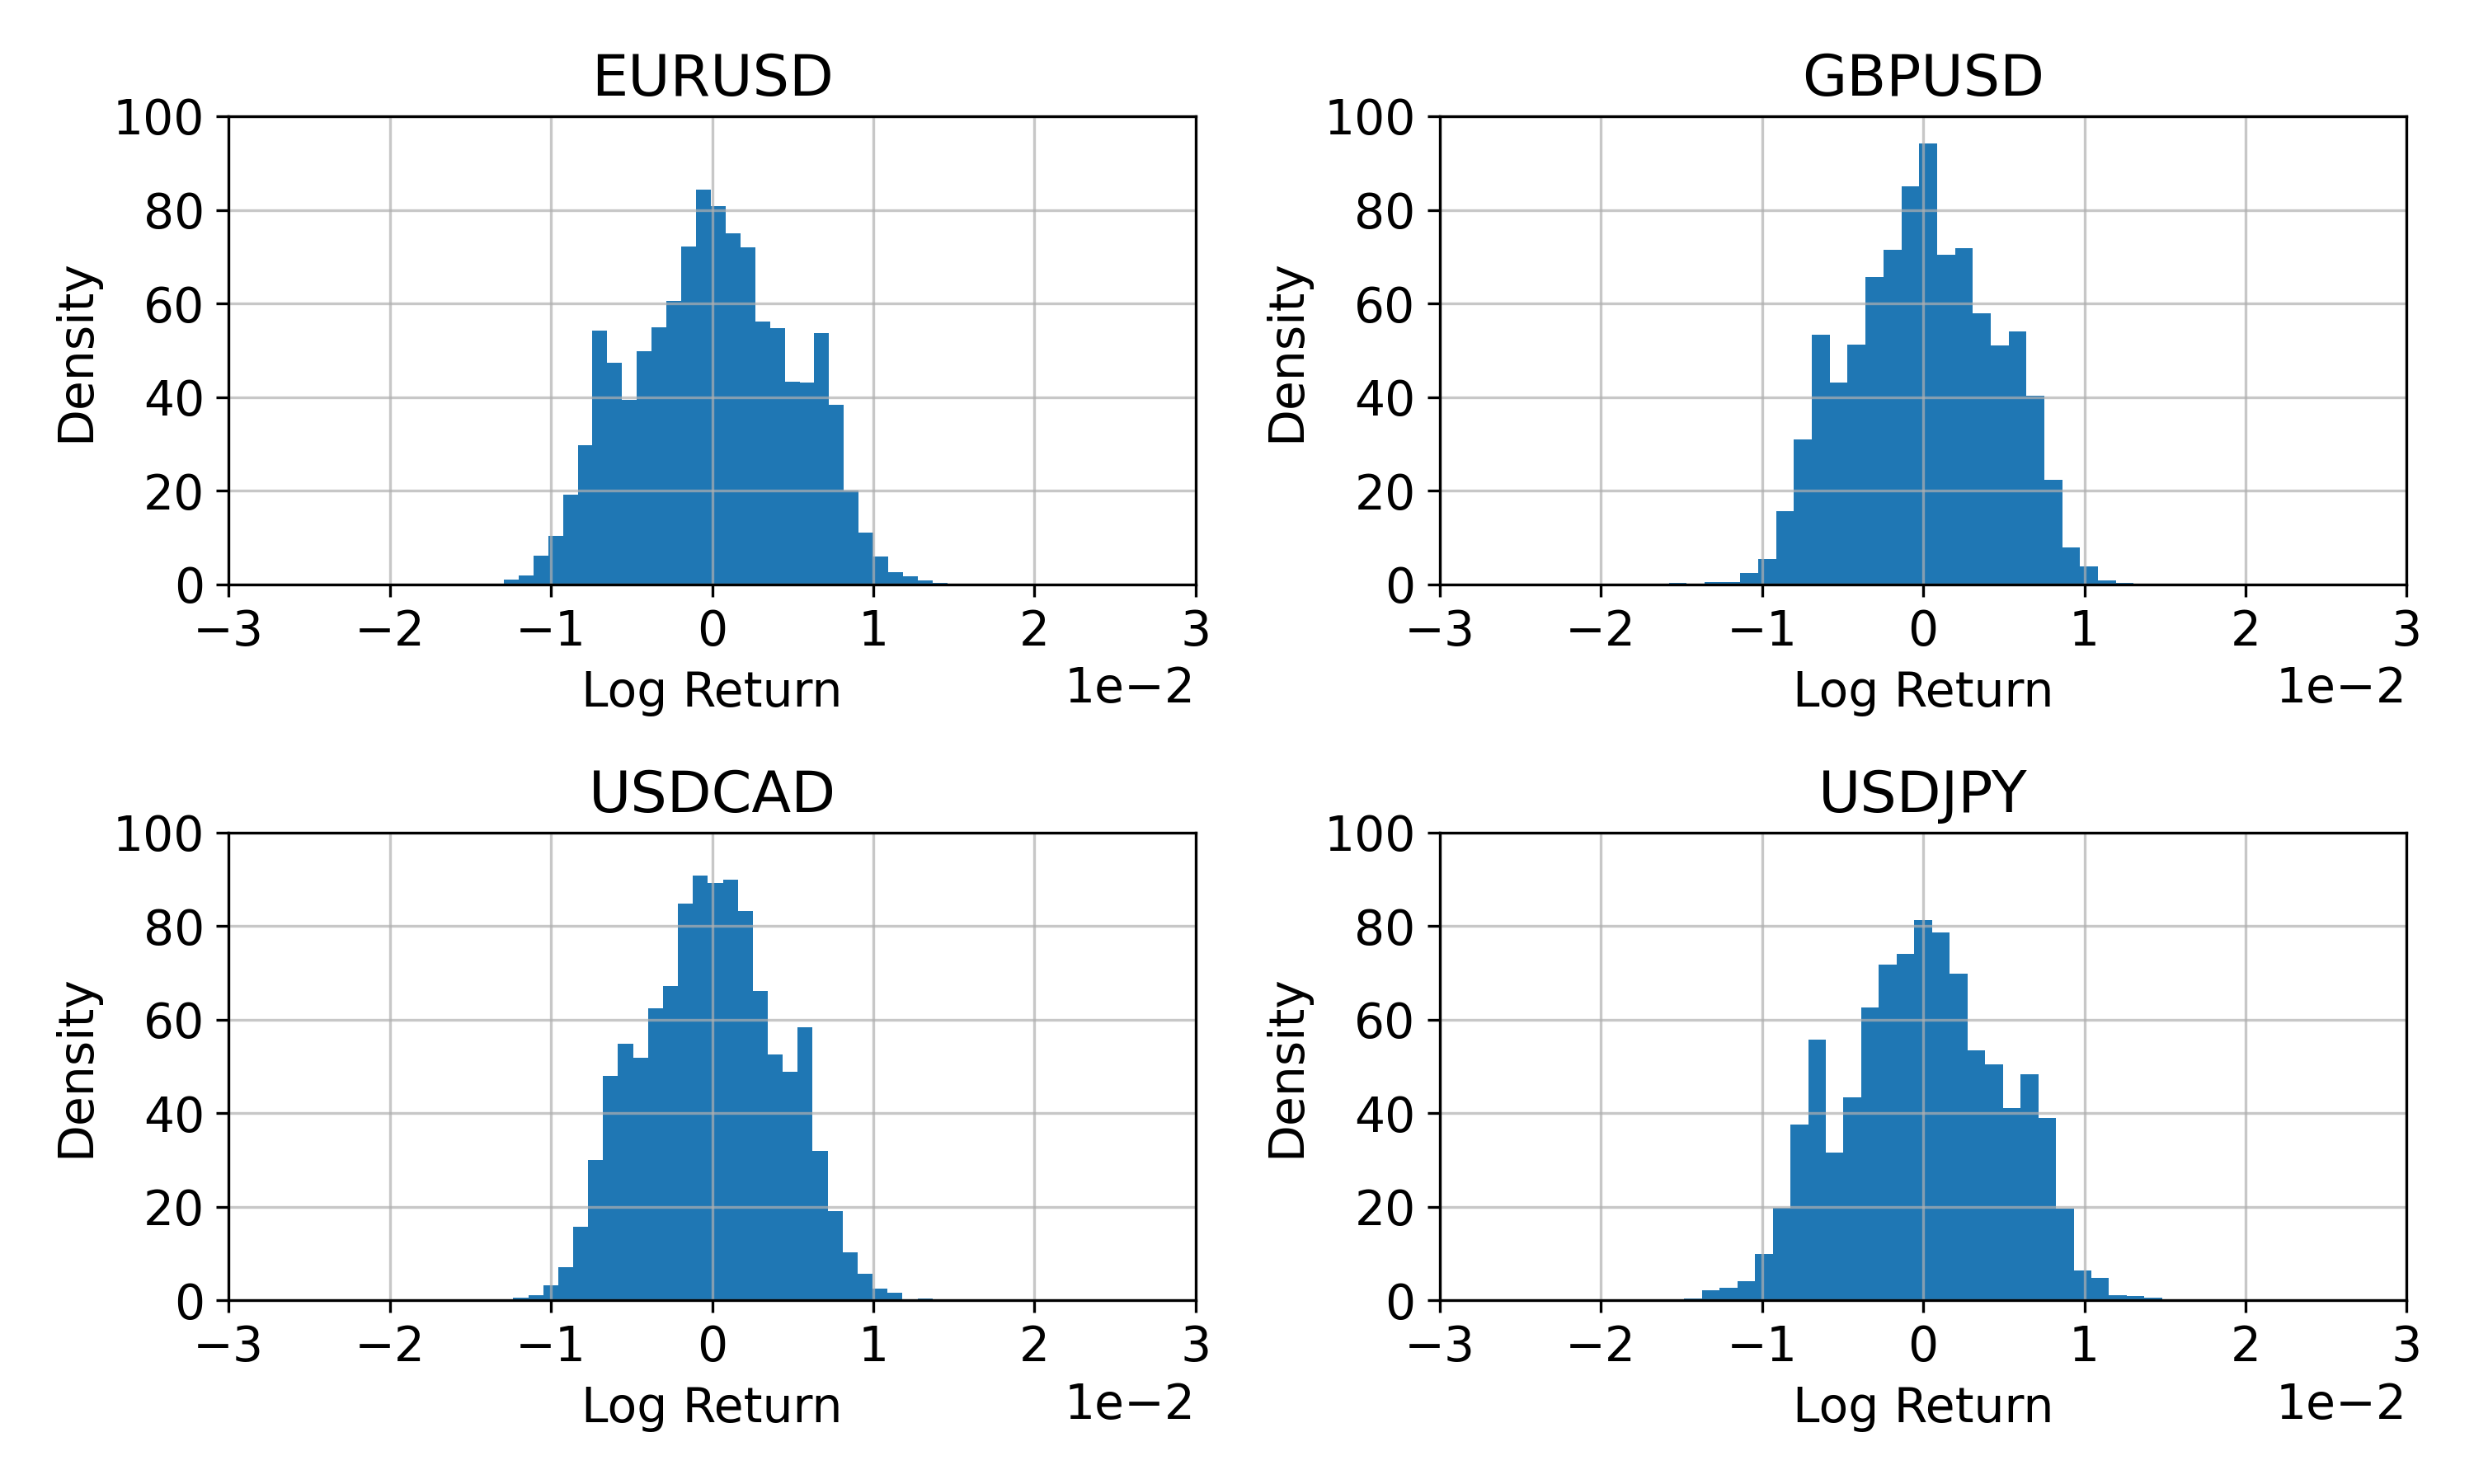
\includegraphics[width=1\linewidth]{data_analysis/histograms_transformed.png}
    \end{figure}
\end{frame}

\begin{frame}
    \frametitle{Transformed Violin/Box Plot}
    \begin{figure}
        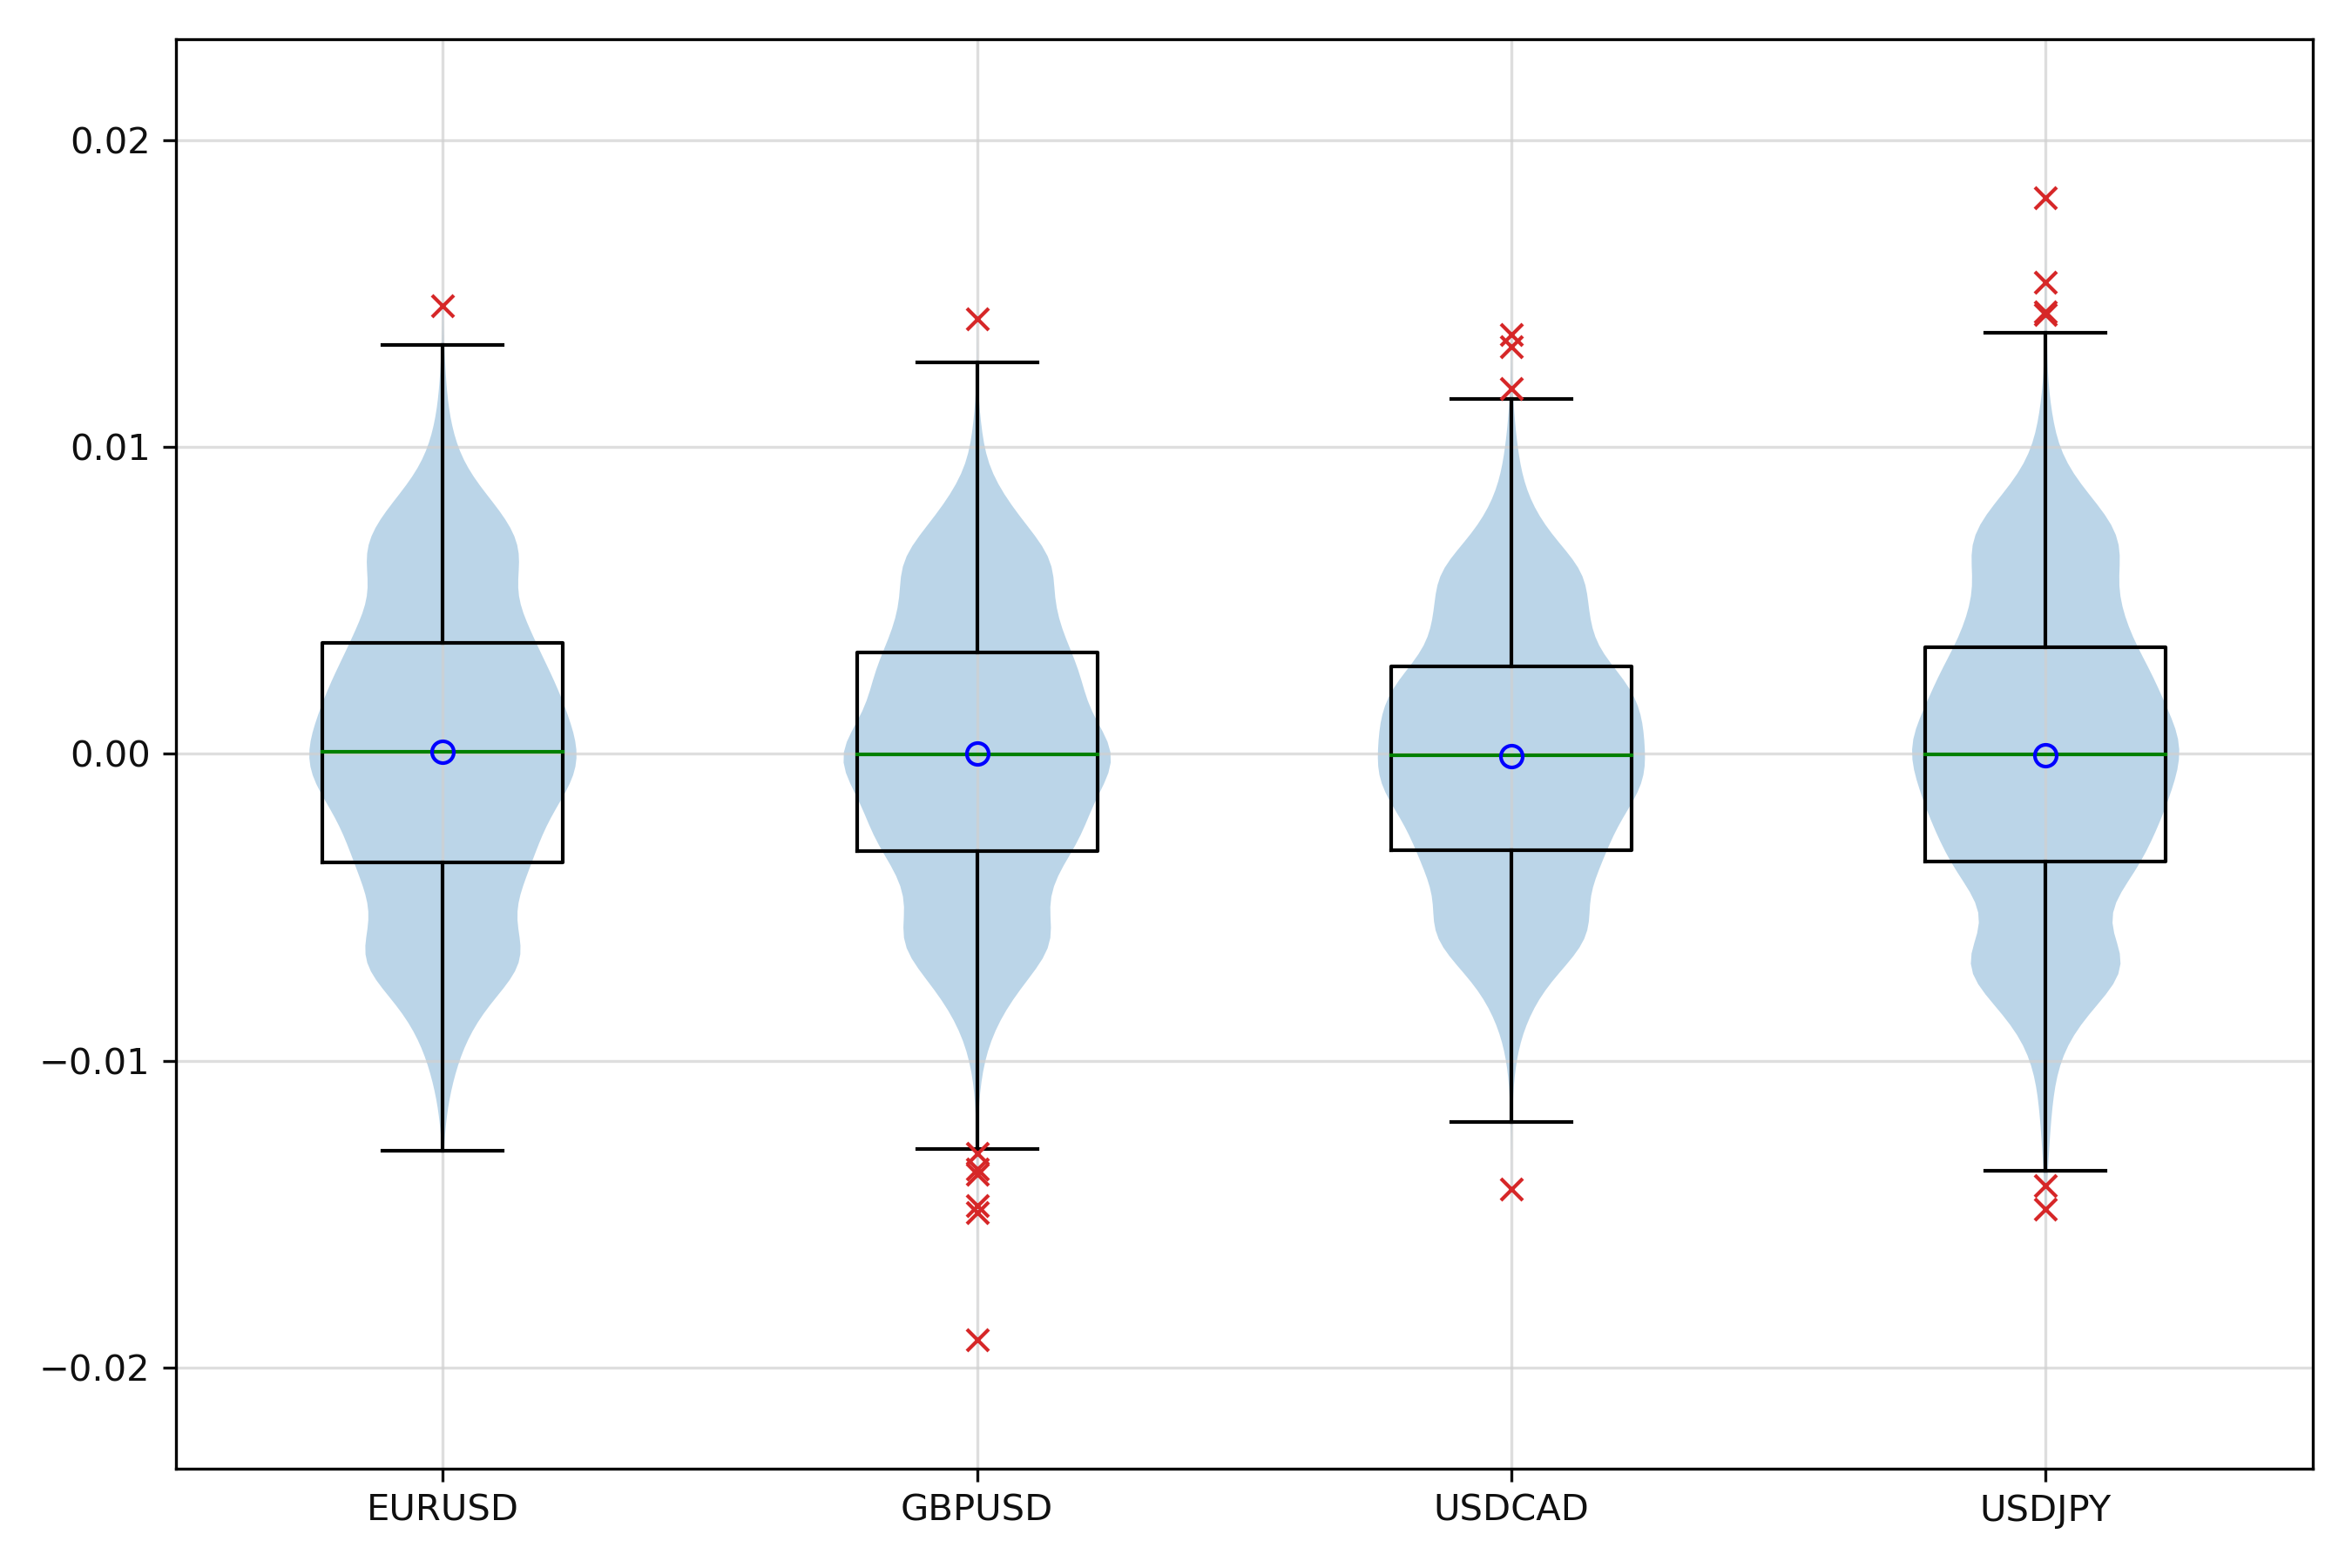
\includegraphics[width=1\linewidth]{data_analysis/violin_transformed.png}
    \end{figure}
\end{frame}

\begin{frame}
    \frametitle{Historical Volatility}
    \begin{figure}
        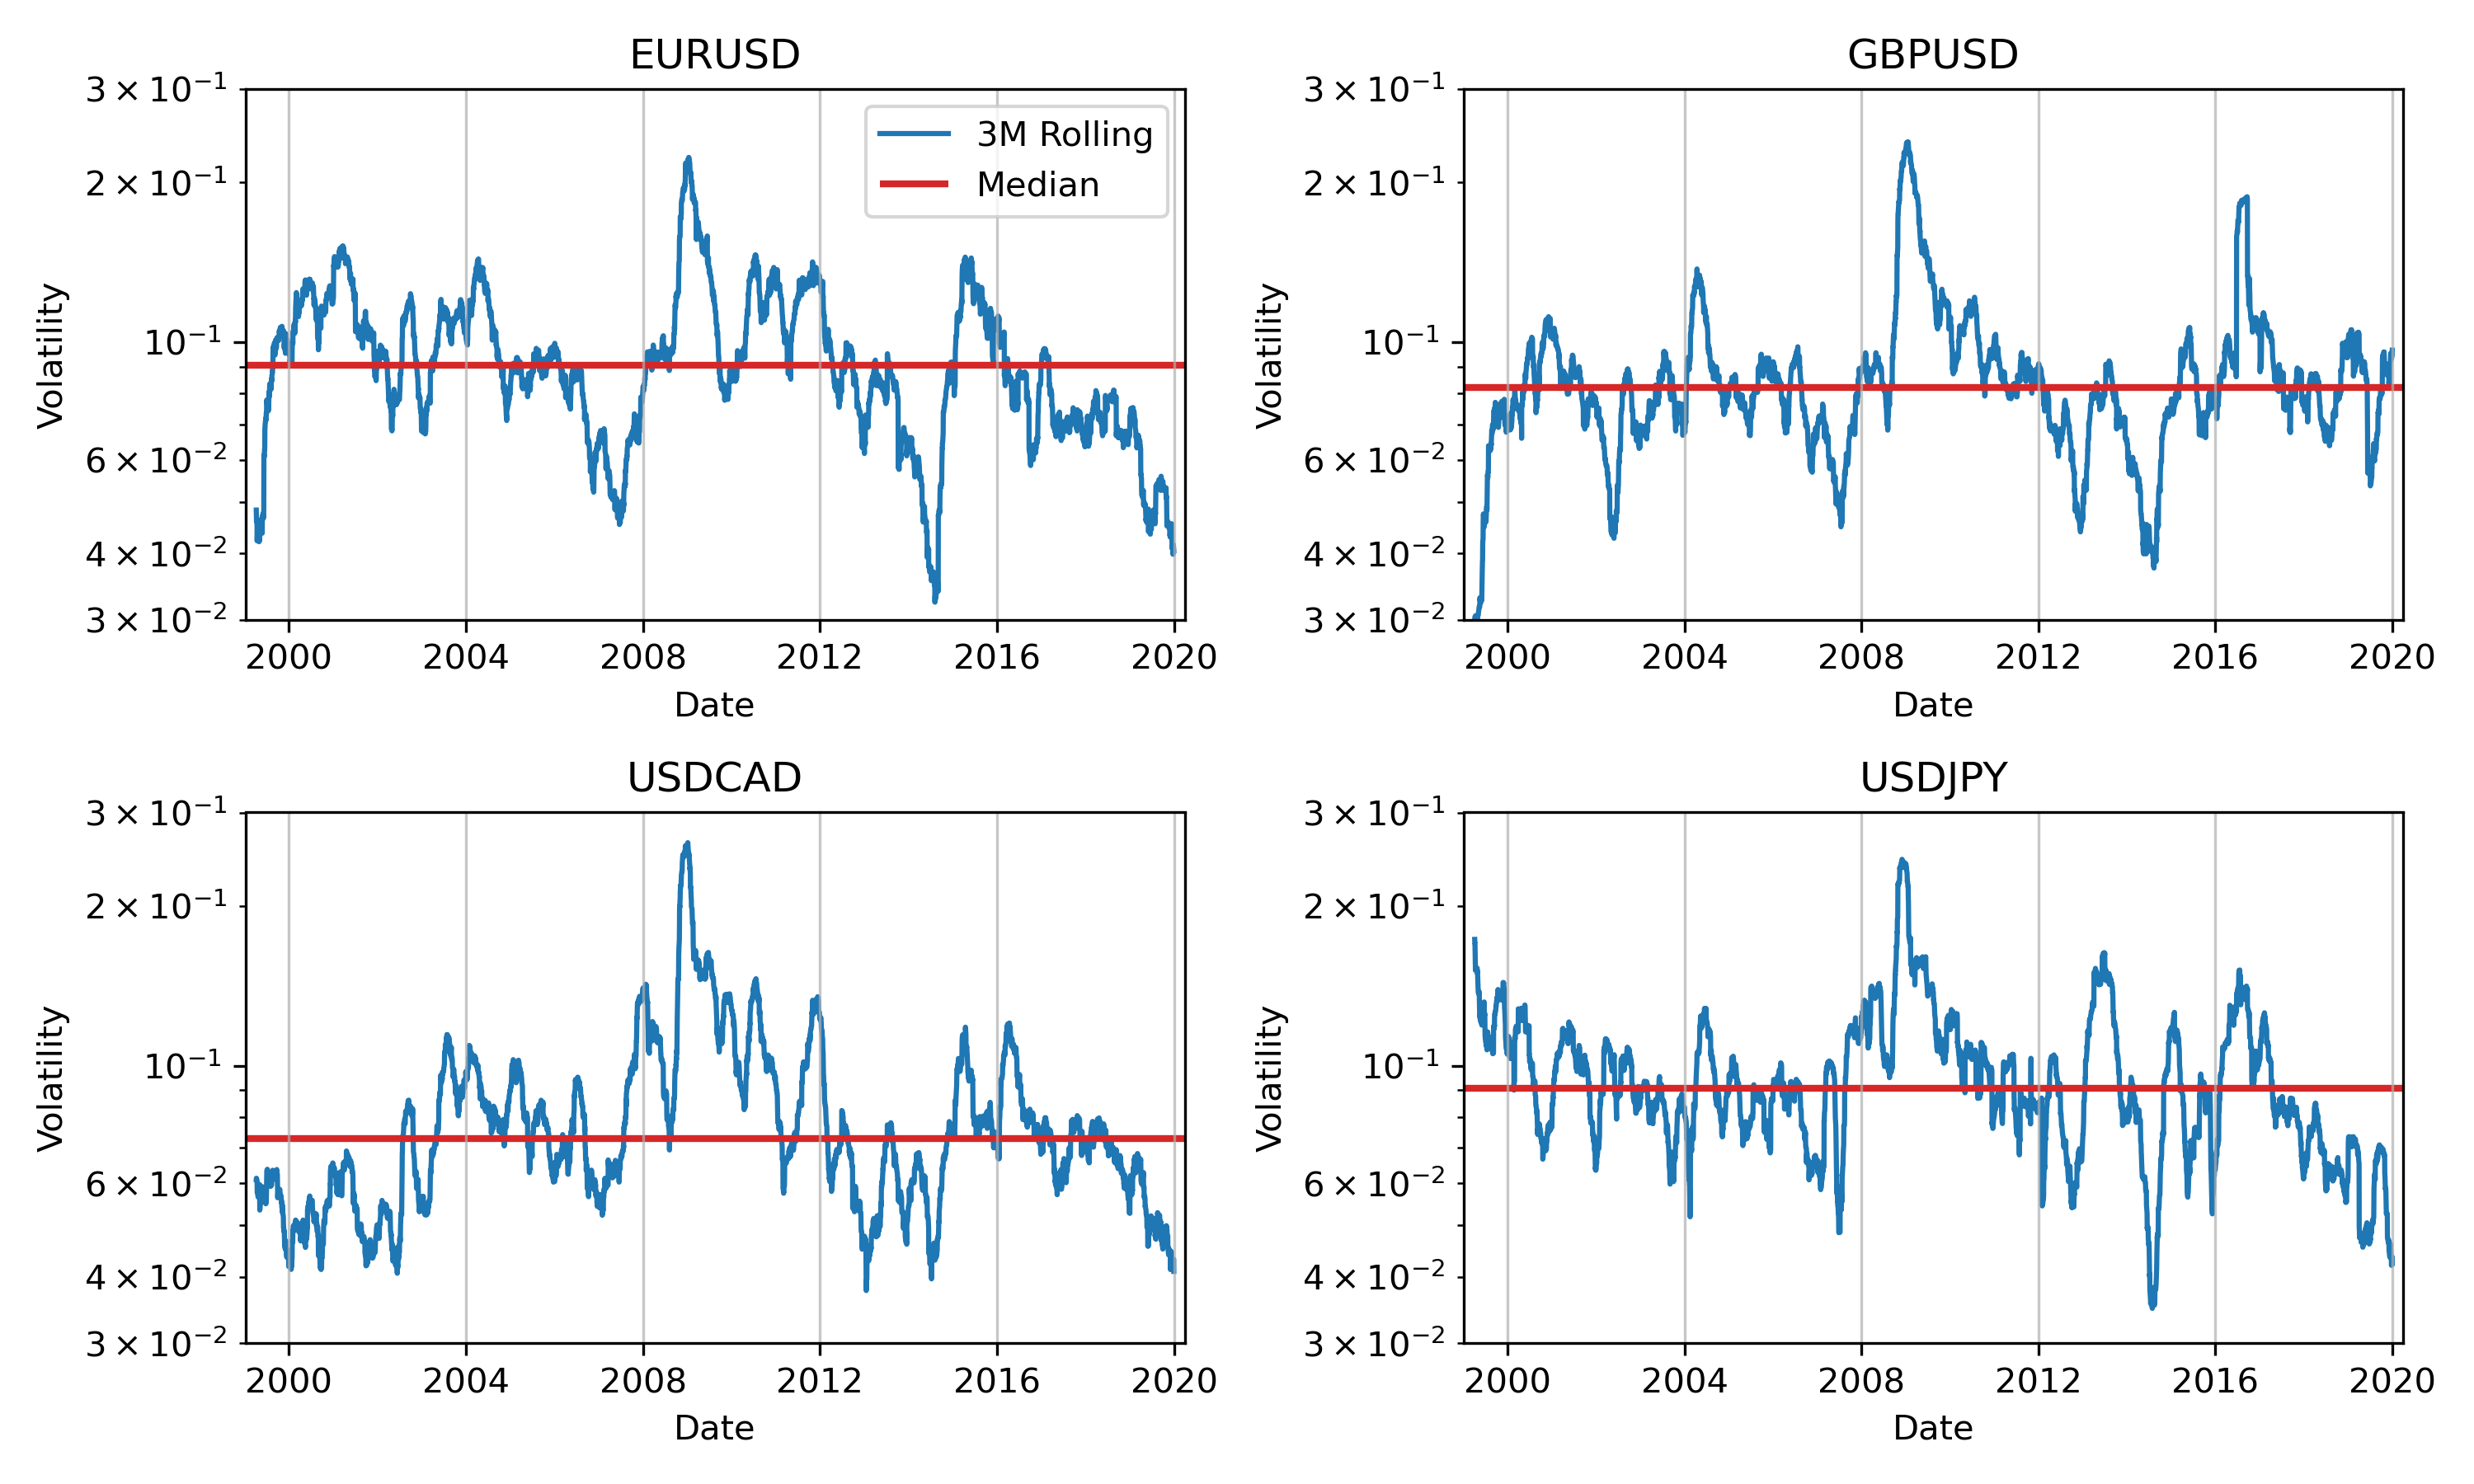
\includegraphics[width=1\linewidth]{data_analysis/rolling_volatility.png}
    \end{figure}
\end{frame}


%----------------------------------------------------------------------------------------
% Classical RBM
%----------------------------------------------------------------------------------------

\section{Classical Restricted Boltzmann Machine (RBM)}

\subsection{Theory}
\begin{frame}
    \frametitle{Classical Restricted Boltzmann Machine (RBM)}
    Model defined by the energy function~\cite{goodfellow_deep_learning}
    \begin{align}
    \begin{split}
        E(\vec{v}, \vec{h})
            &= -\sum_i a_i v_i - \sum_j b_j h_j - \sum_{i,j} v_i w_{ij} h_j
    \end{split}
    \end{align}
    Joint probability distribution (with intractable~\cite{long_servedio_2010} partition function)
    \begin{align}
        p(\vec{v}, \vec{h}) = \frac{1}{Z} e^{-E(\vec{v},\vec{h})}
    \end{align}
    Conditional probabilities
    \begin{align}
    \begin{split}
        p(\vec{h} | \vec{v})
            &= \prod_j \sigma\big( (2\vec{h} - 1) \odot (\vec{b} + \mat{W}^\intercal\vec{v}) \big)_j \\
        p(\vec{v} | \vec{h})
            &= \prod_i \sigma\big( (2\vec{v} - 1) \odot (\vec{a} + \mat{W}\vec{h}) \big)_i
    \end{split}
    \end{align}
\end{frame}

\begin{frame}
    \frametitle{RBM Diagram}
    \begin{figure}
        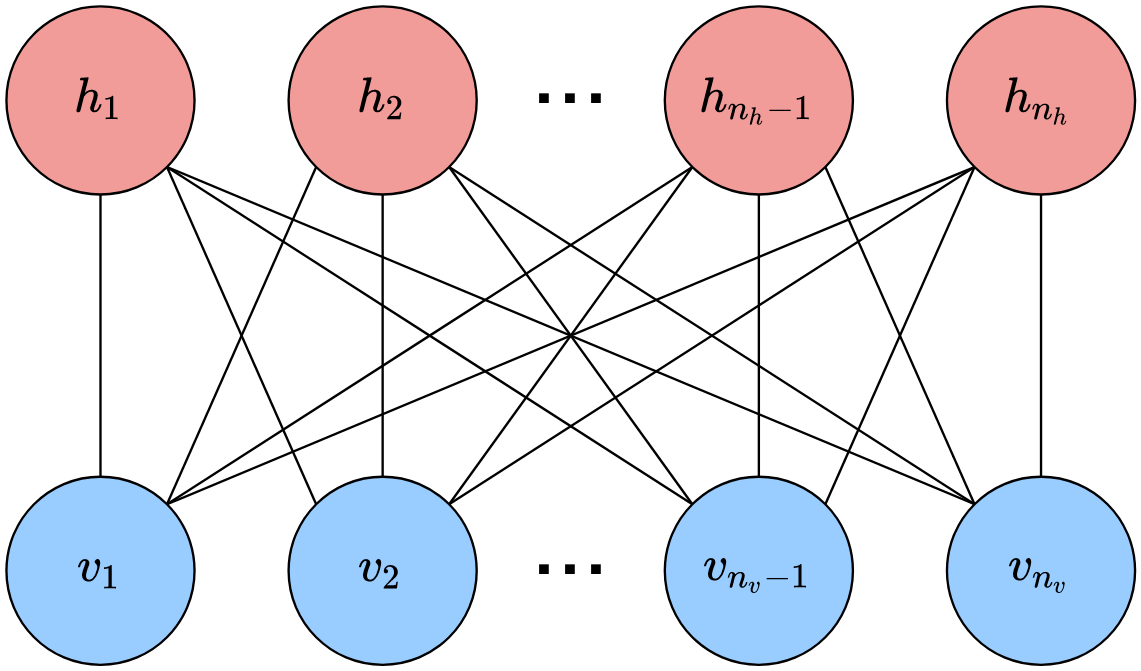
\includegraphics[width=1\linewidth]{rbm_diagram.png}
    \end{figure}
\end{frame}

\begin{frame}
    \frametitle{Log-Likelihood Maximization}
    Log-likelihood
    \begin{align}
    \begin{split}
        \ell(\theta)
            &= \sum_{\vec{v}} p_{\text{data}}(\vec{v}) \log p(\vec{v})
    \end{split}
    \end{align}
    with partial derivatives
    \begin{align}
    \begin{split}
        \partial_{w_{ij}} \ell(\theta)
            &= \langle v_i h_j \rangle_{\text{data}} - \langle v_i h_j \rangle_{\text{model}} \\
        \partial_{a_i} \ell(\theta)
            &= \langle v_i \rangle_{\text{data}} - \langle v_i \rangle_{\text{model}} \\
        \partial_{b_j} \ell(\theta)
            &= \langle h_j \rangle_{\text{data}} - \langle h_j \rangle_{\text{model}}
    \end{split}
    \end{align}
\end{frame}

\begin{frame}
    \frametitle{Gibbs Sampling and Contrastive Divergence}
    The model is sampled using Gibbs sampling, an MCMC method \( \implies \) autocorrelations and thermalization requirements.
    Model is trained using contrastive divergence, which takes training samples, then uses Gibbs sampling for a number of steps (typically 1~\cite{hinton_rbm_training}) to produce model samples for \( \langle \ \cdot \ \rangle_\text{model} \).
    \begin{figure}
        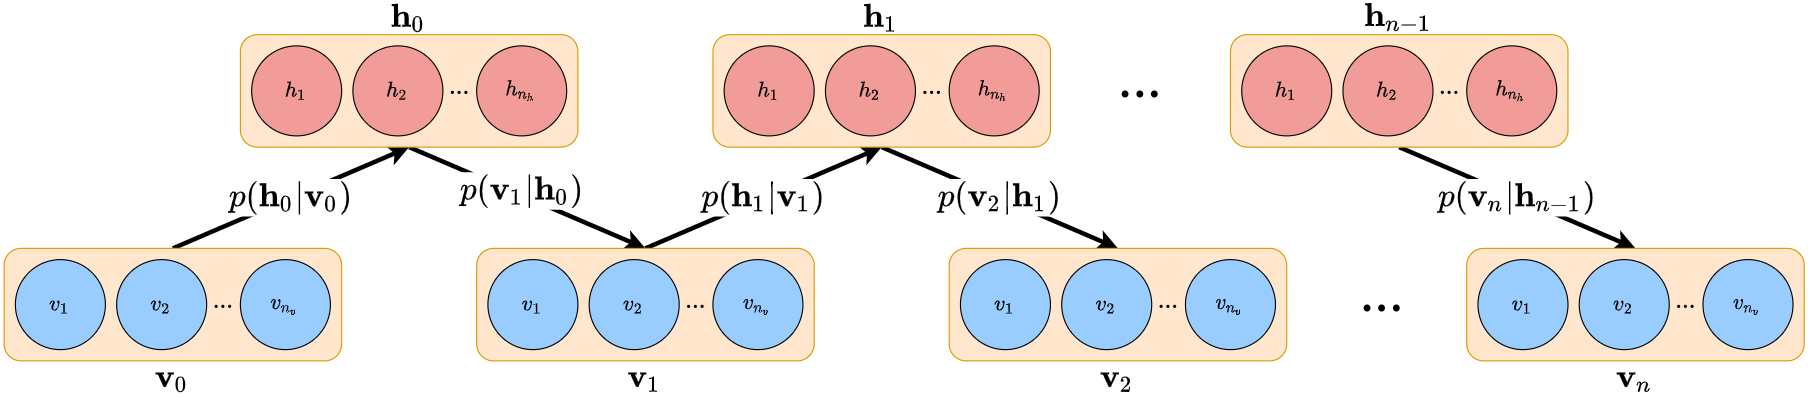
\includegraphics[width=1\linewidth]{gibbs_sampling_diagram.png}
    \end{figure}
\end{frame}

\subsection{The Classical Market Generator}
\begin{frame}
    \frametitle{The Classical Market Generator}
    Idea originated from the paper \textit{The Market Generator}~\cite{kondratyev_2019}.

    We trained and analyzed four different RBM models, each with slightly different preprocessing procedures denoted by:
    \begin{itemize}
        \item (B): trained on the base data set.
        \item (X): trained on the base data set transformed with the outlier power transformation.
        \item (V): trained on the base data set with additional volatility indicators.
        \item (XV): trained on the base data set transformed with the outlier power transformation.
    \end{itemize}
    All values computed from an ensemble of 100 sample sets with \( 10^4 \) samples each.
\end{frame}

\begin{frame}
    \frametitle{Autocorrelation Functions}
    \begin{figure}
        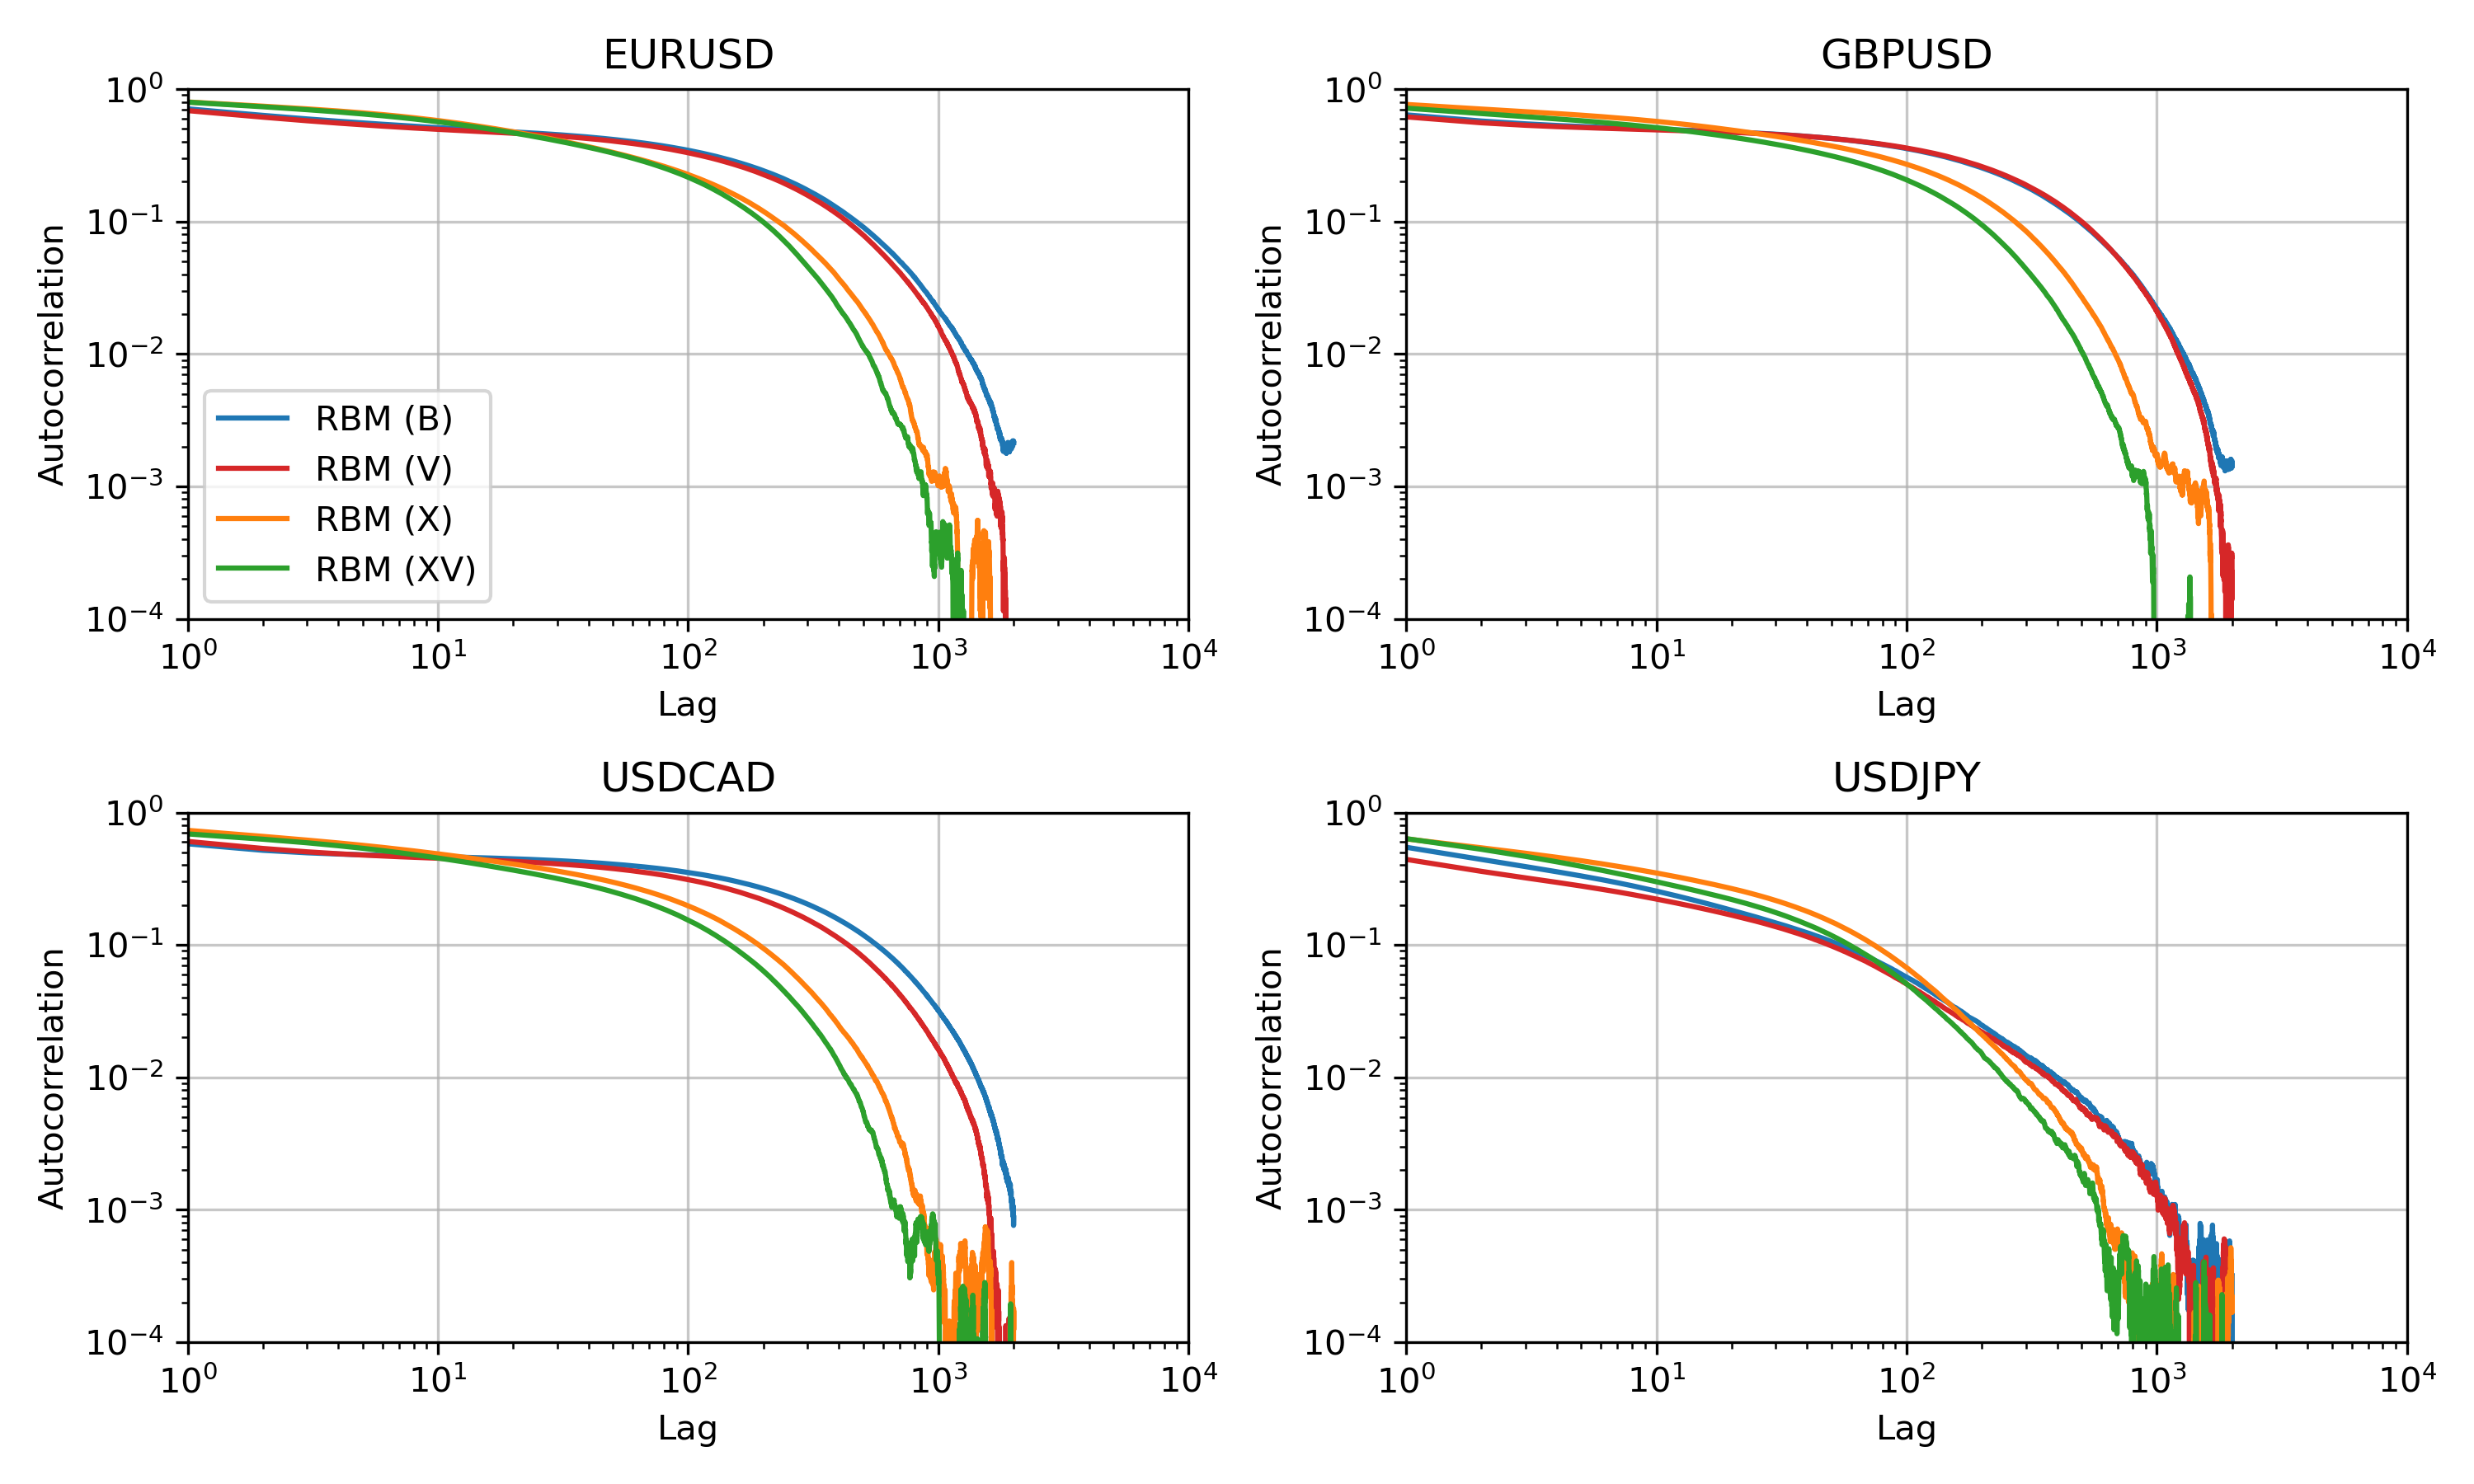
\includegraphics[width=0.9\linewidth]{rbm/autocorrelation_functions.png}
    \end{figure}
\end{frame}

\begin{frame}
    \frametitle{QQ Plots}
    \begin{figure}
        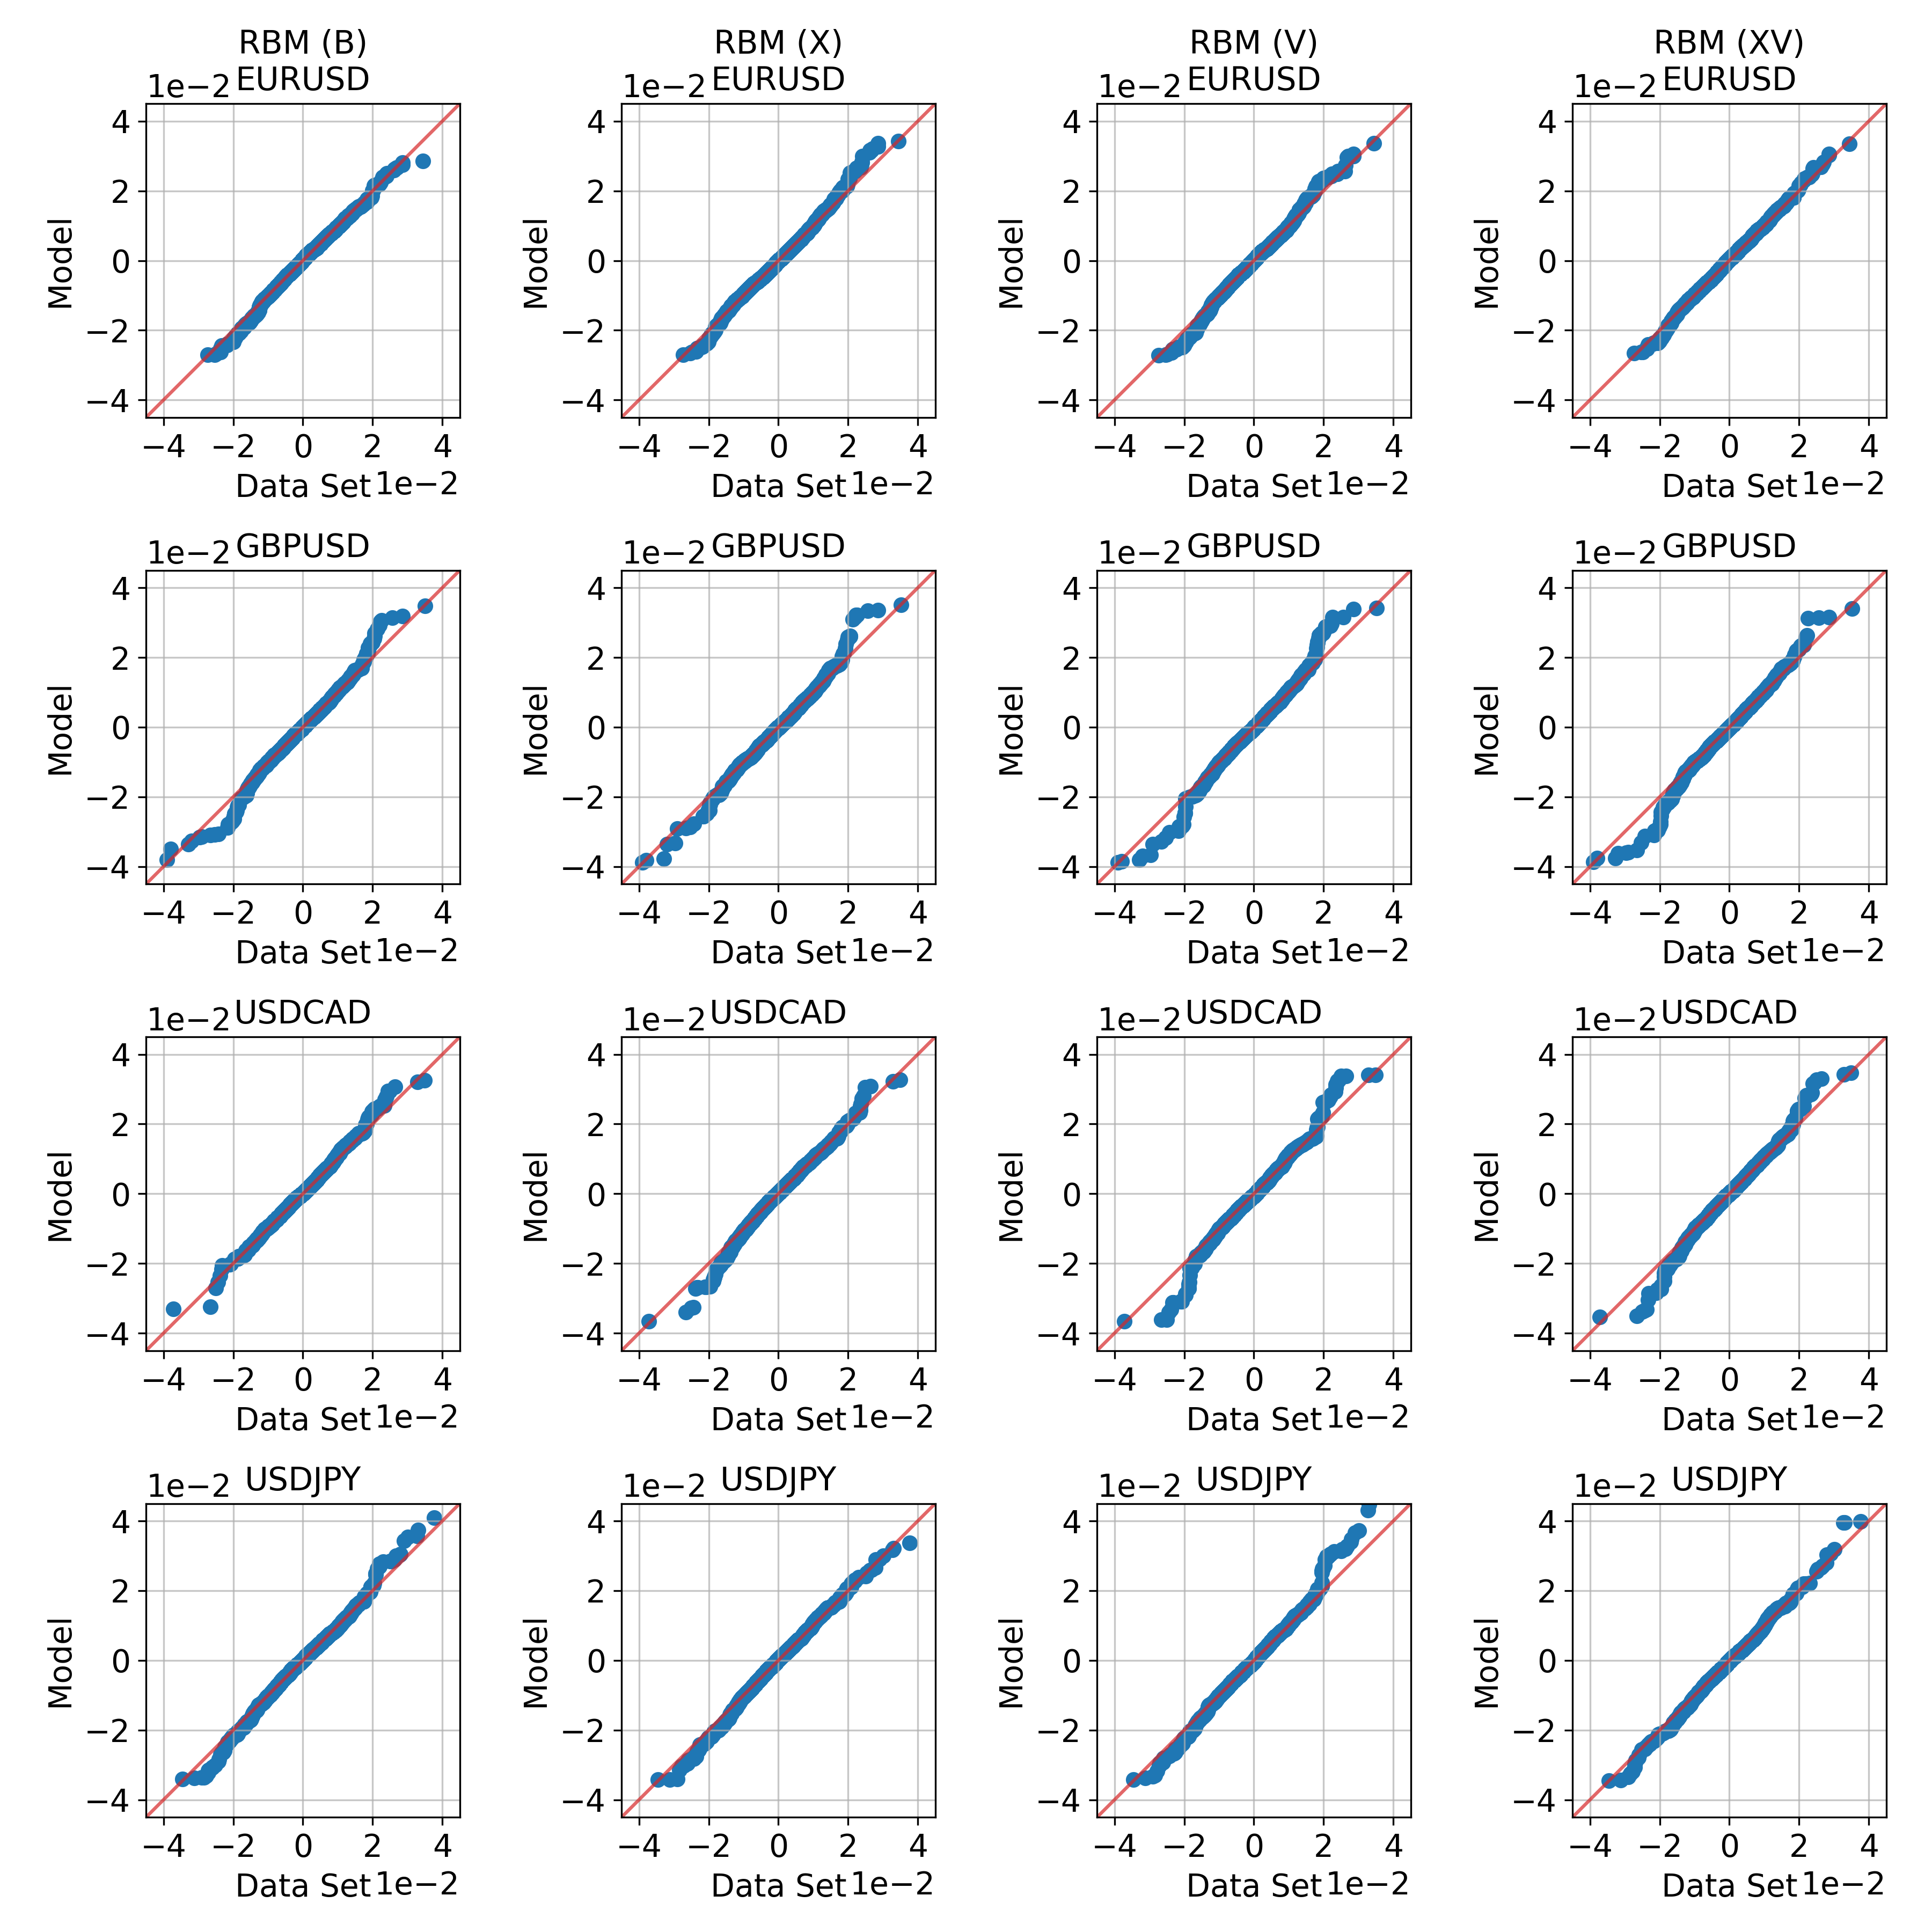
\includegraphics[width=0.65\linewidth]{rbm/qq.png}
    \end{figure}
\end{frame}

\begin{frame}
    \frametitle{KL Divergences}
    \begin{table}[!htb]
        \centering
        \begin{adjustbox}{max width=\textwidth}
            \input{../../tables/rbm/kl_divergences.tbl}
        \end{adjustbox}
    \end{table}
\end{frame}

%\begin{frame}
    %\frametitle{Correlation Coefficients}
    %\begin{table}[!htb]
        %\centering
        %\begin{adjustbox}{max height=35mm}
            %\input{../../tables/rbm/correlation_coefficients.tbl}
        %\end{adjustbox}
    %\end{table}
%\end{frame}

\begin{frame}
    \frametitle{Correlation Coefficients}
    \begin{figure}
        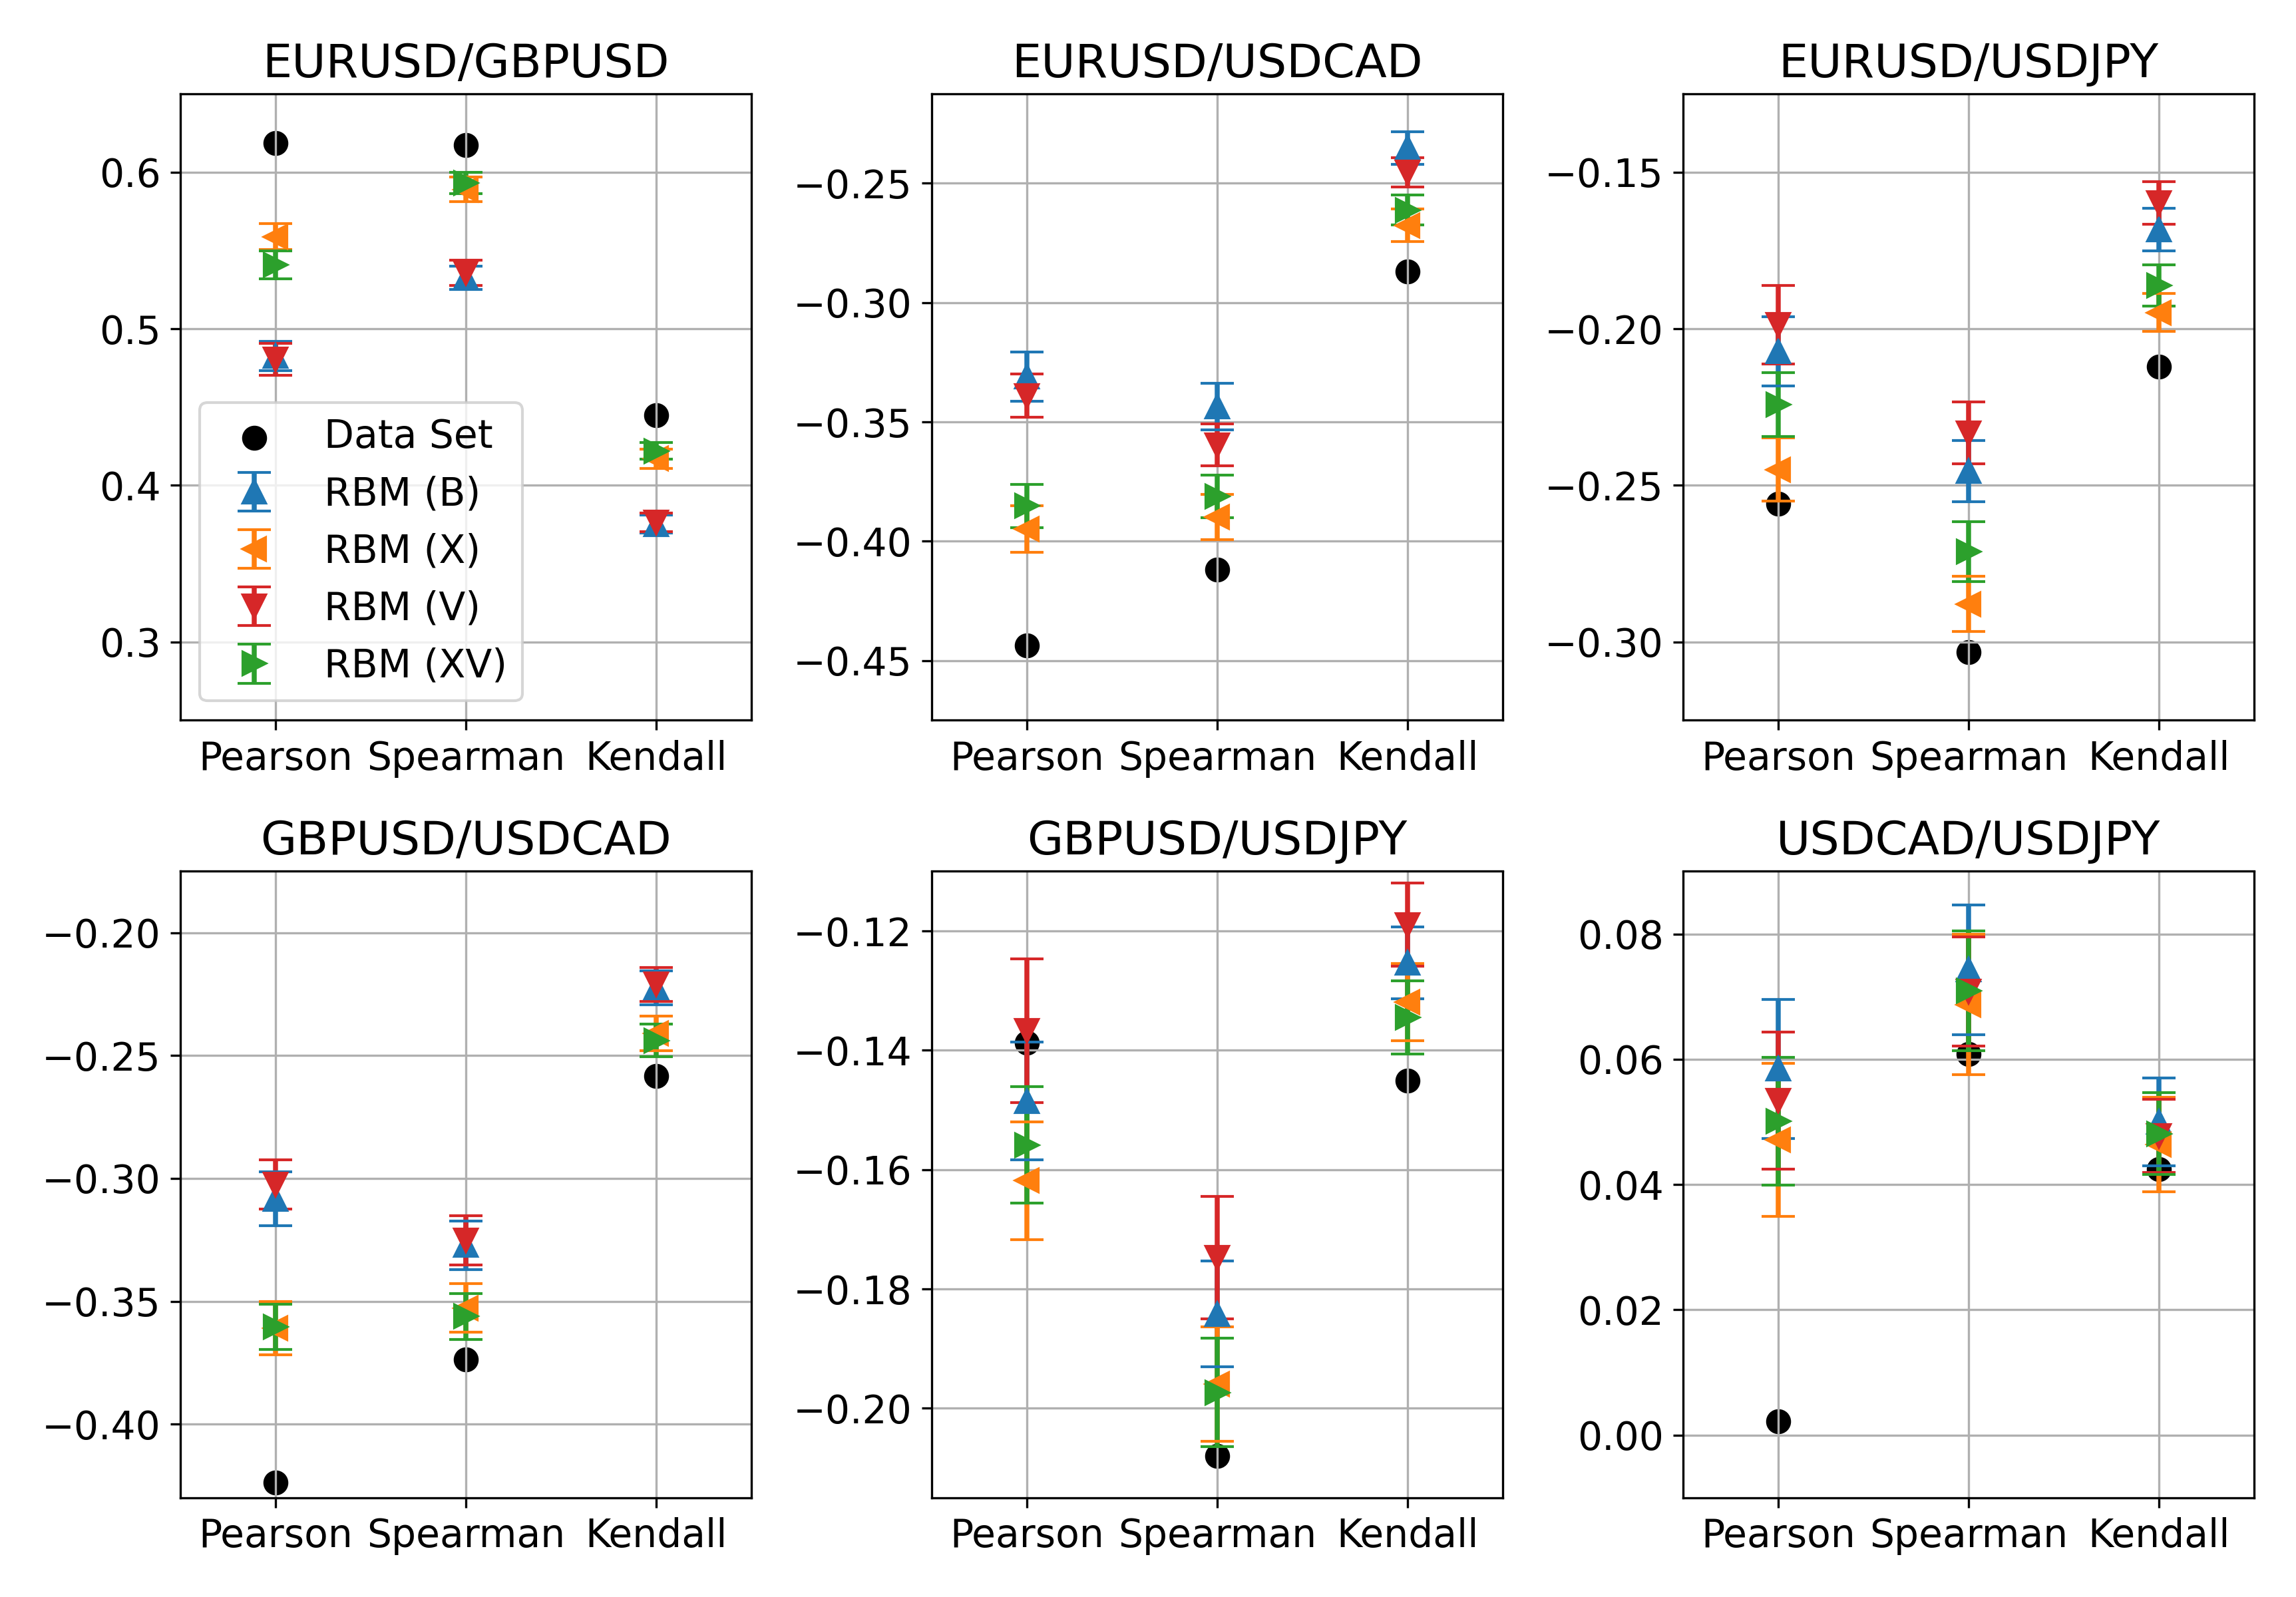
\includegraphics[width=0.9\linewidth]{rbm/correlation_coefficients.png}
    \end{figure}
\end{frame}

\begin{frame}
    \frametitle{Volatilities}
    \begin{table}[!htb]
        \centering
        \begin{adjustbox}{max width=\textwidth}
            \input{../../tables/rbm/volatilities.tbl}
        \end{adjustbox}
    \end{table}
\end{frame}

\begin{frame}
    \frametitle{Tails}
    \begin{table}[!htb]
        \centering
        \begin{adjustbox}{max width=\textwidth}
            \input{../../tables/rbm/tails.tbl}
        \end{adjustbox}
    \end{table}
\end{frame}

\begin{frame}
    \frametitle{Conditional Sampling}
    \begin{table}[!htb]
        \centering
        \begin{adjustbox}{max width=\textwidth}
            \input{../../tables/rbm/conditional_volatilities.tbl}
        \end{adjustbox}
    \end{table}
\end{frame}

%----------------------------------------------------------------------------------------
% Quantum Boltzmann Machines
%----------------------------------------------------------------------------------------

\section{Quantum Boltzmann Machine (QBM)}

\subsection{Theory}
\begin{frame}
    \frametitle{Quantum Boltzmann Machine (QBM)}
    Hamiltonian~\cite{amin_2018}
    \begin{align}
        H = -\sum_i \Gamma_i \sigma_i^x -\sum_i b_i \sigma_i^z - \sum_{i,j} w_{ij} \sigma_i^z \sigma_j^z
    \end{align}
    and corresponding density operator
    \begin{align}
        \rho = \frac{1}{Z} e^{-H}
    \end{align}
    where \( Z = \tr(e^{-H}) \) is the partition function.
\end{frame}

\begin{frame}
    \frametitle{QBM Optimization}
    Log-likelihood lower bound
    \begin{align}
        \tilde{\ell}(\theta) = \sum_{\vec{v}} \pdata(\vec{v}) \log \tr(\rho_\vec{v})
    \end{align}
    Clamped Hamiltonian
    \begin{align}
        H_\vec{v}
            &= \braket{\vec{v}|H|\vec{v}}
    \end{align}
    and corresponding density operator
    \begin{align}
        \rho_\vec{v}
            &= \frac{1}{Z_\vec{v}} e^{-H_\vec{v}}
    \end{align}
\end{frame}

\begin{frame}
    \frametitle{QBM Optimization}
    Log-likelihood lower bound partial derivatives
    \begin{align}
    \begin{split}
        \partial_{w_{ij}} \tilde{\ell}(\theta)
            &= \langle \sigma_i^z \sigma_j^z \rangle_\text{data} - \langle \sigma_i^z \sigma_j^z \rangle_\text{model} \\
        \partial_{b_i} \tilde{\ell}(\theta)
            &= \langle \sigma_i^z \rangle_\text{data} - \langle \sigma_i^z \rangle_\text{model}
    \end{split}
    \end{align}
    where
    \begin{align}
    \begin{split}
        \langle \sigma_i^z \rangle_\text{data}
            &= \sum_\vec{v} \pdata(\vec{v}) v_i,
            \ i \in \mathcal{I}_v \\
        \langle \sigma_i^z \sigma_j^z \rangle_\text{data}
            &= \sum_\vec{v} \pdata(\vec{v}) v_i v_j,
            \ i, j \in \mathcal{I}_v \\
        \langle \sigma_i^z \rangle_\text{data}
            &= \sum_\vec{v} \pdata(\vec{v}) \frac{b_i'(\vec{v})}{D_i(\vec{v})} \tanh\big(D_i(\vec{v})\big),
            \ i \in \mathcal{I}_h \\
        \langle \sigma_i^z \sigma_j^z \rangle_\text{data}
            &= \sum_\vec{v} \pdata(\vec{v}) v_i \frac{b_j'(\vec{v})}{D_j(\vec{v})} \tanh\big(D_j(\vec{v})\big),
            \ i \in \mathcal{I}_v, \ j \in \mathcal{I}_h
    \end{split}
    \end{align}
\end{frame}

\begin{frame}
    \frametitle{Connection to D-Wave Quantum Annealers}
    D-Wave Hamiltonian~\cite{dwave_qa}
    \begin{align}
        H(s) = A(s) \bigg( -\sum_i \sigma_i^x \bigg) + B(s) \bigg( \sum_i h_i \sigma_i^z + \sum_{i,j} J_{ij} \sigma_i^z \sigma_j^z \bigg)
    \end{align}
    with density operator (\( \beta = 1 / k_B T \))
    \begin{align}
        \rho(s, T) = \frac{1}{Z} e^{-\beta H(s)}
    \end{align}
    Comparing the two yields
    \begin{align}
    \begin{split}
        \Gamma_i
            &= \beta A(s^*) \\
        b_i
            &= -\beta B(s^*) h_i \\
        w_{ij}
            &= -\beta B(s^*) J_{ij}
        \label{eq:qbm_scaling}
    \end{split}
    \end{align}
\end{frame}

\begin{frame}
    \frametitle{Pause-and-Quench Anneal Schedule}
    \begin{figure}
        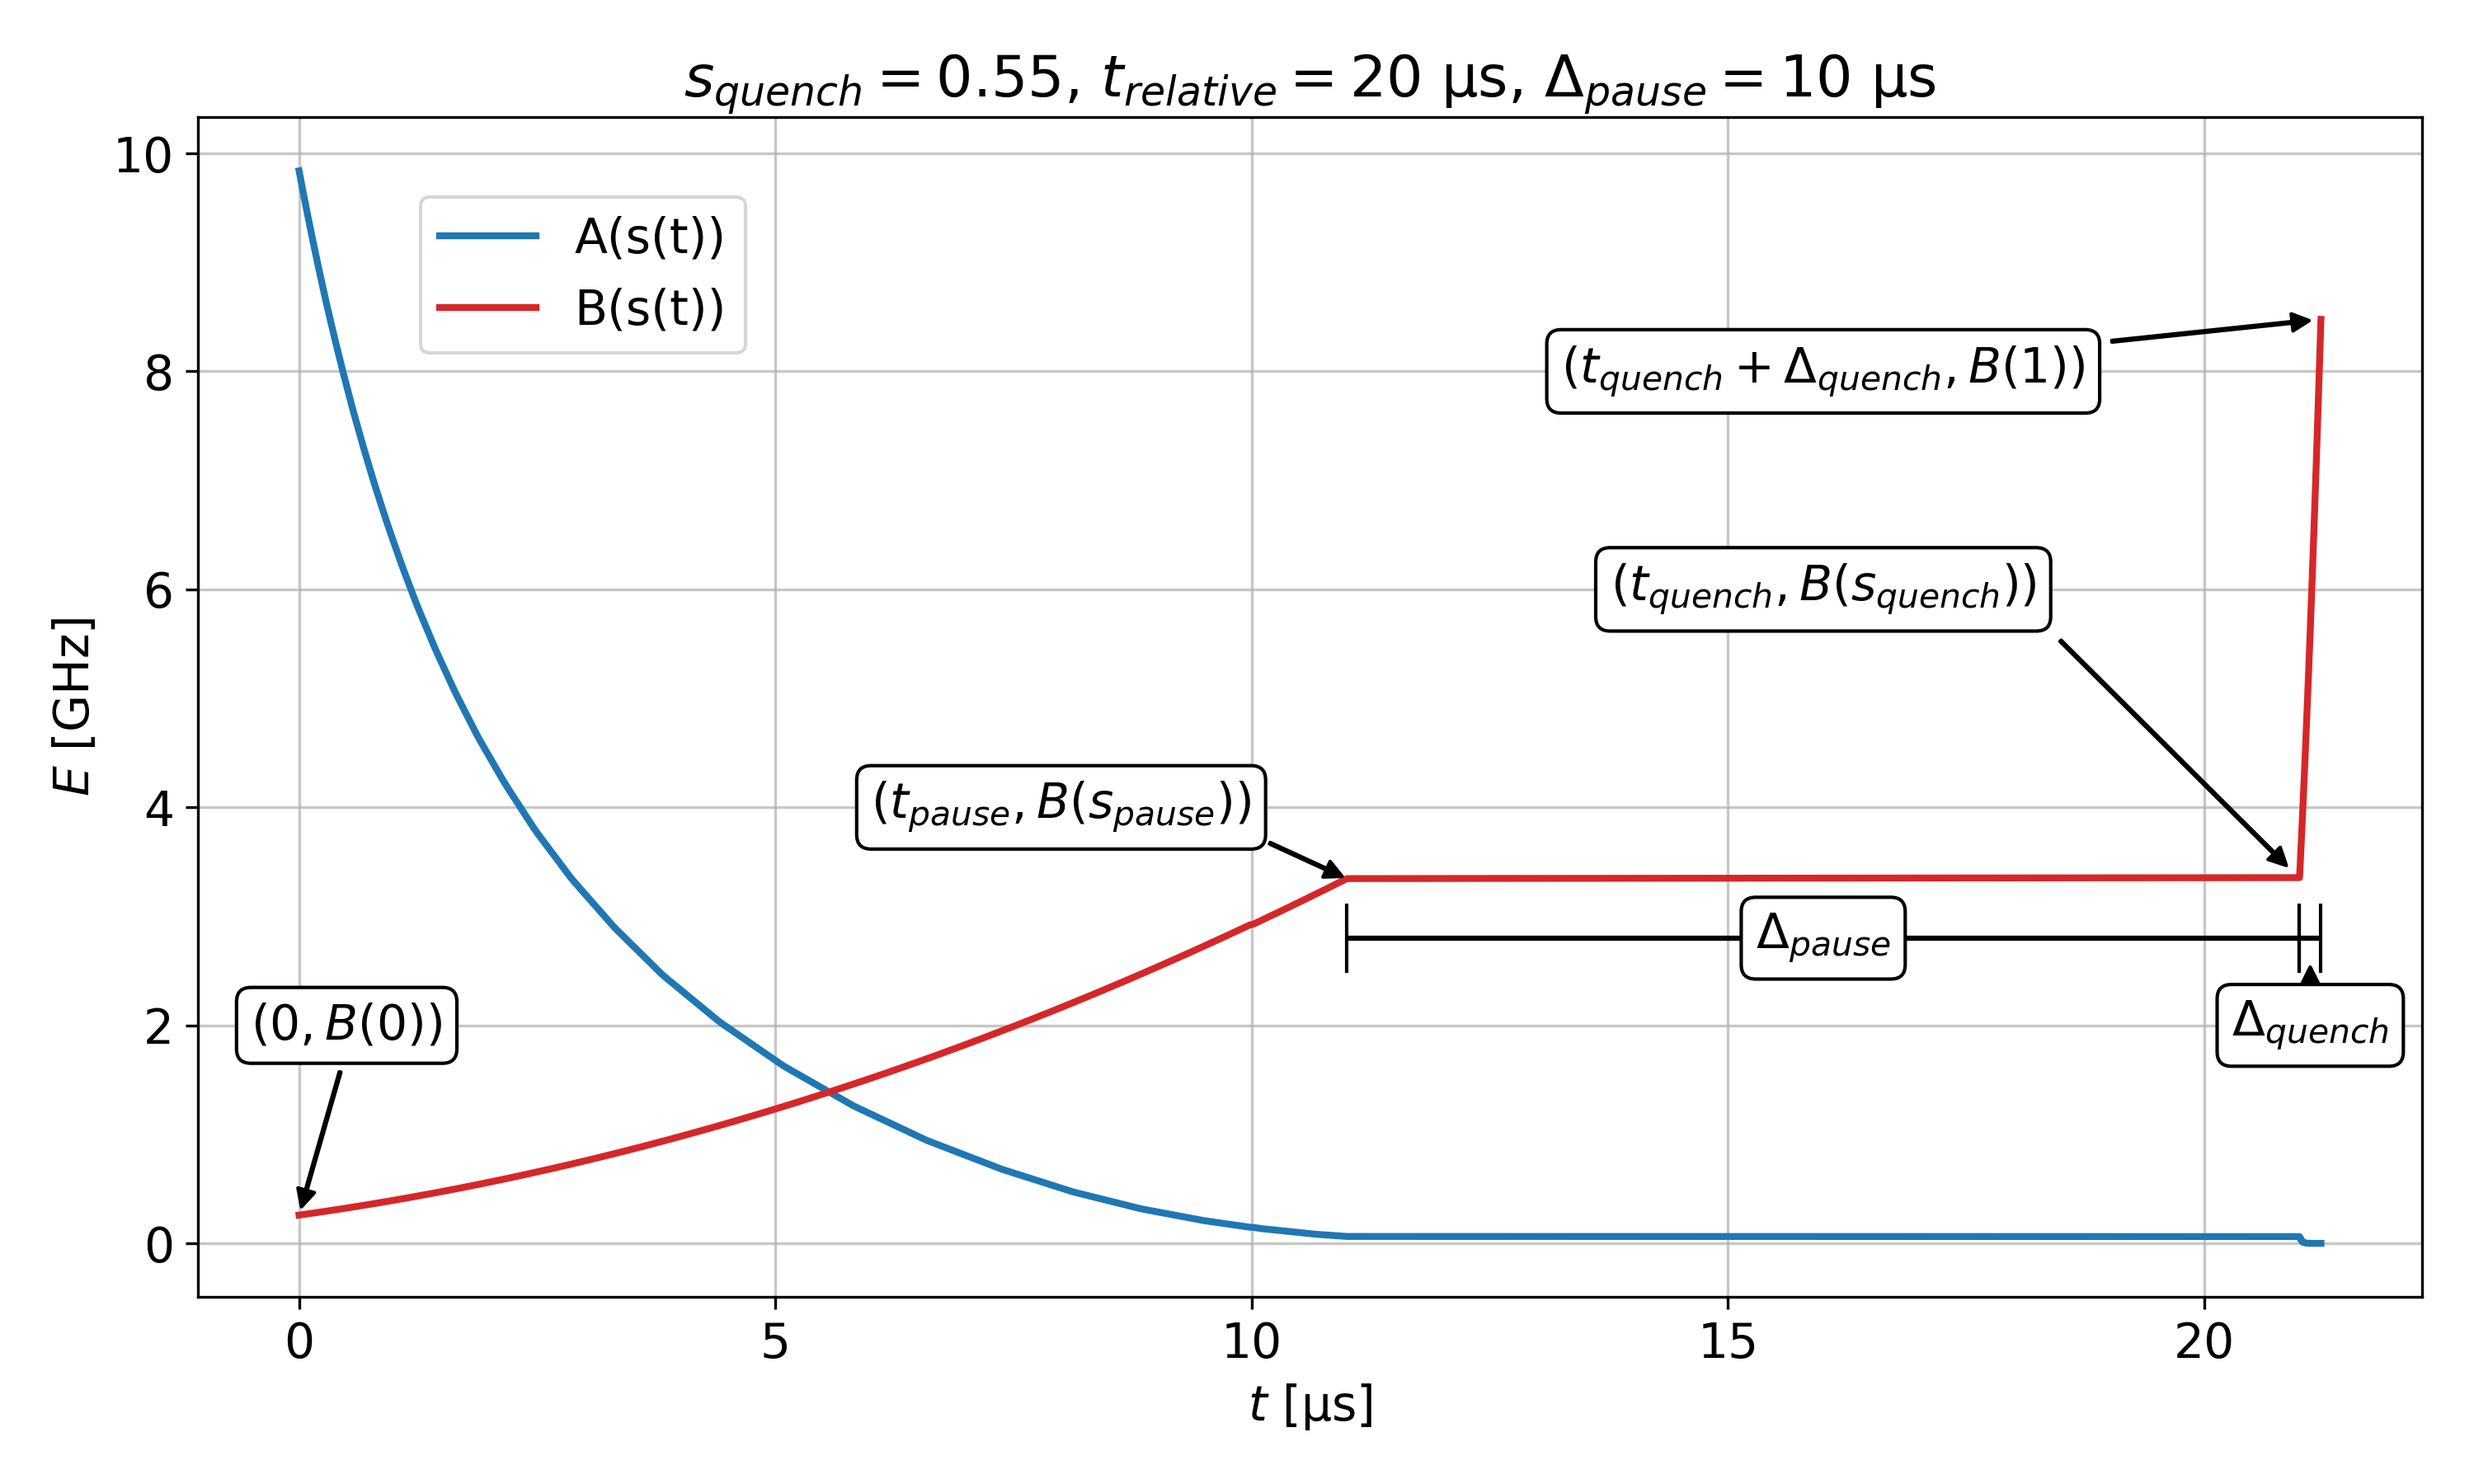
\includegraphics[width=1\linewidth]{qbm/anneal_schedules/Advantage_system4.1-s_pause=0.55-pause_duration=10.png}
    \end{figure}
\end{frame}

\subsection{12-Qubit Problem}
\begin{frame}
    \frametitle{Matching Samples to Theory}
    Values for this analysis represent an ensemble average over 10 random gauges with \( 10^4 \) samples each.
    \begin{figure}
        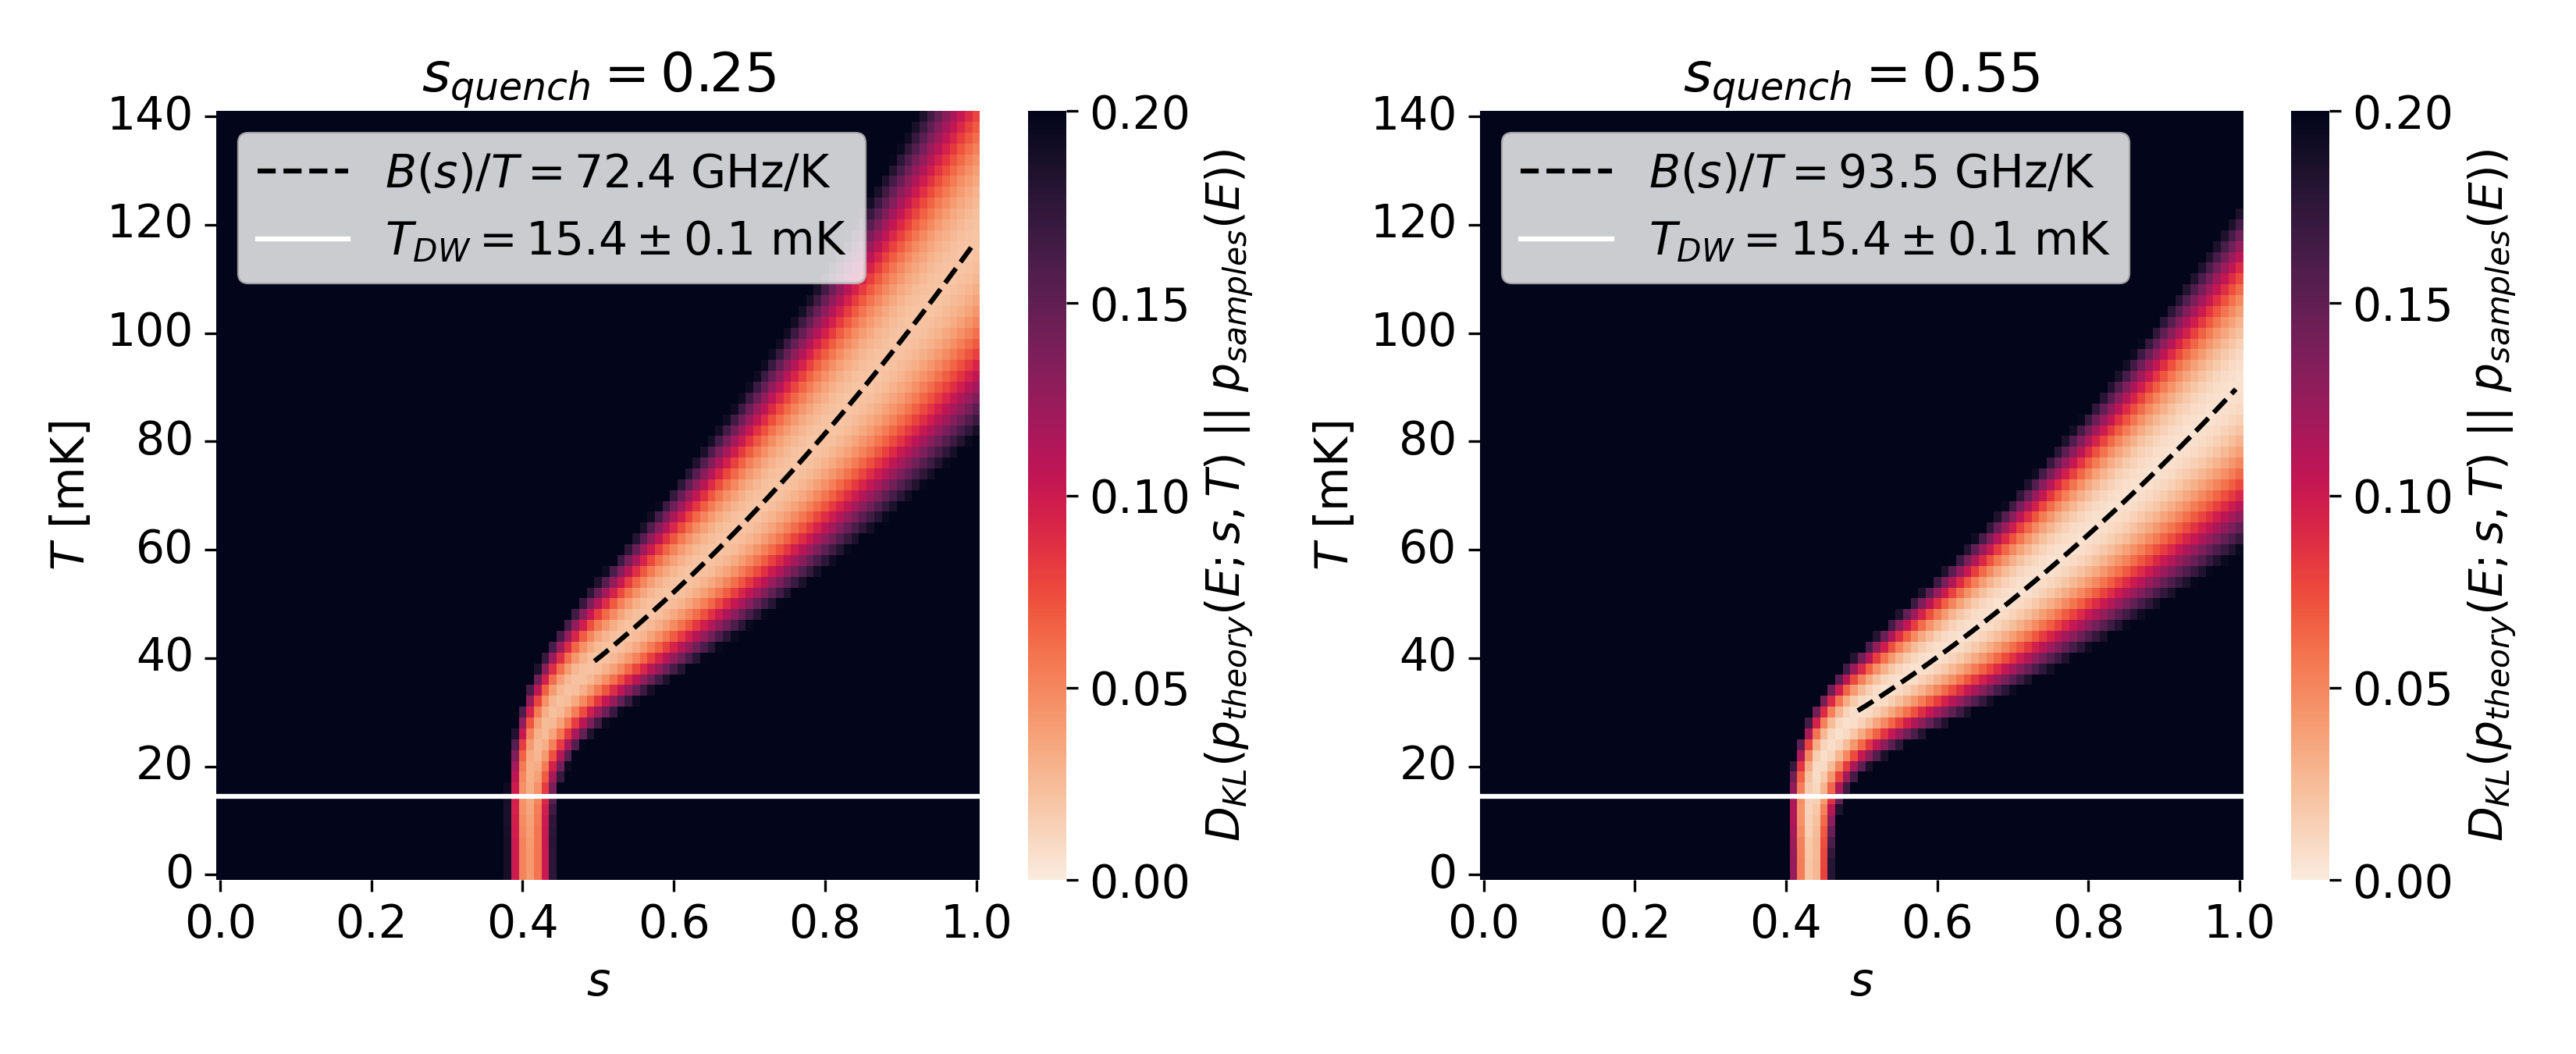
\includegraphics[width=1\linewidth]{qbm/8x4/embedding_comparison/config_05/dkl_min_heatmap-embedding=10.png}
    \end{figure}
\end{frame}

\begin{frame}
    \frametitle{Embedding Comparison}
    All embeddings were direct, i.e., no chains were used.
    \begin{figure}
        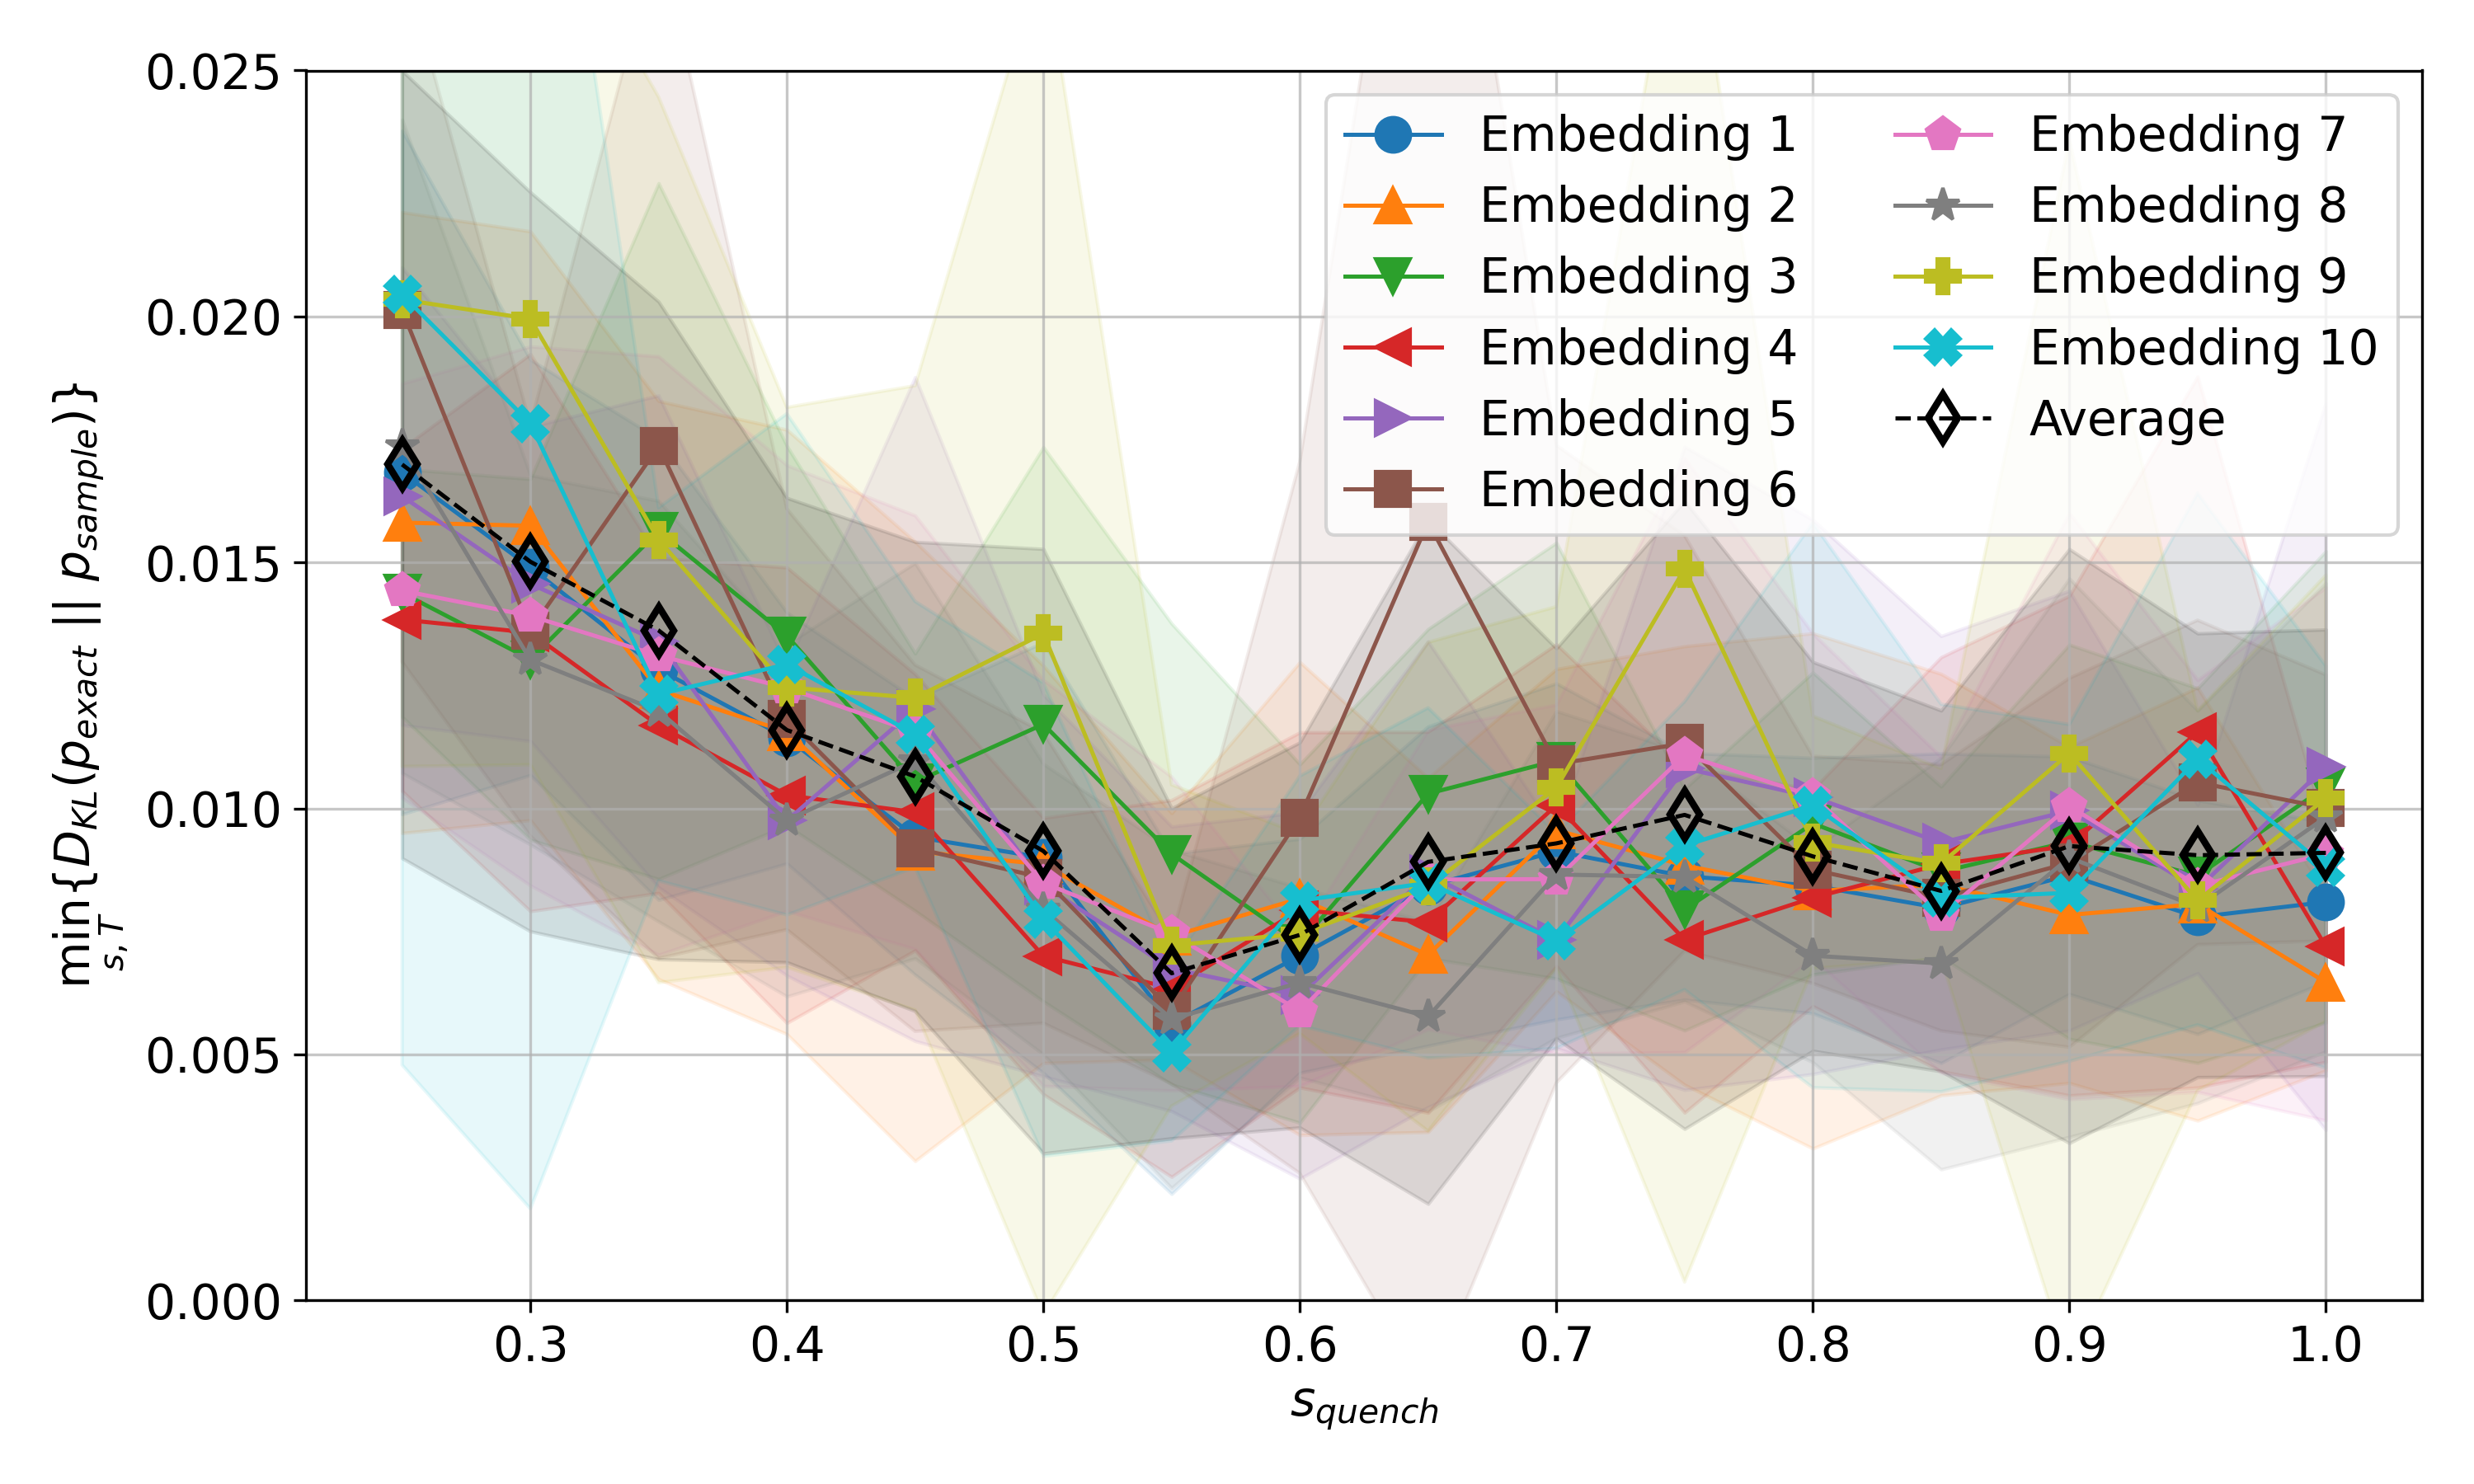
\includegraphics[width=1\linewidth]{qbm/8x4/embedding_comparison/config_05/kl_divergence_mins.png}
    \end{figure}
\end{frame}

\begin{frame}
    \frametitle{Anneal Schedule Comparison}
    \begin{figure}
        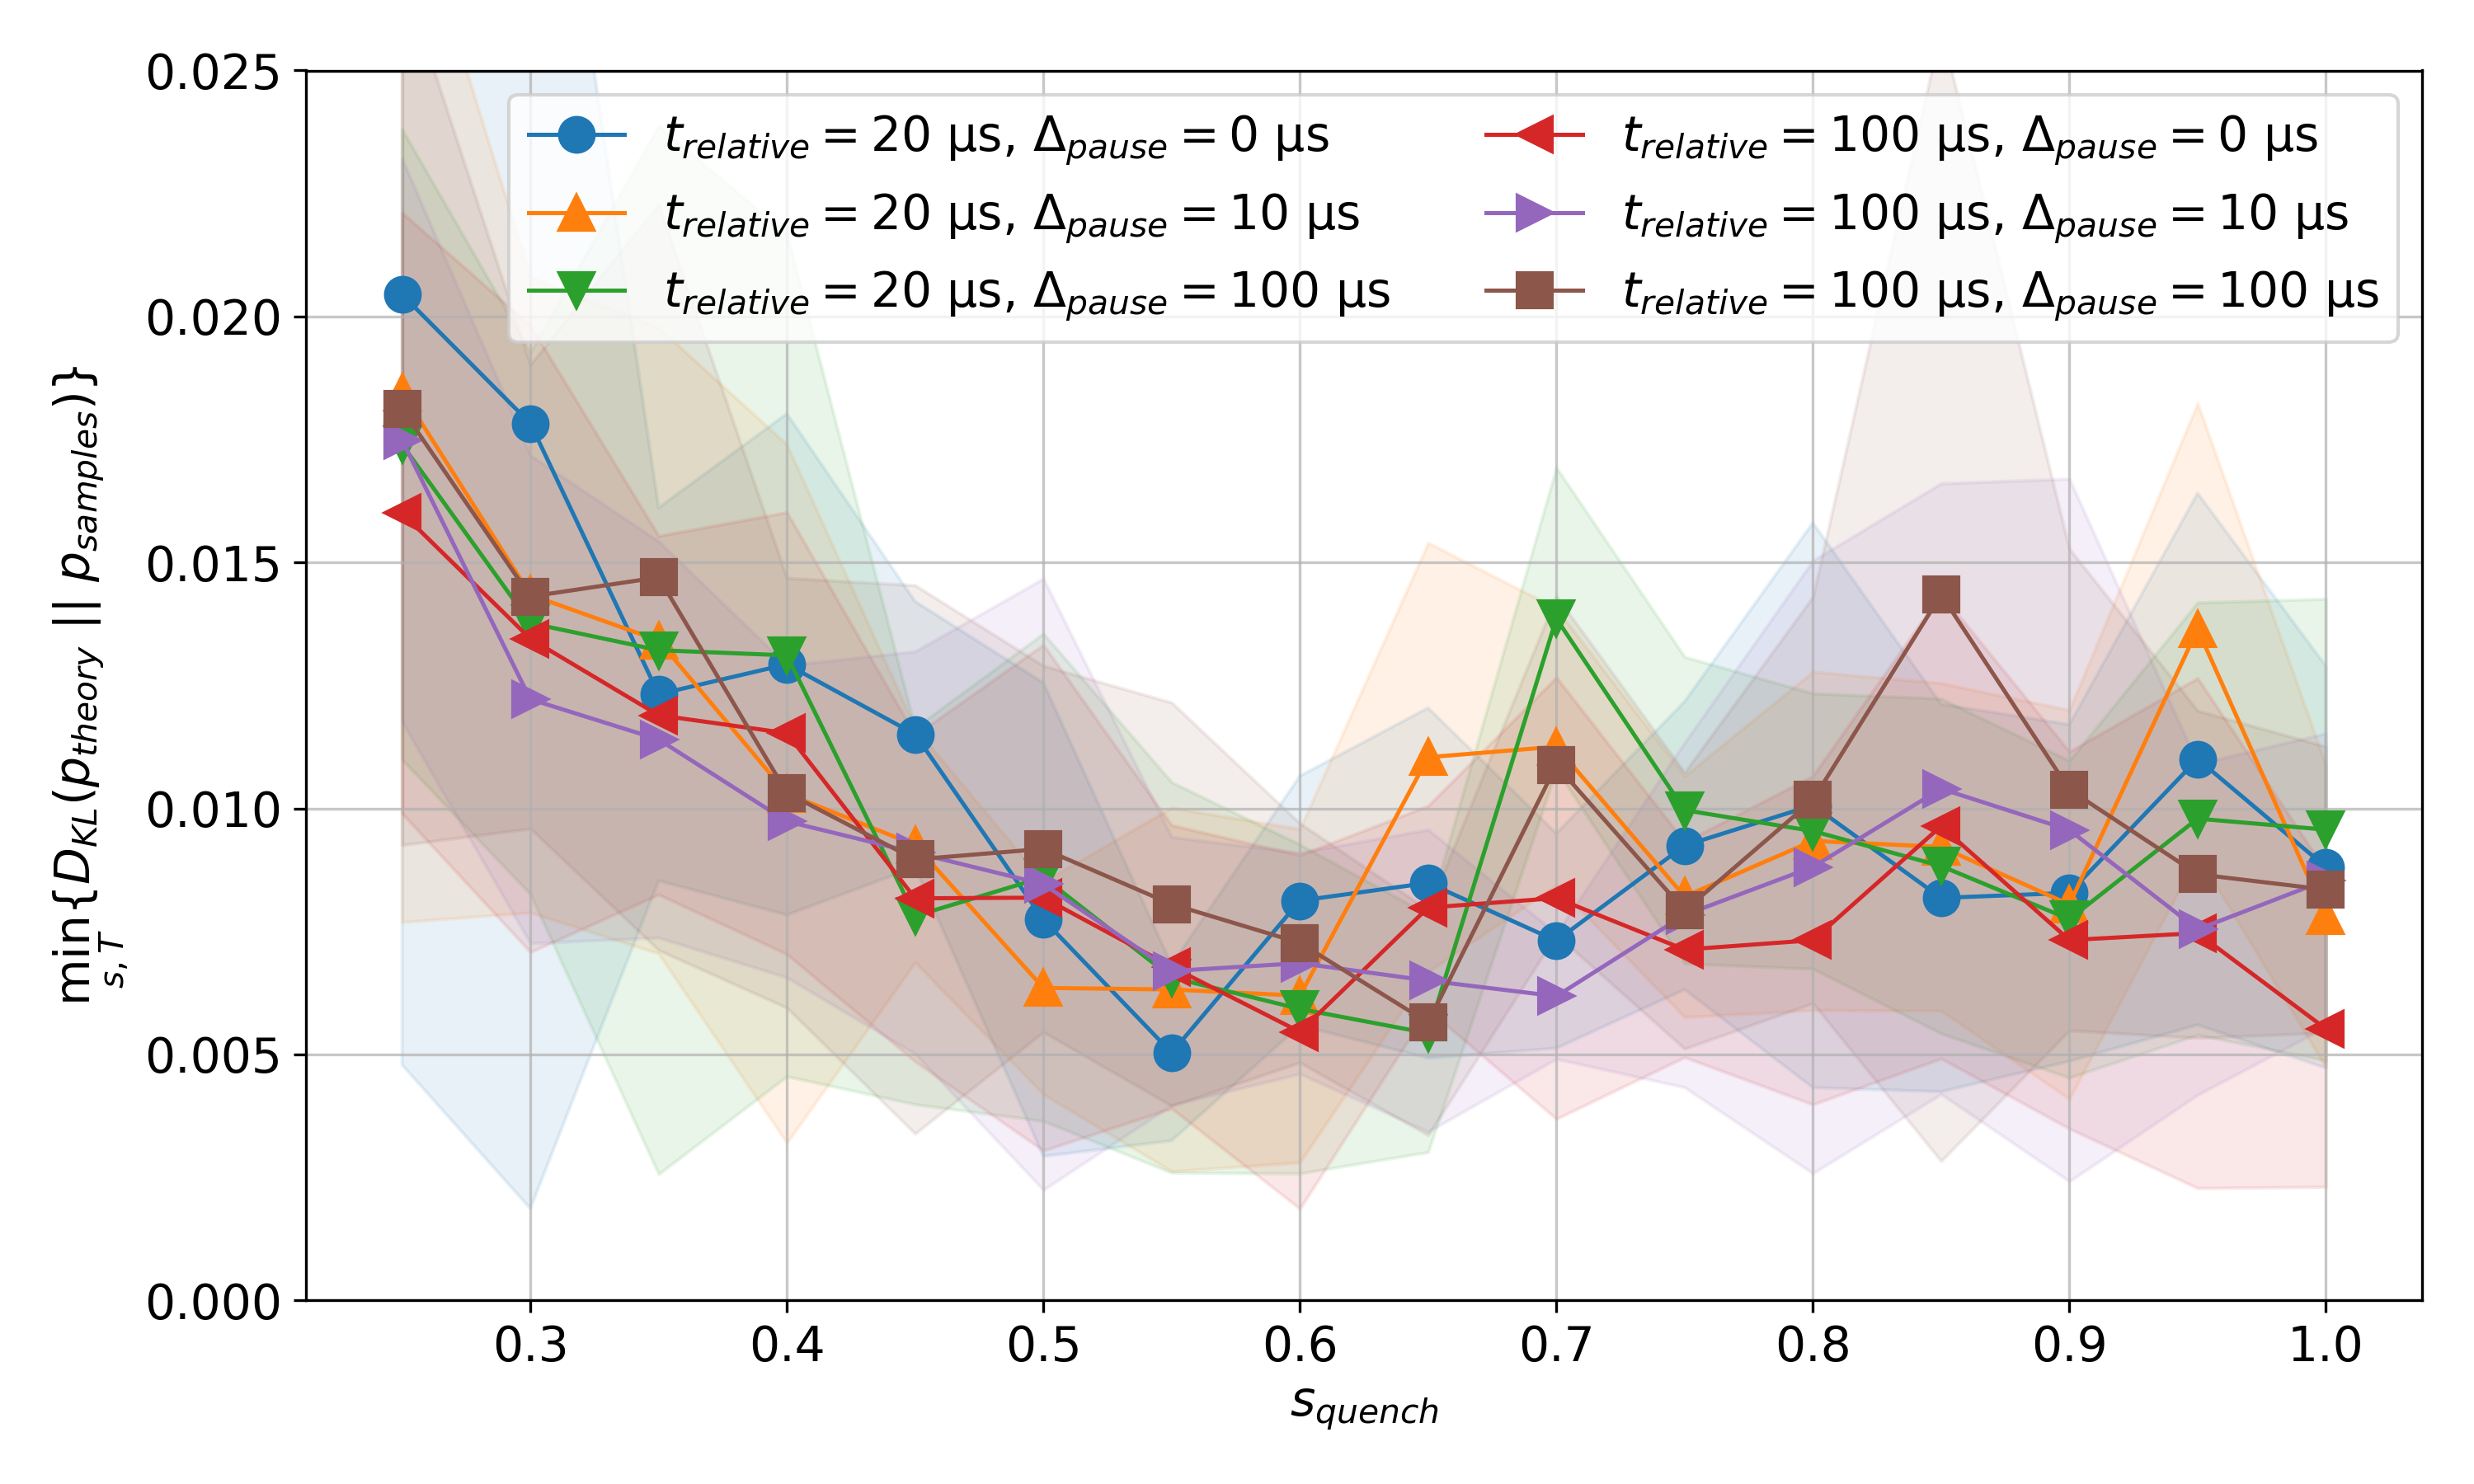
\includegraphics[width=1\linewidth]{qbm/8x4/exact_analysis/config_05/embedding_10/kl_divergence_mins.png}
    \end{figure}
\end{frame}

\begin{frame}
    \frametitle{12-Qubit Autoencoder}
    Trained a quantum restricted Boltzmann machine via the log-likelihood lower bound maximization method (BQRBM) using both a simulation and the D-Wave Advantage 4.1.
    \begin{itemize}
        \item Data set consisted of 1500 samples, 1000 from a \( \mathcal{N}(-2, 1) \) distribution and 500 from a \( \mathcal{N}(3, 1) \) distribution.
        \item 8 visible and 4 hidden units.
        \item Mini-batch size of 10.
        \item \( s^* = 1 \) (reduced the problem to a RBM trained with quantum assistance).
        \item Learning rate held constant at 0.1 for first 50 epochs, then decayed by half every 10 epochs for the remaineder of the training.
    \end{itemize}
\end{frame}

\begin{frame}
    \frametitle{Distribution}
    \begin{figure}
        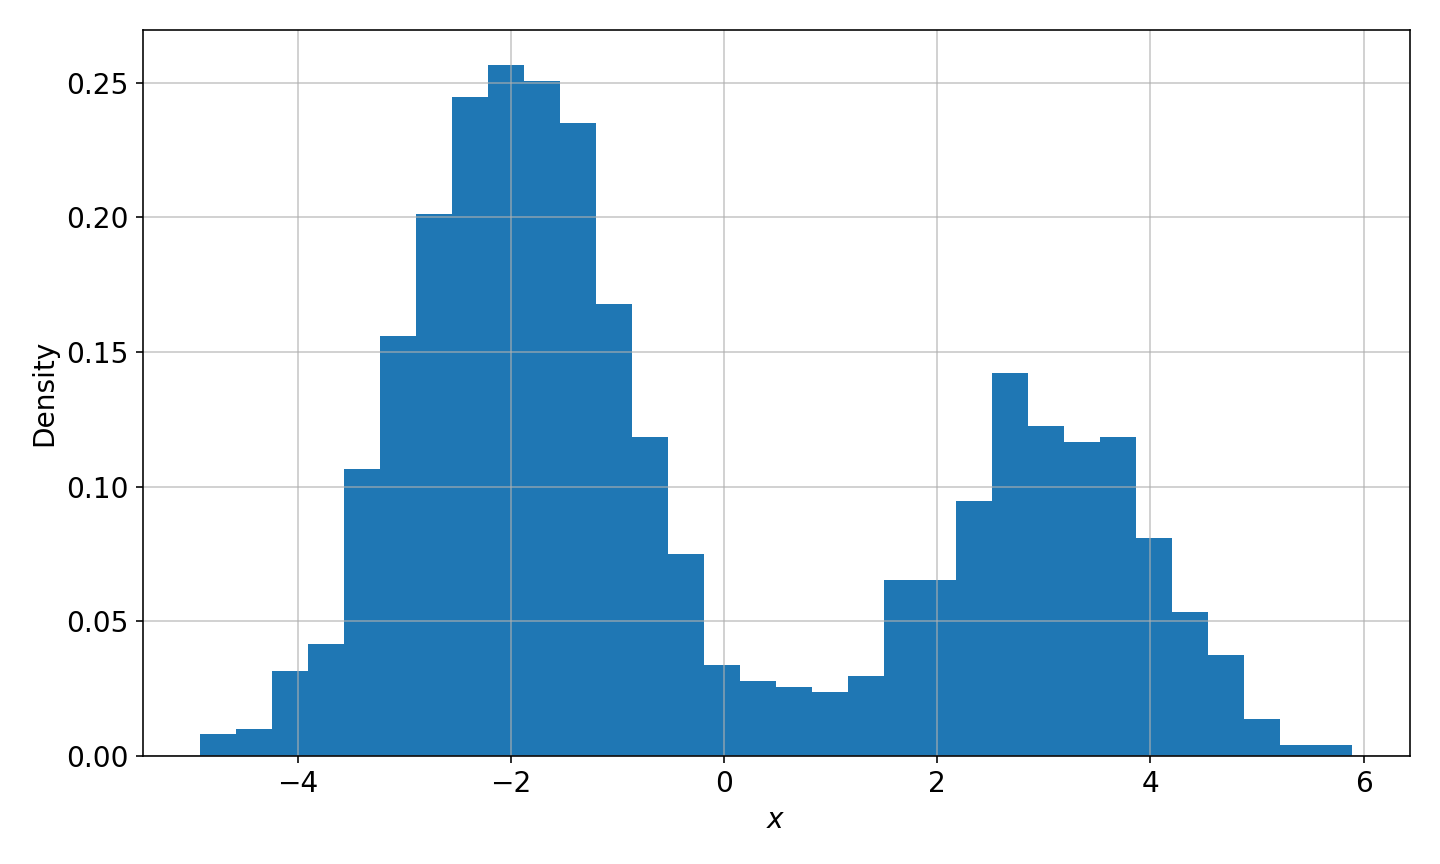
\includegraphics[width=1\linewidth]{qbm/8x4/Advantage_system4.1/hist_data.png}
    \end{figure}
\end{frame}

\begin{frame}
    \frametitle{Model Trained Using a Simulation}
    \begin{figure}
        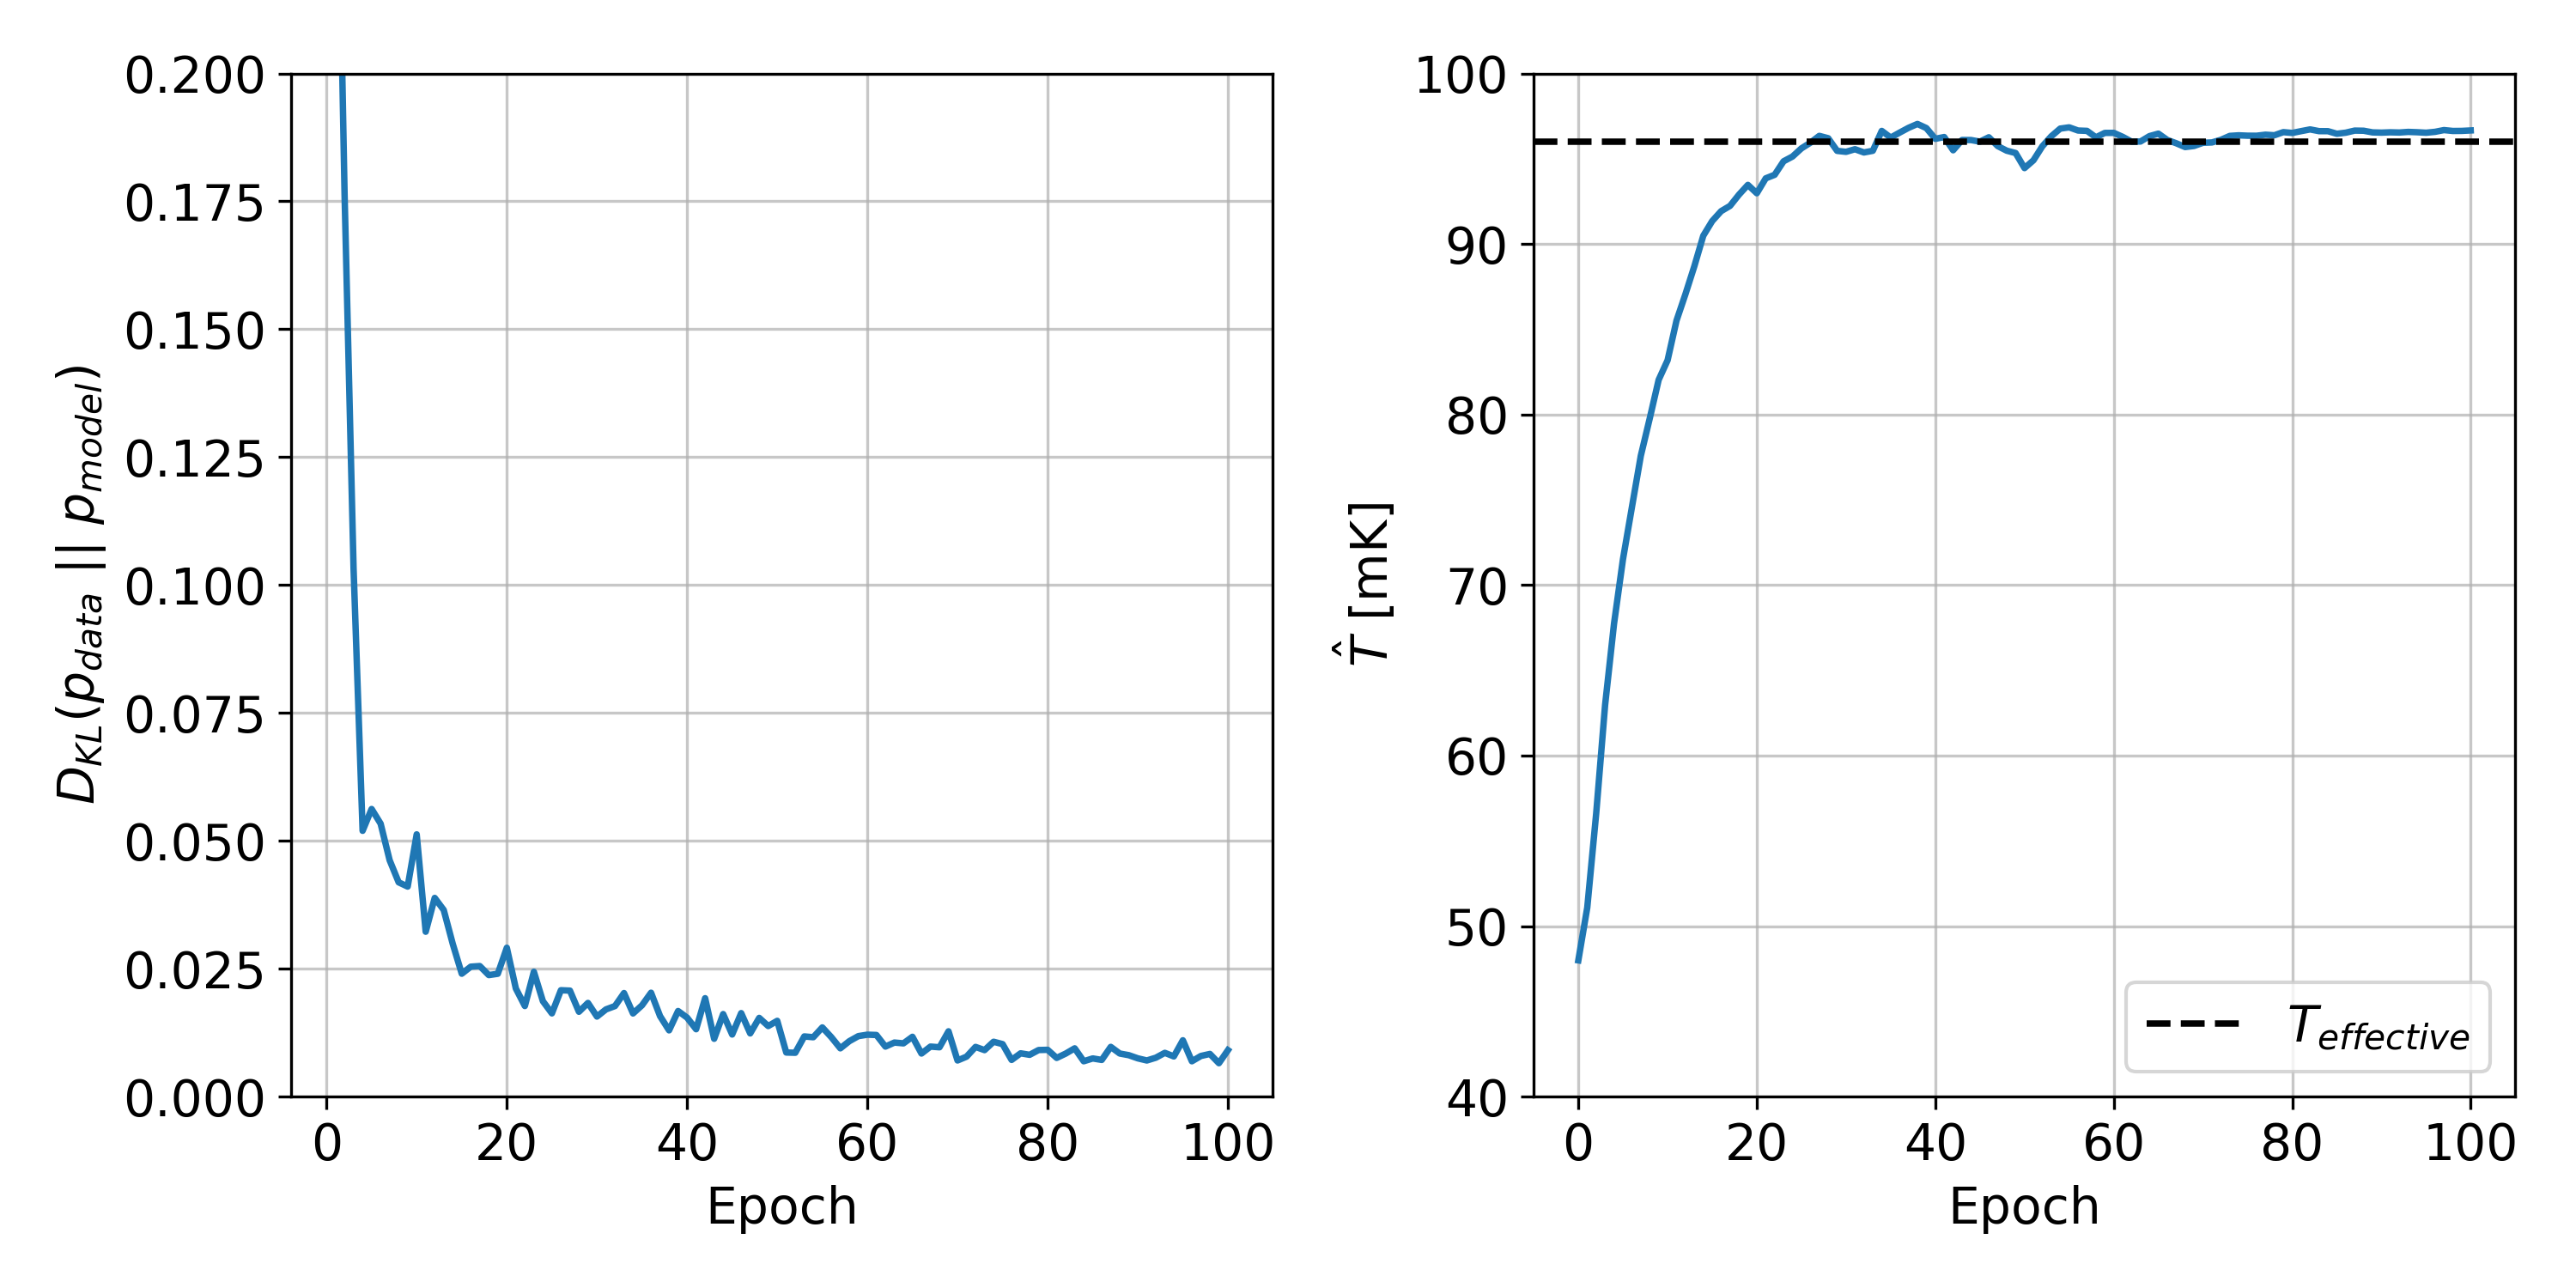
\includegraphics[width=1\linewidth]{qbm/8x4/Advantage_system4.1/train_results_exact.png}
    \end{figure}
\end{frame}

\begin{frame}
    \frametitle{Model Trained Using the Advantage 4.1}
    \begin{figure}
        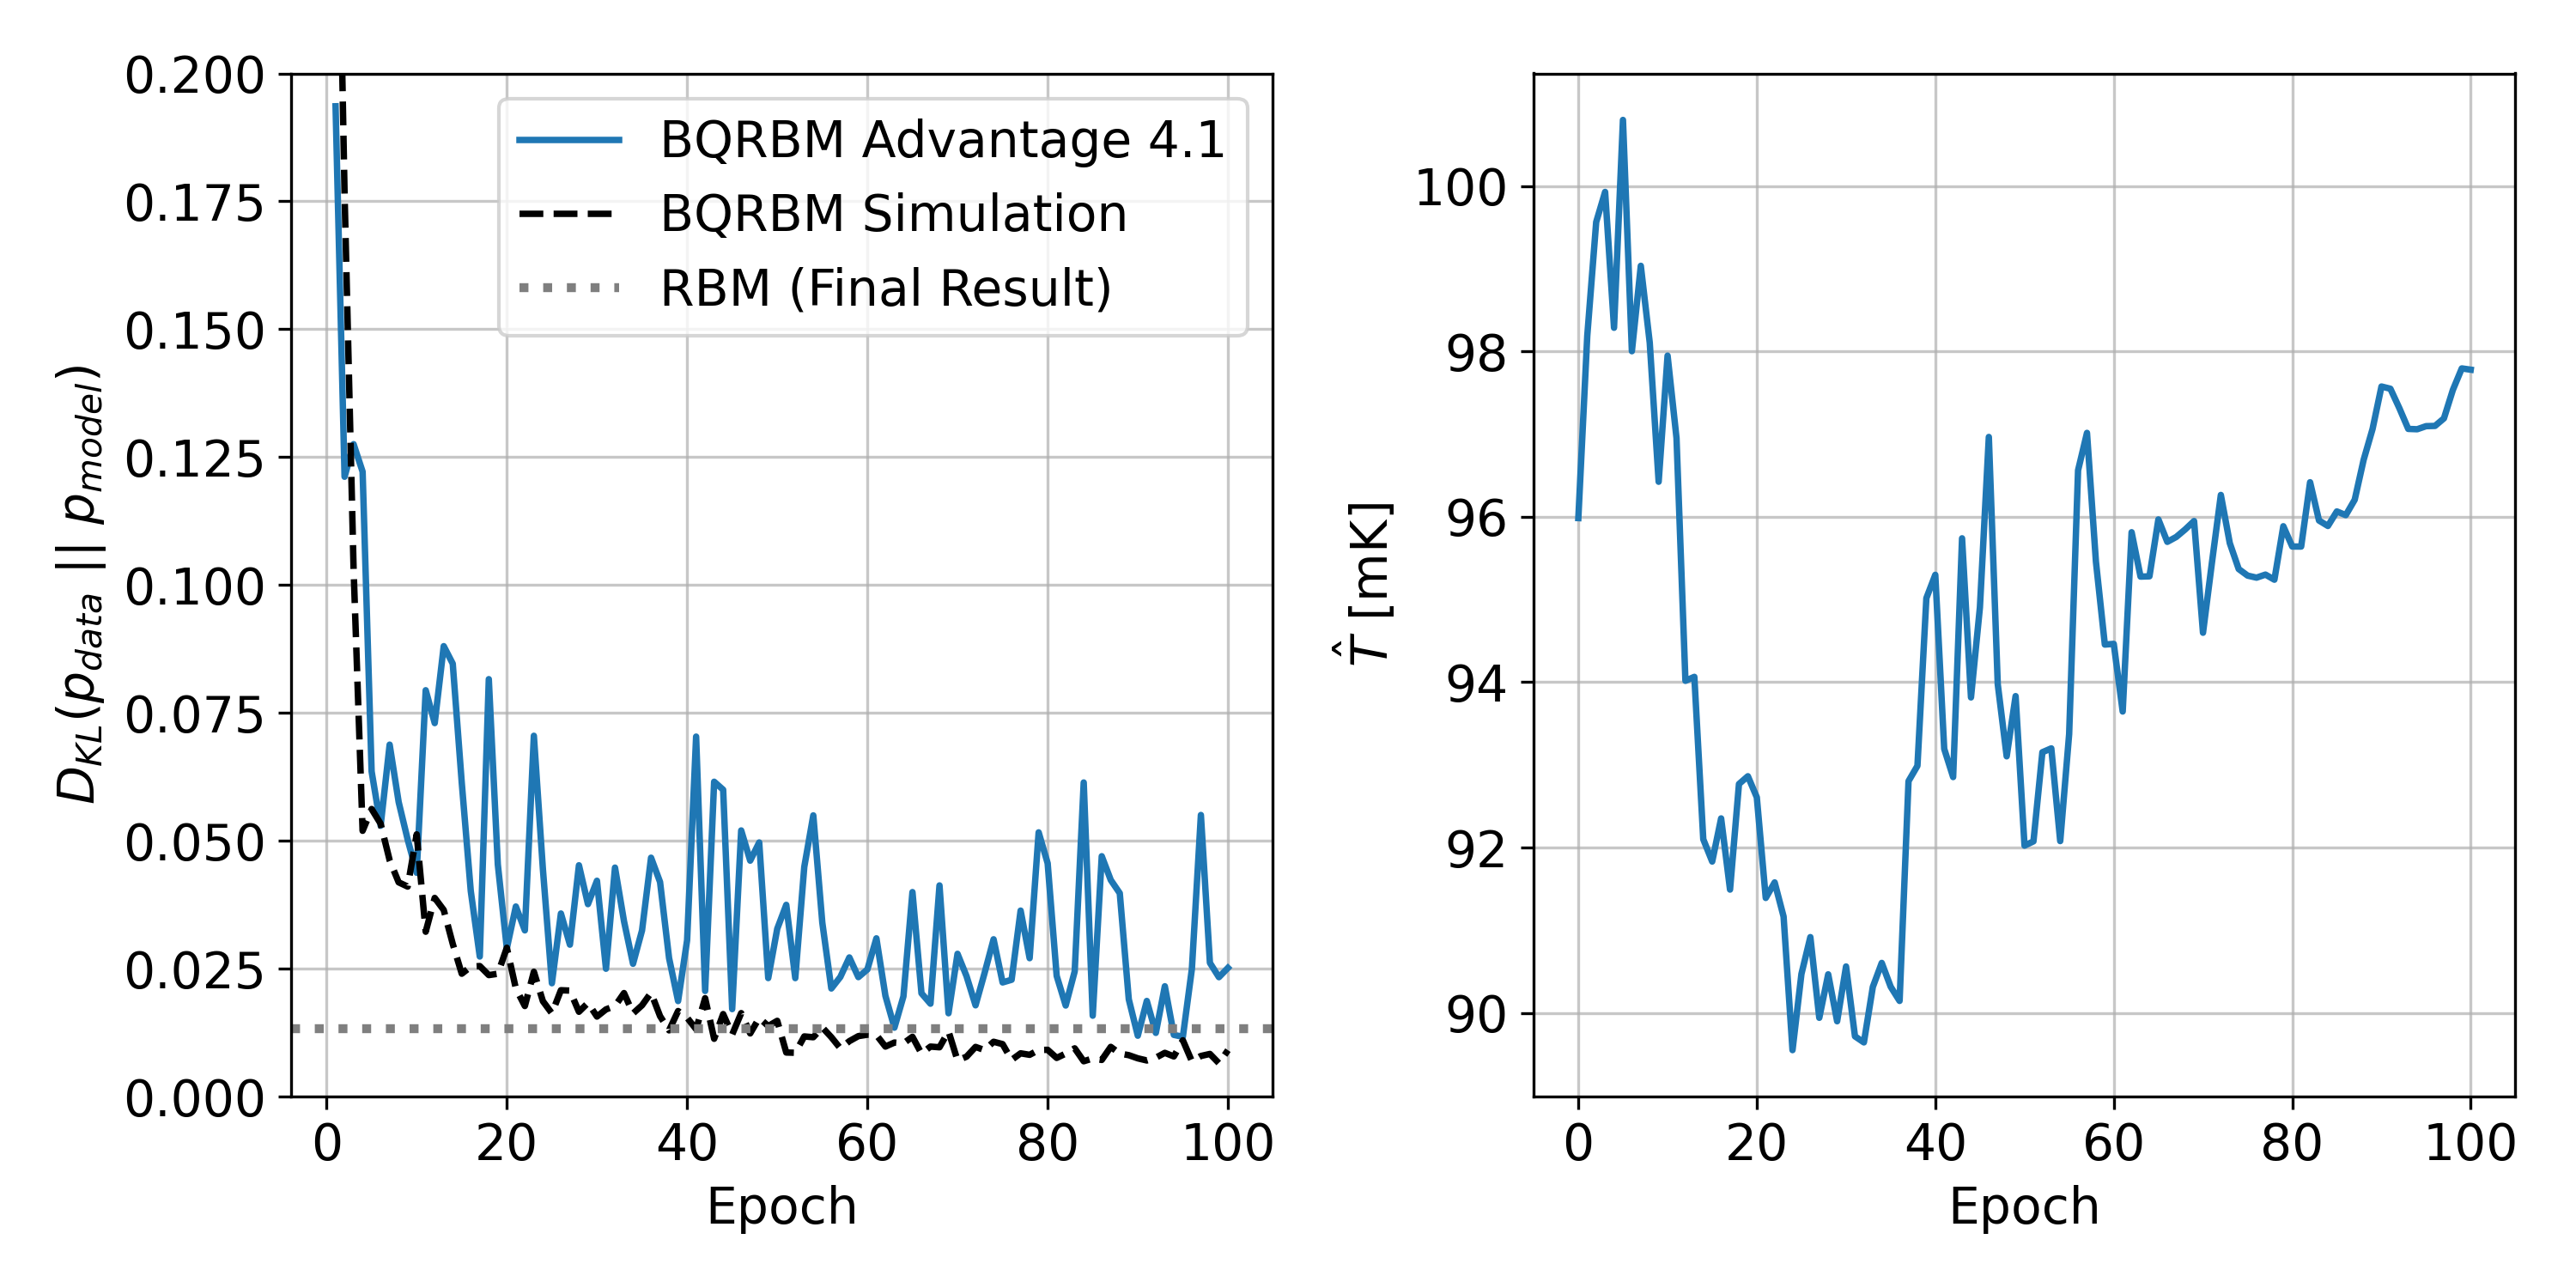
\includegraphics[width=1\linewidth]{qbm/8x4/Advantage_system4.1/train_results_annealer.png}
    \end{figure}
\end{frame}

\begin{frame}
    \frametitle{QQ Plots}
    \begin{figure}
        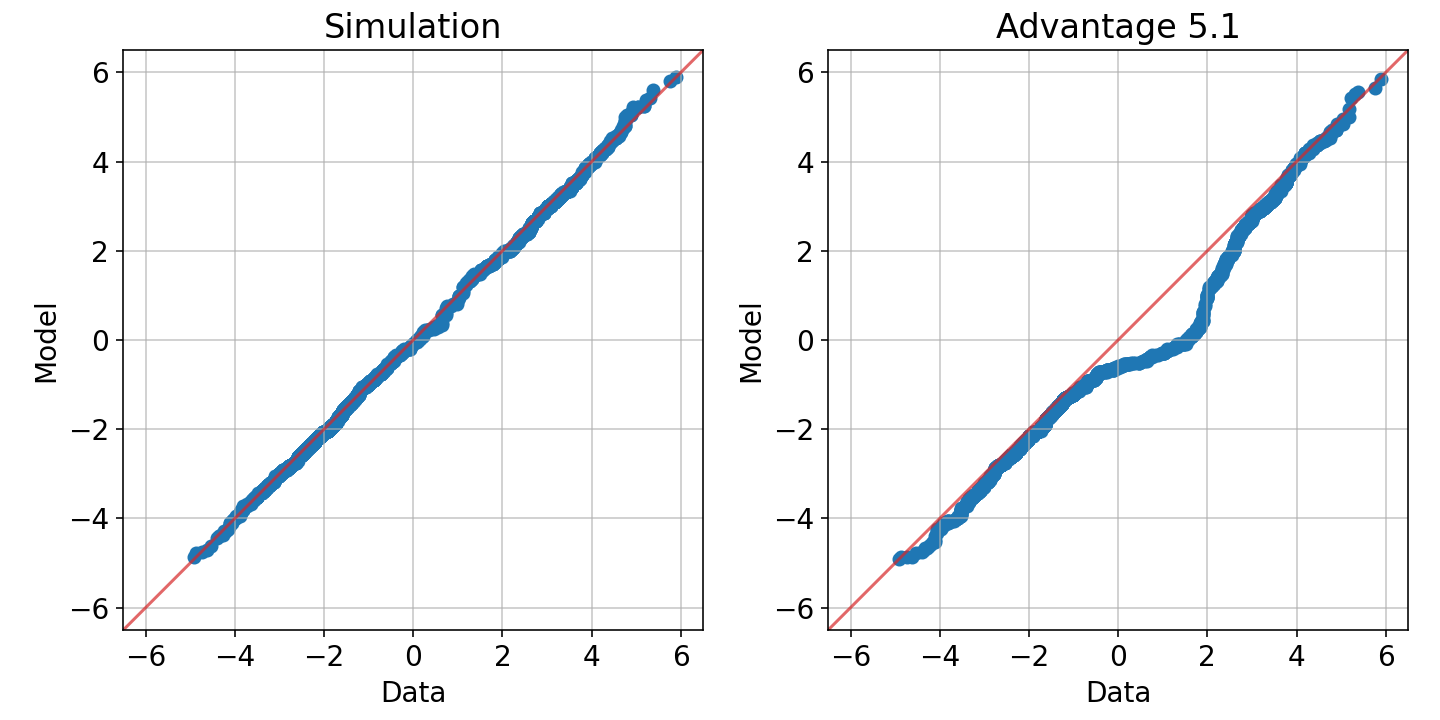
\includegraphics[width=1\linewidth]{qbm/8x4/Advantage_system4.1/qq_comparison.png}
    \end{figure}
\end{frame}

\begin{frame}
    \frametitle{Verifying the Learned Effective Temperature}
    \begin{figure}
        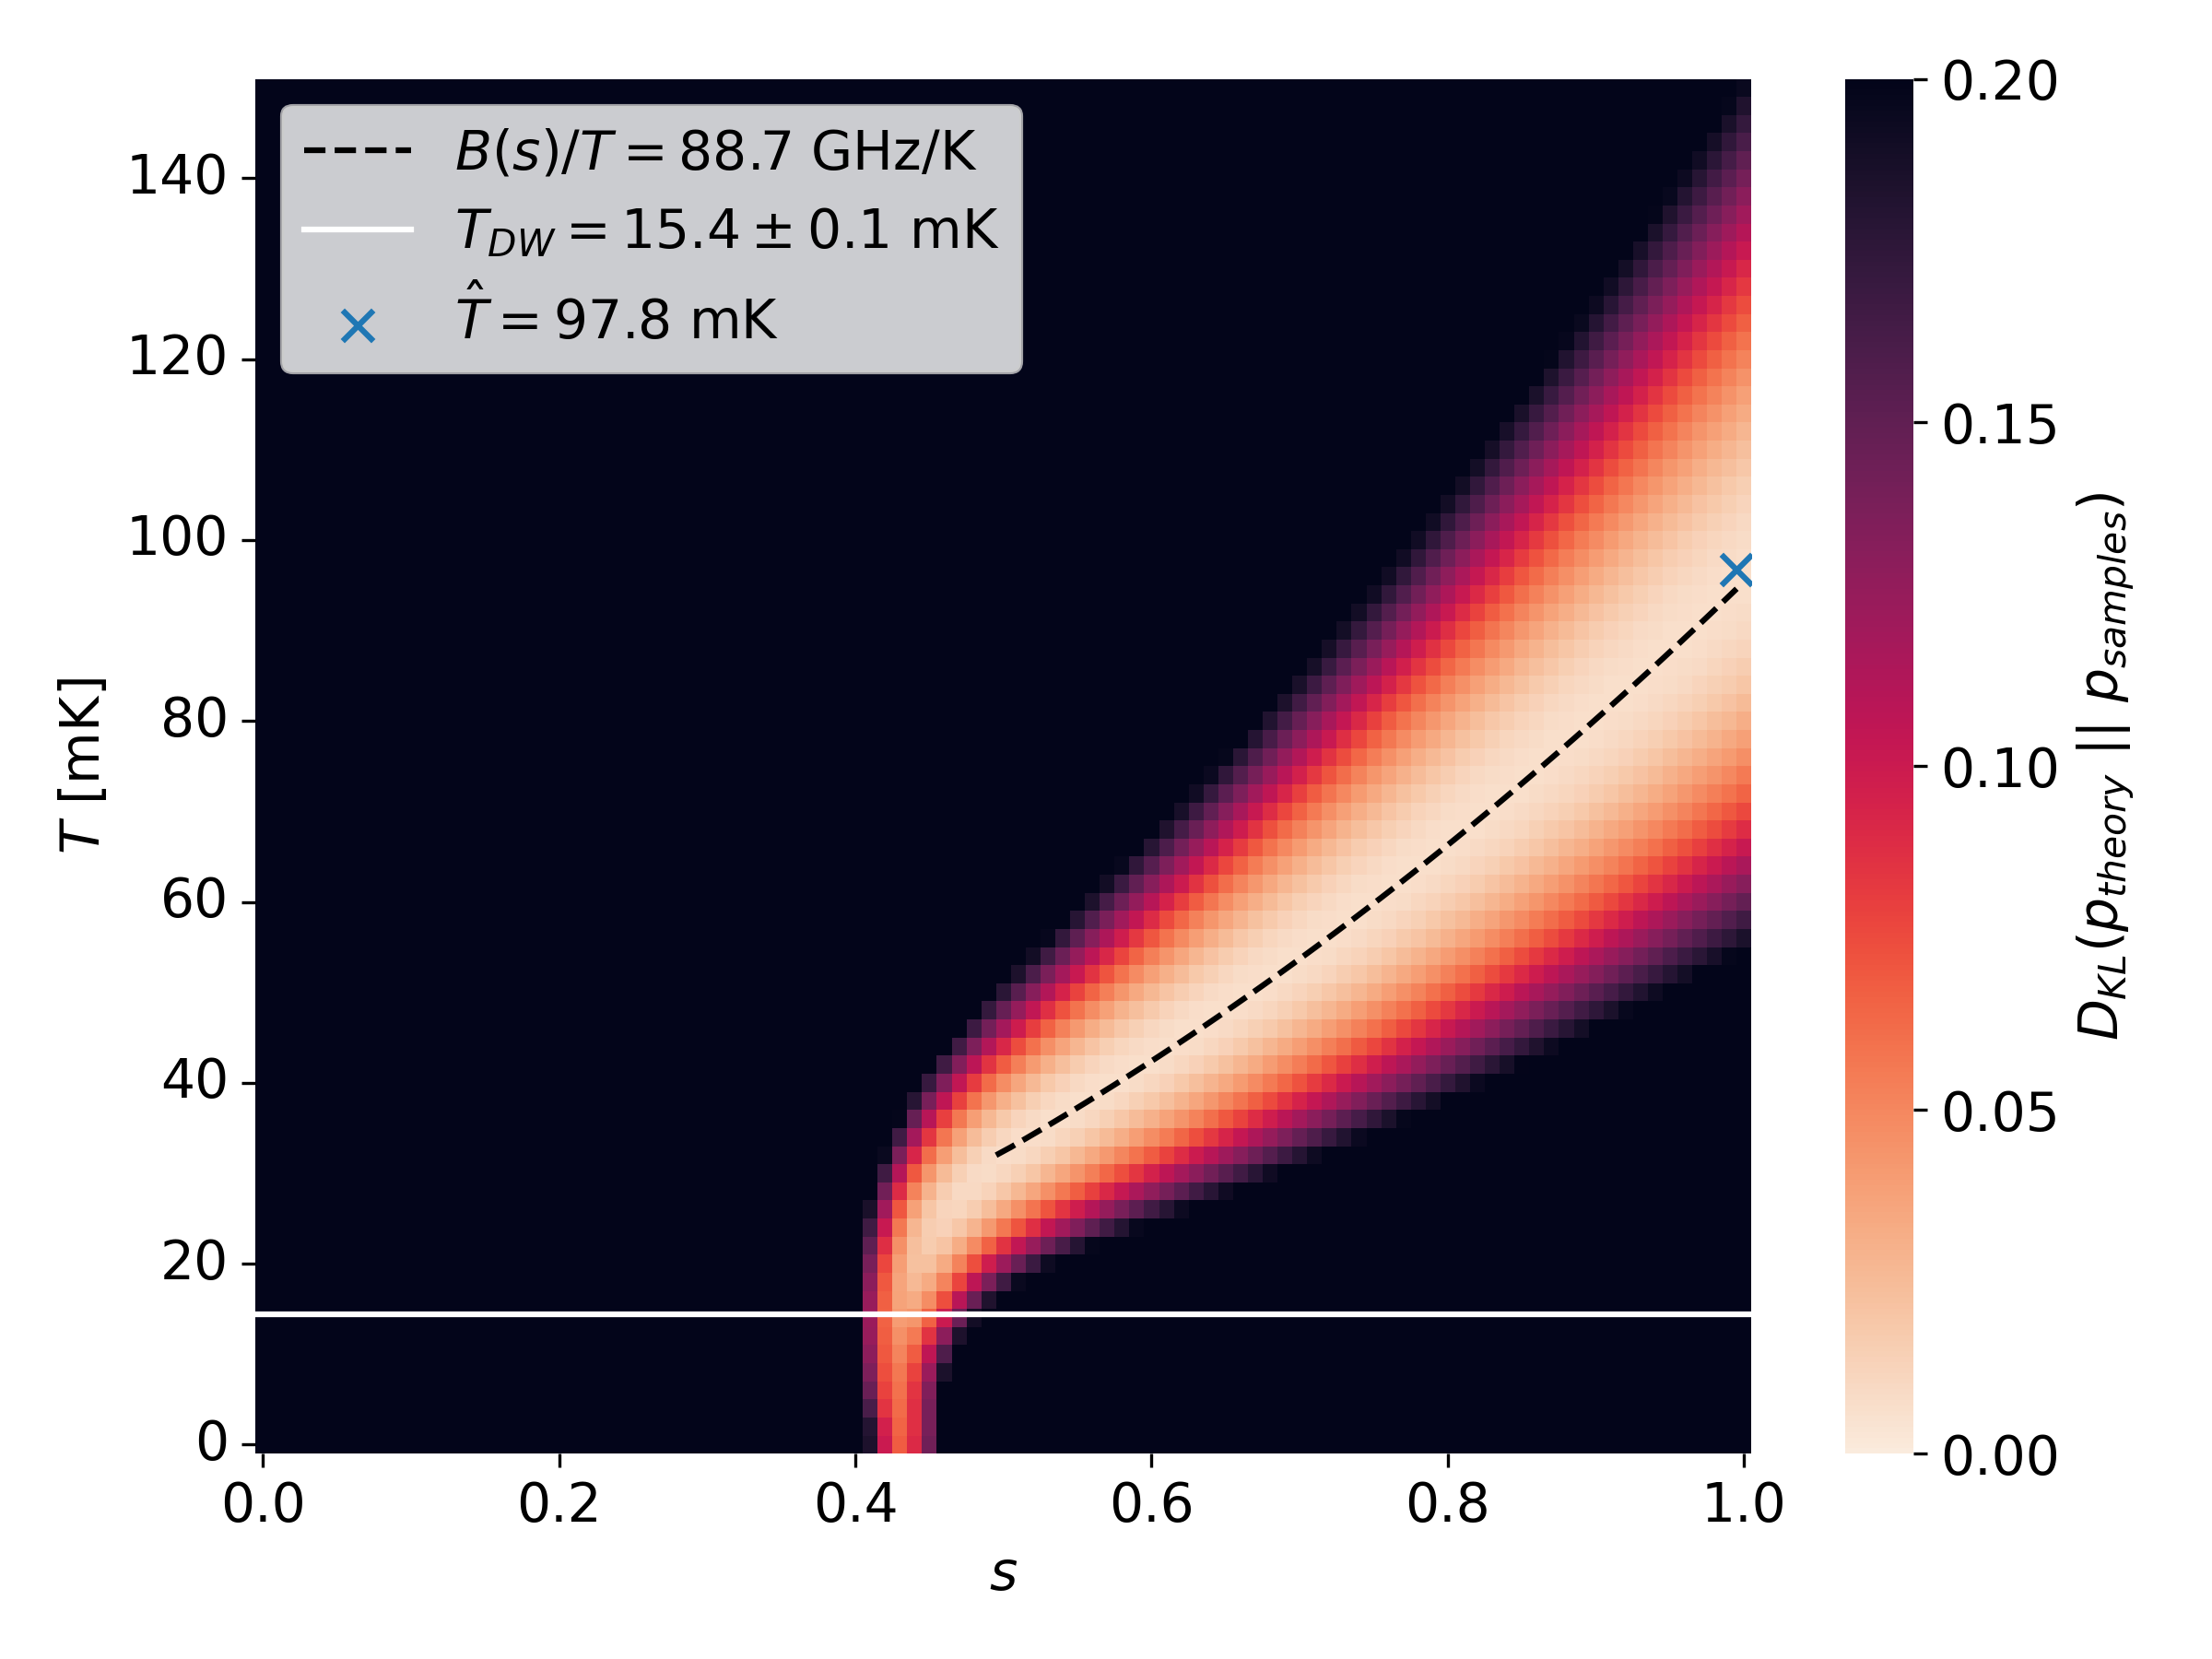
\includegraphics[width=0.9\linewidth]{qbm/8x4/Advantage_system4.1/effective_temperature.png}
    \end{figure}
\end{frame}

\subsection{The Quantum Market Generator}
\begin{frame}
    \frametitle{The Quantum Market Generator}
    Trained a quantum restricted Boltzmann machine via the log-likelihood lower bound maximization method (BQRBM) using both a simulation and the D-Wave Advantage 4.1.
    \begin{itemize}
        \item 64 visible and 30 hidden units.
        \item Mini-batch size of 10.
        \item \( s^* = 1 \) (reduced the problem to a RBM trained with quantum assistance).
        \item Learning rate held constant at 0.02 (0.01 for effective inverse temperature).
    \end{itemize}
\end{frame}

\begin{frame}
    \frametitle{Relative Chain Strength Scan}
    \begin{figure}
        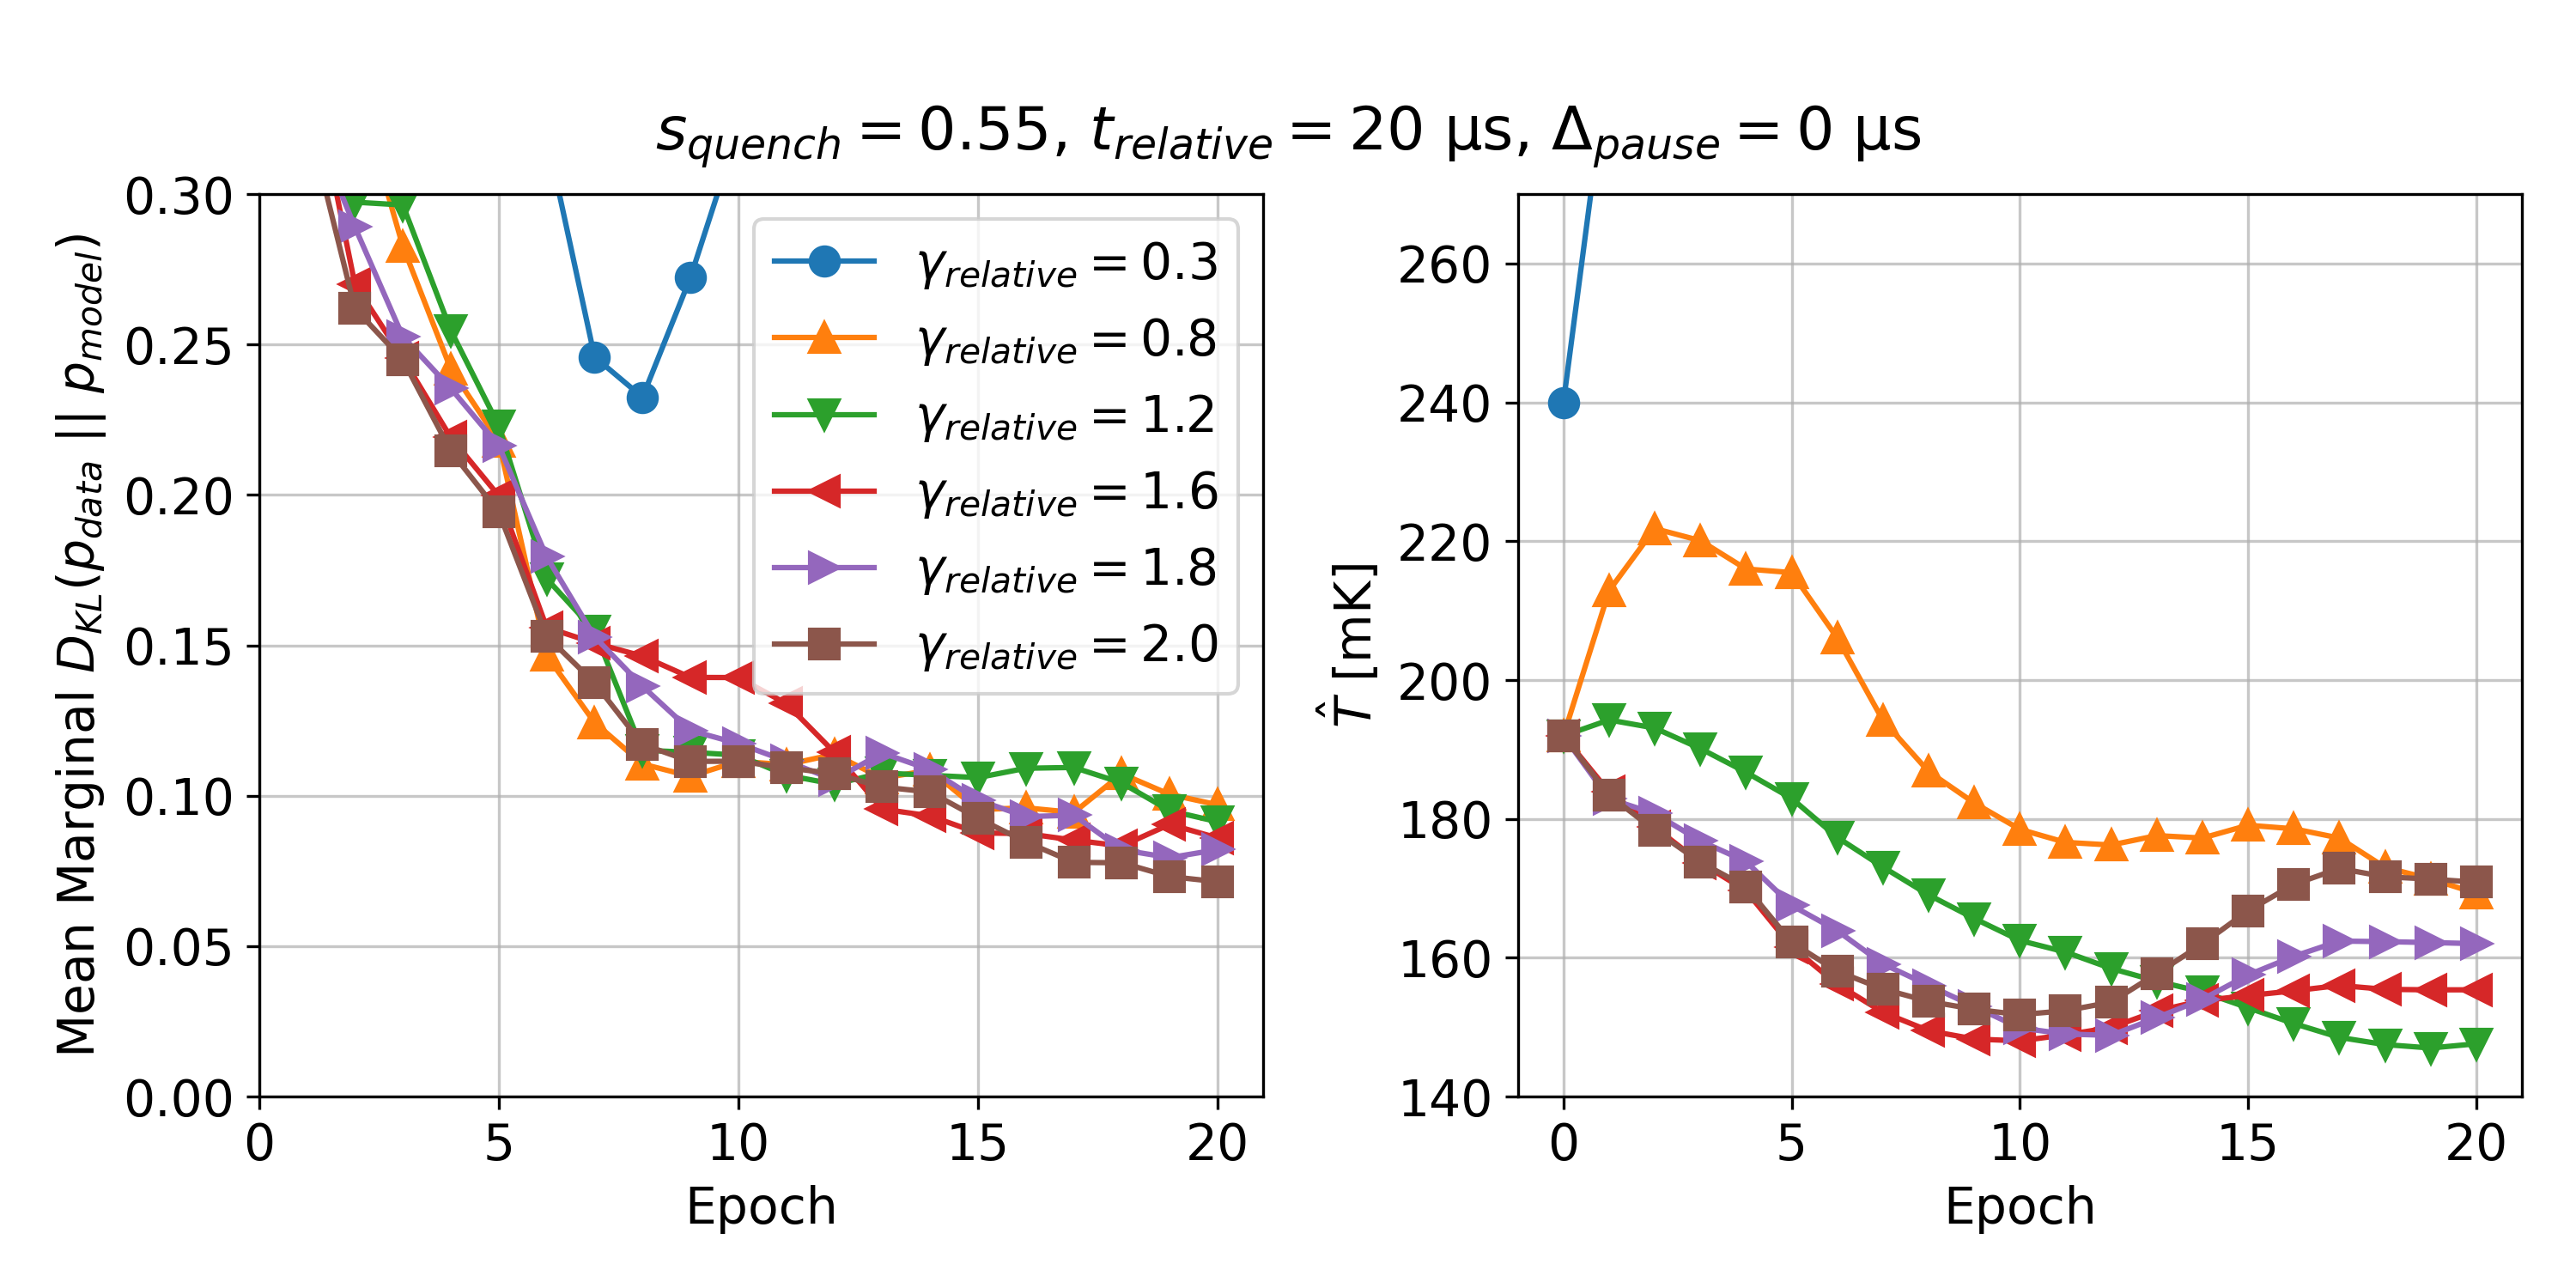
\includegraphics[width=1\linewidth]{qbm/log_returns/rcs_comparison.png}
    \end{figure}
\end{frame}

\begin{frame}
    \frametitle{\( \squench \) Scan}
    \begin{figure}
        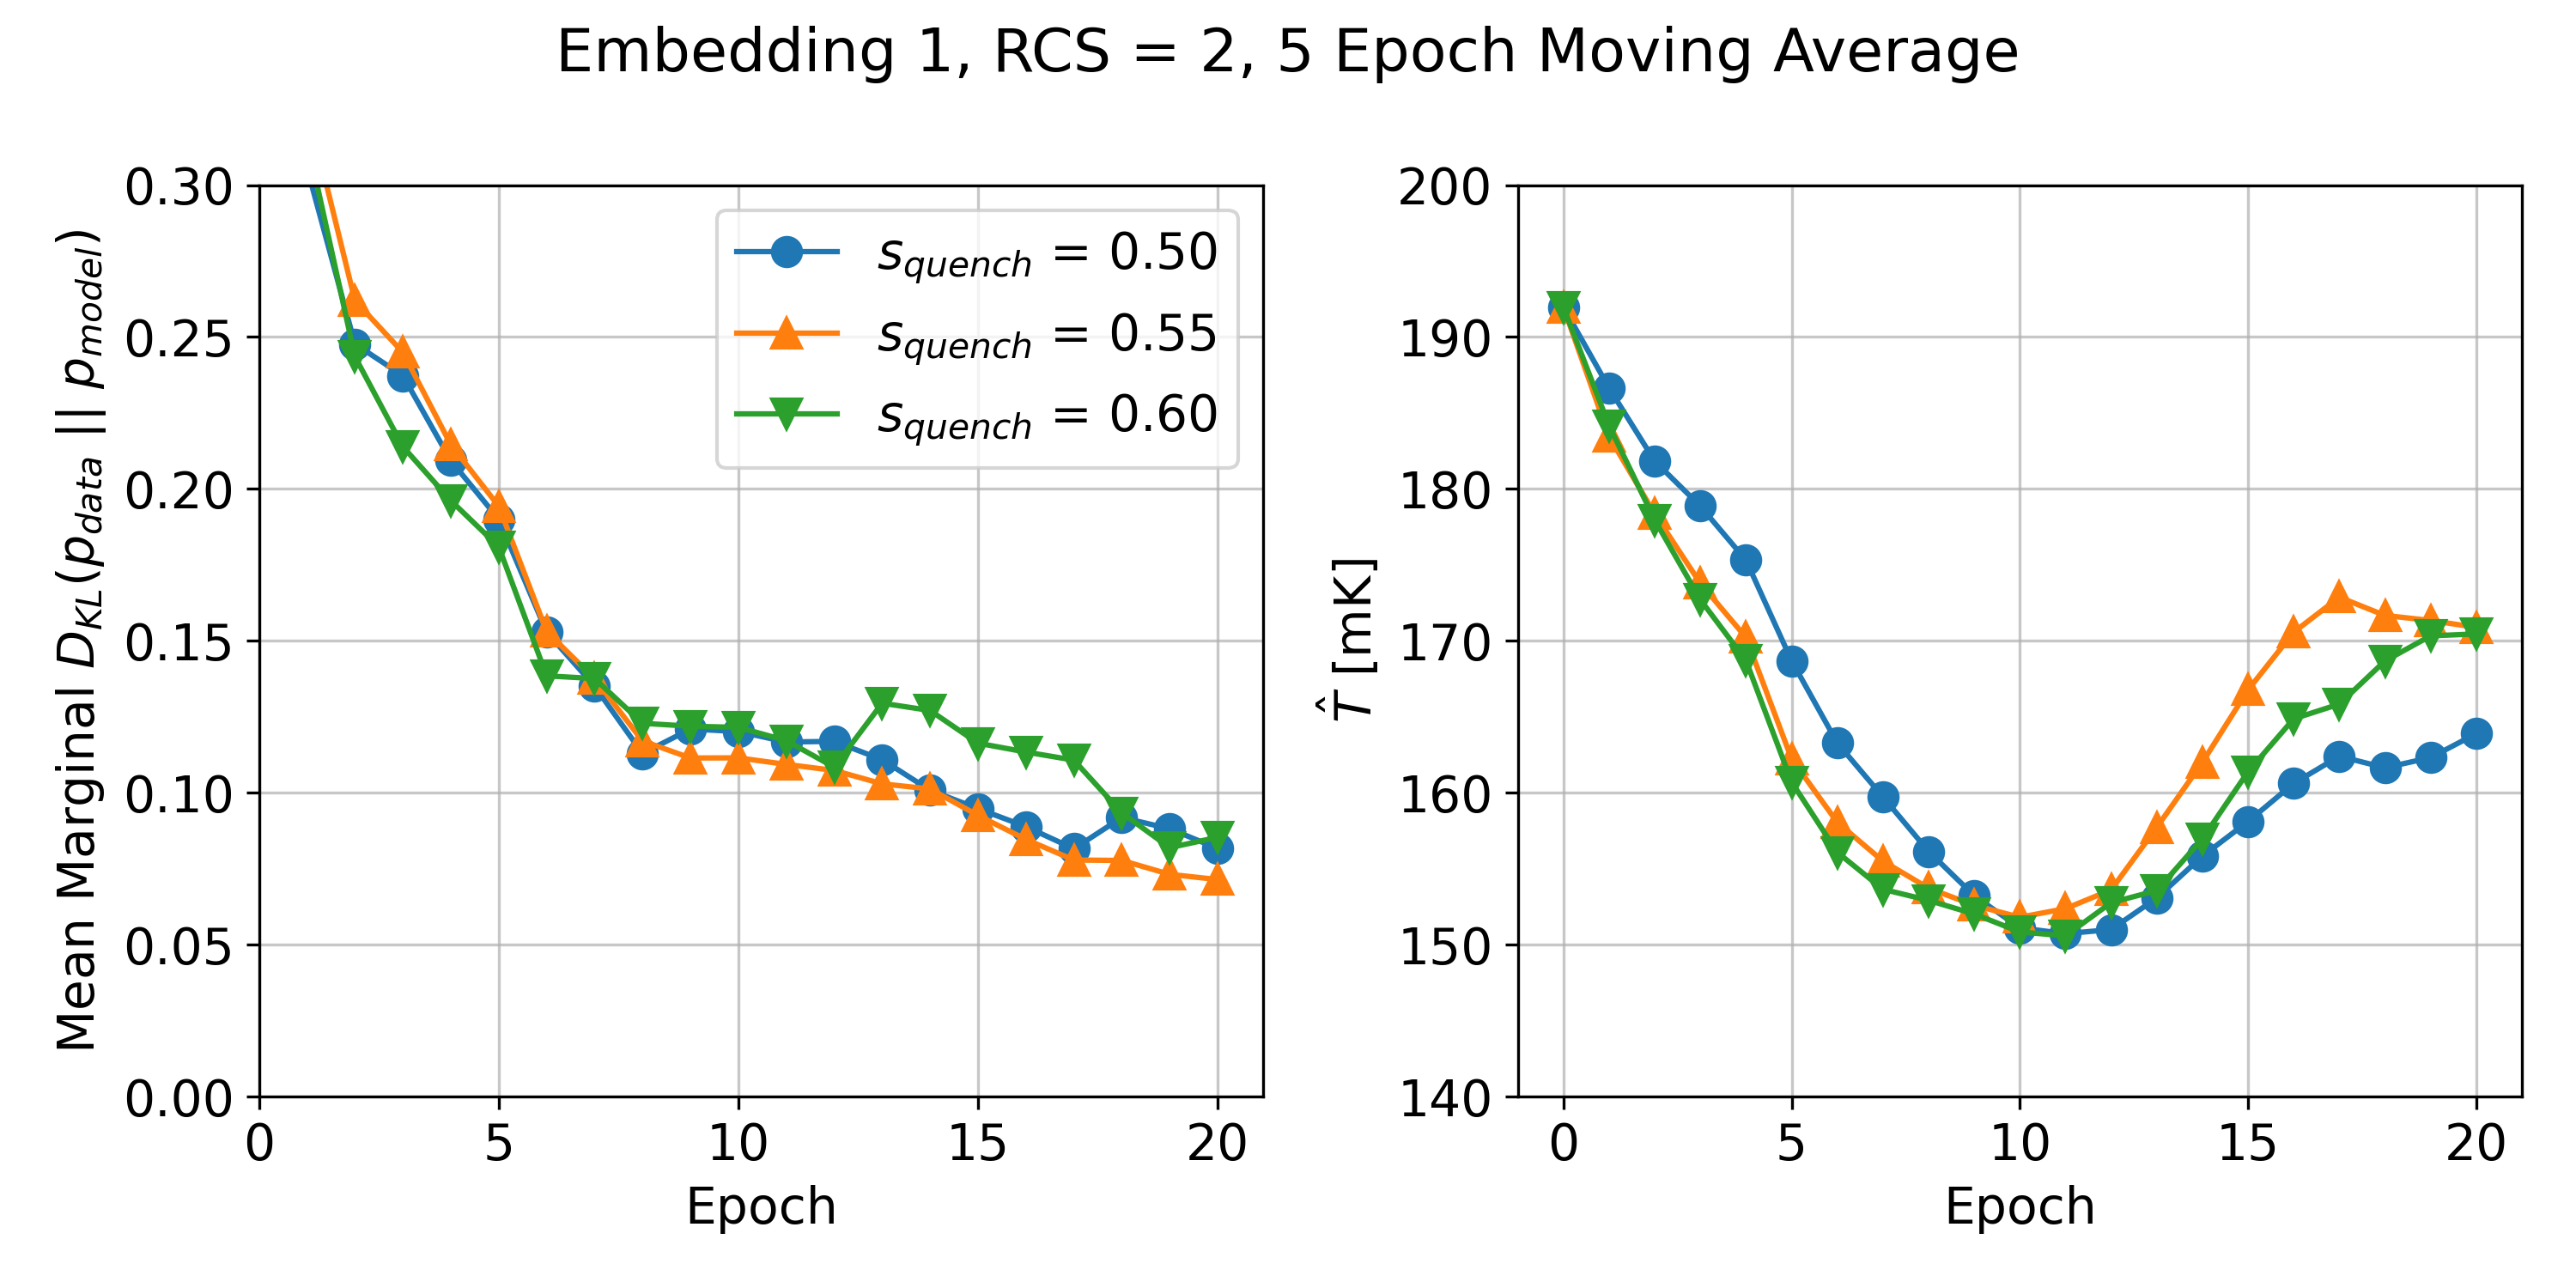
\includegraphics[width=1\linewidth]{qbm/log_returns/s_quench_comparison.png}
    \end{figure}
\end{frame}

\begin{frame}
    \frametitle{Embedding Comparison}
    \begin{figure}
        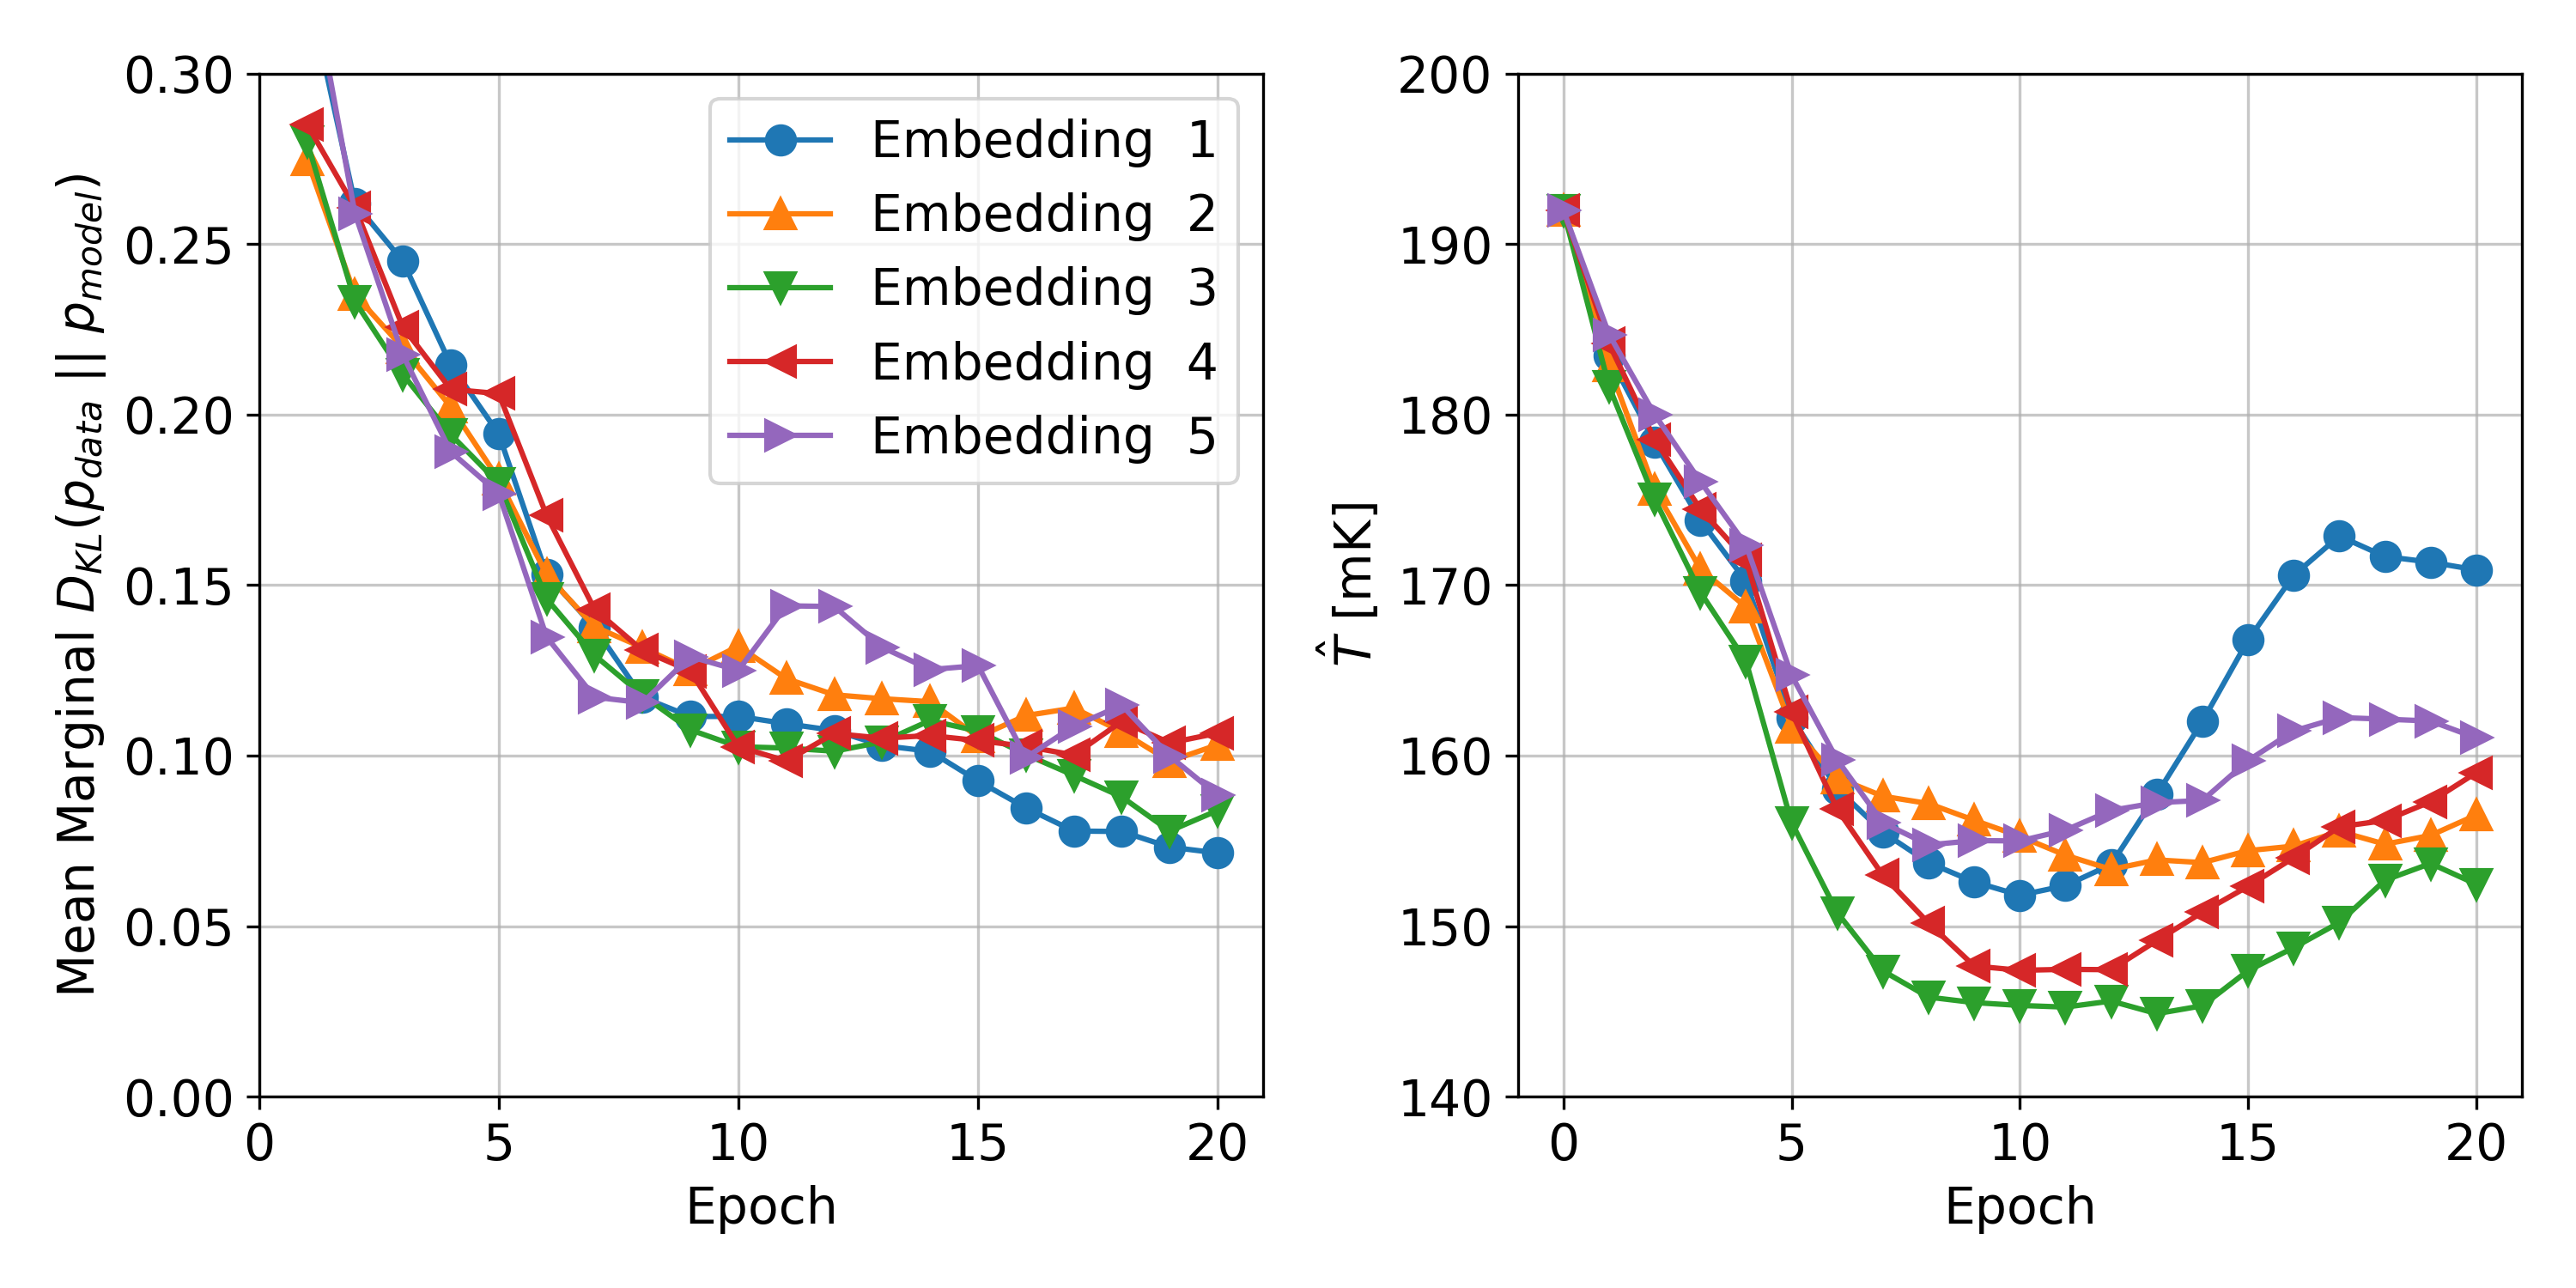
\includegraphics[width=1\linewidth]{qbm/log_returns/embedding_comparison.png}
    \end{figure}
\end{frame}

\begin{frame}
    \frametitle{Training Results}
    \begin{figure}
        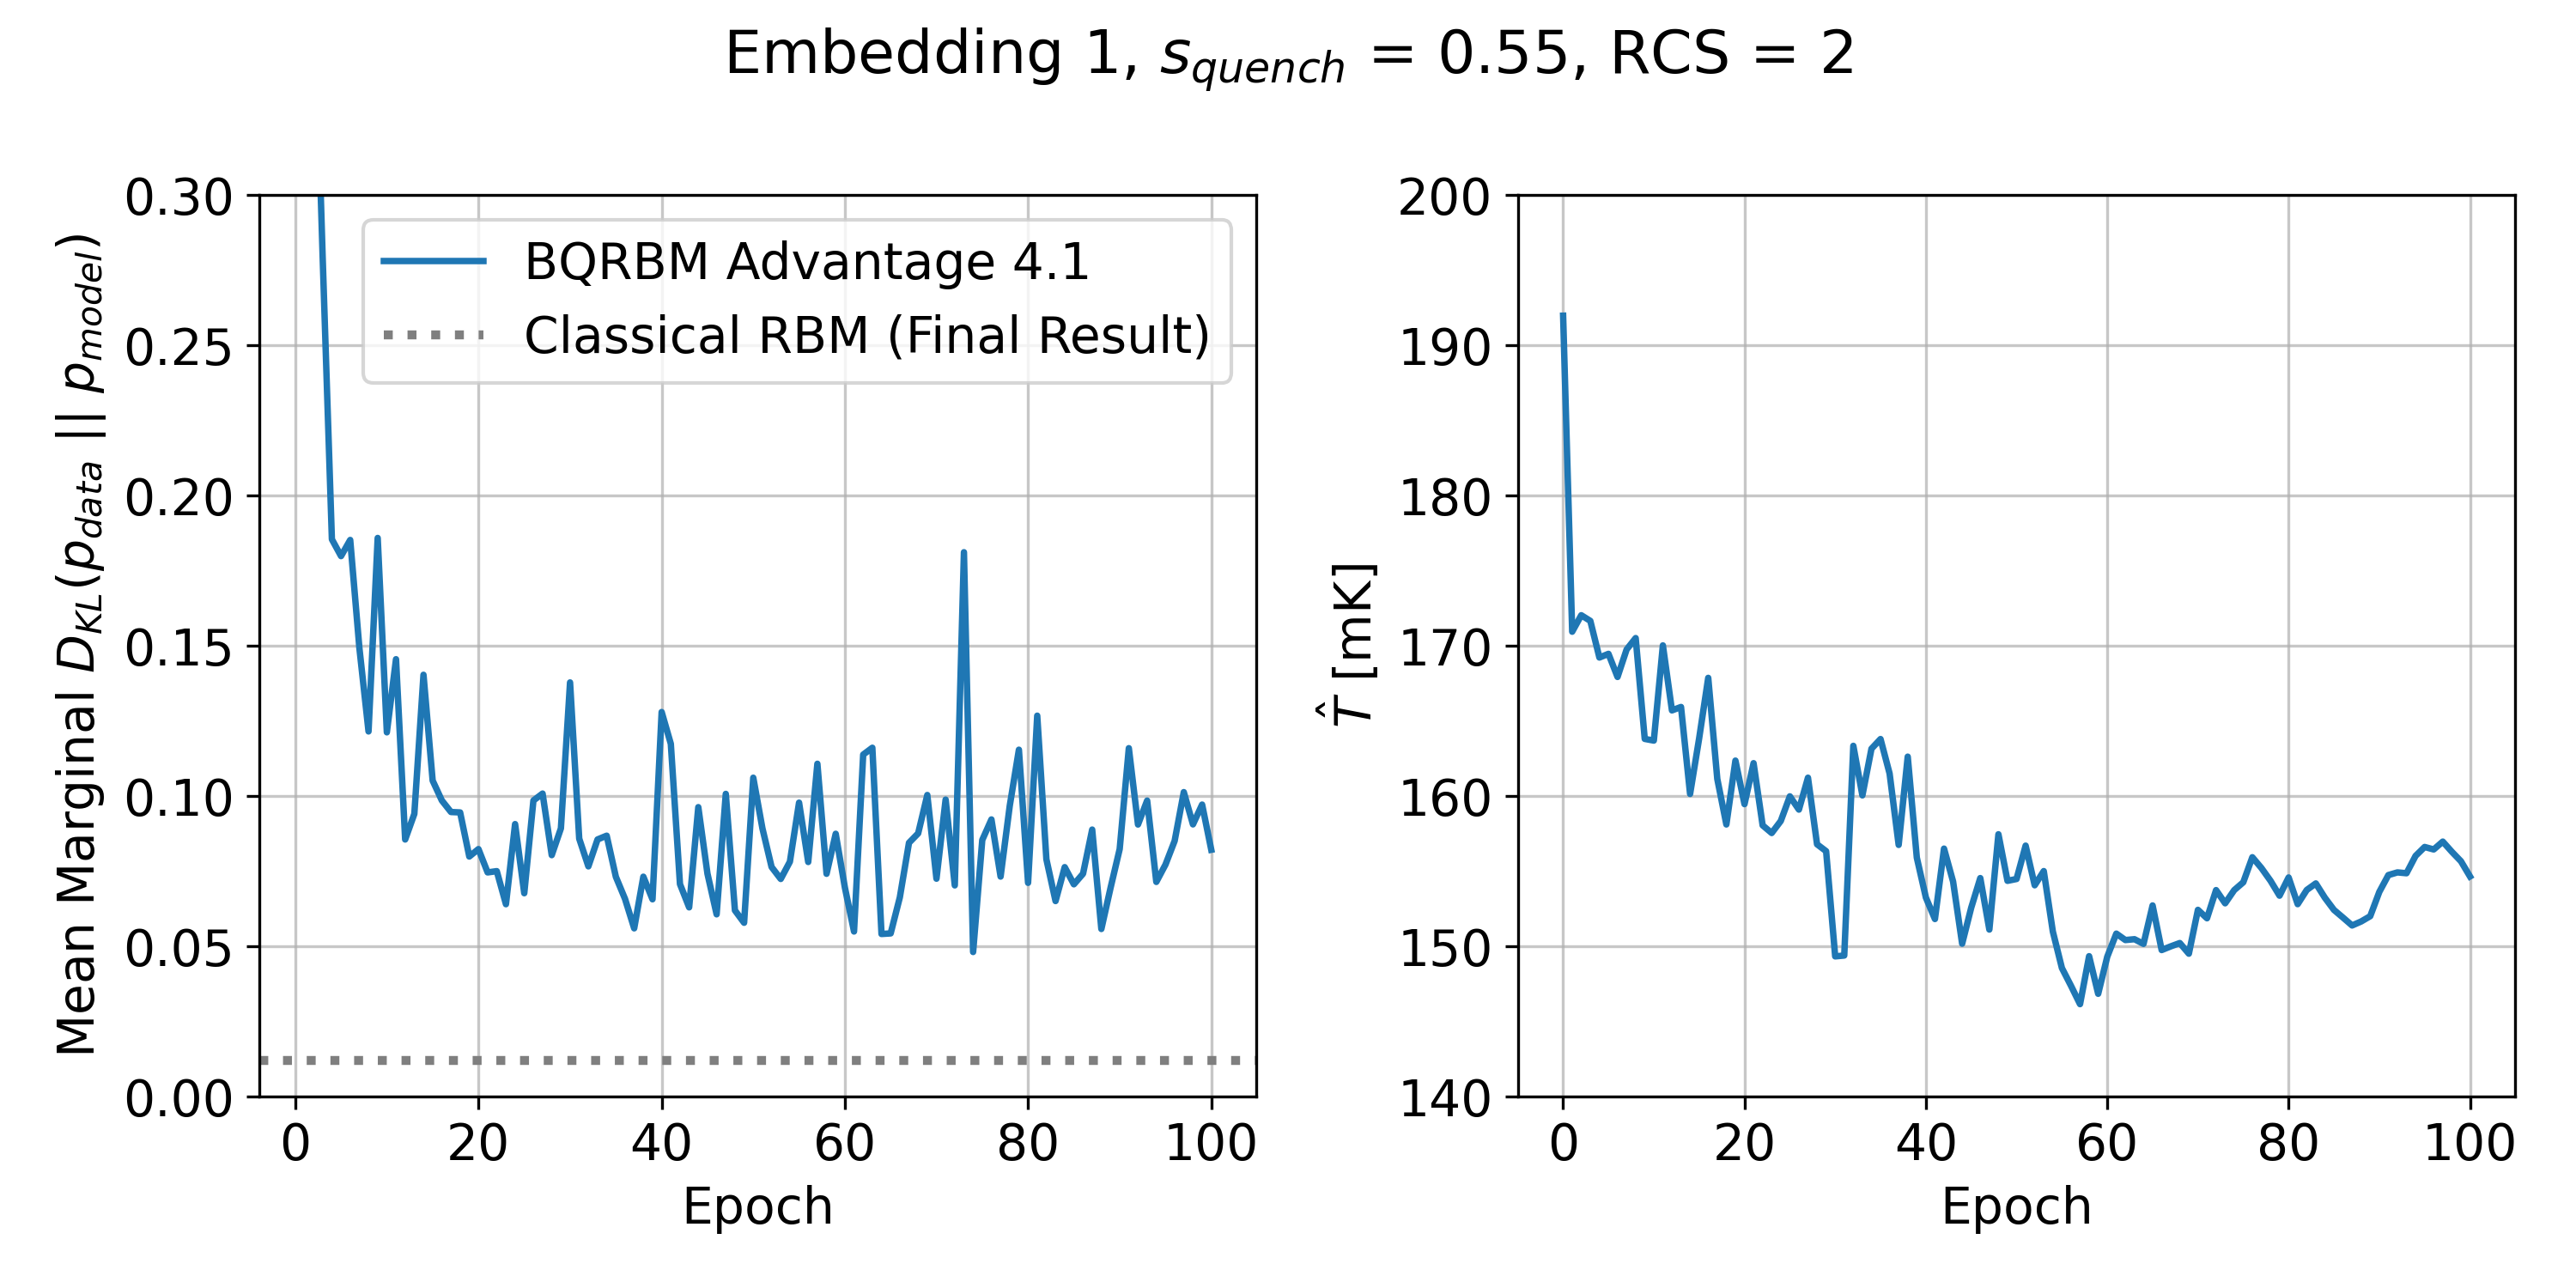
\includegraphics[width=1\linewidth]{qbm/log_returns/full_run.png}
    \end{figure}
\end{frame}

\begin{frame}
    \frametitle{KL Divergences}
    \begin{table}[!htb]
        \centering
        \begin{adjustbox}{max width=\textwidth}
            \input{../../tables/qbm/kl_divergences.tbl}
        \end{adjustbox}
    \end{table}
\end{frame}

%\begin{frame}
    %\frametitle{Correlation Coefficients}
    %\begin{table}[!htb]
        %\centering
        %\begin{adjustbox}{max height=35mm}
            %\input{../../tables/qbm/correlation_coefficients.tbl}
        %\end{adjustbox}
    %\end{table}
%\end{frame}

\begin{frame}
    \frametitle{Correlation Coefficients}
    \begin{figure}
        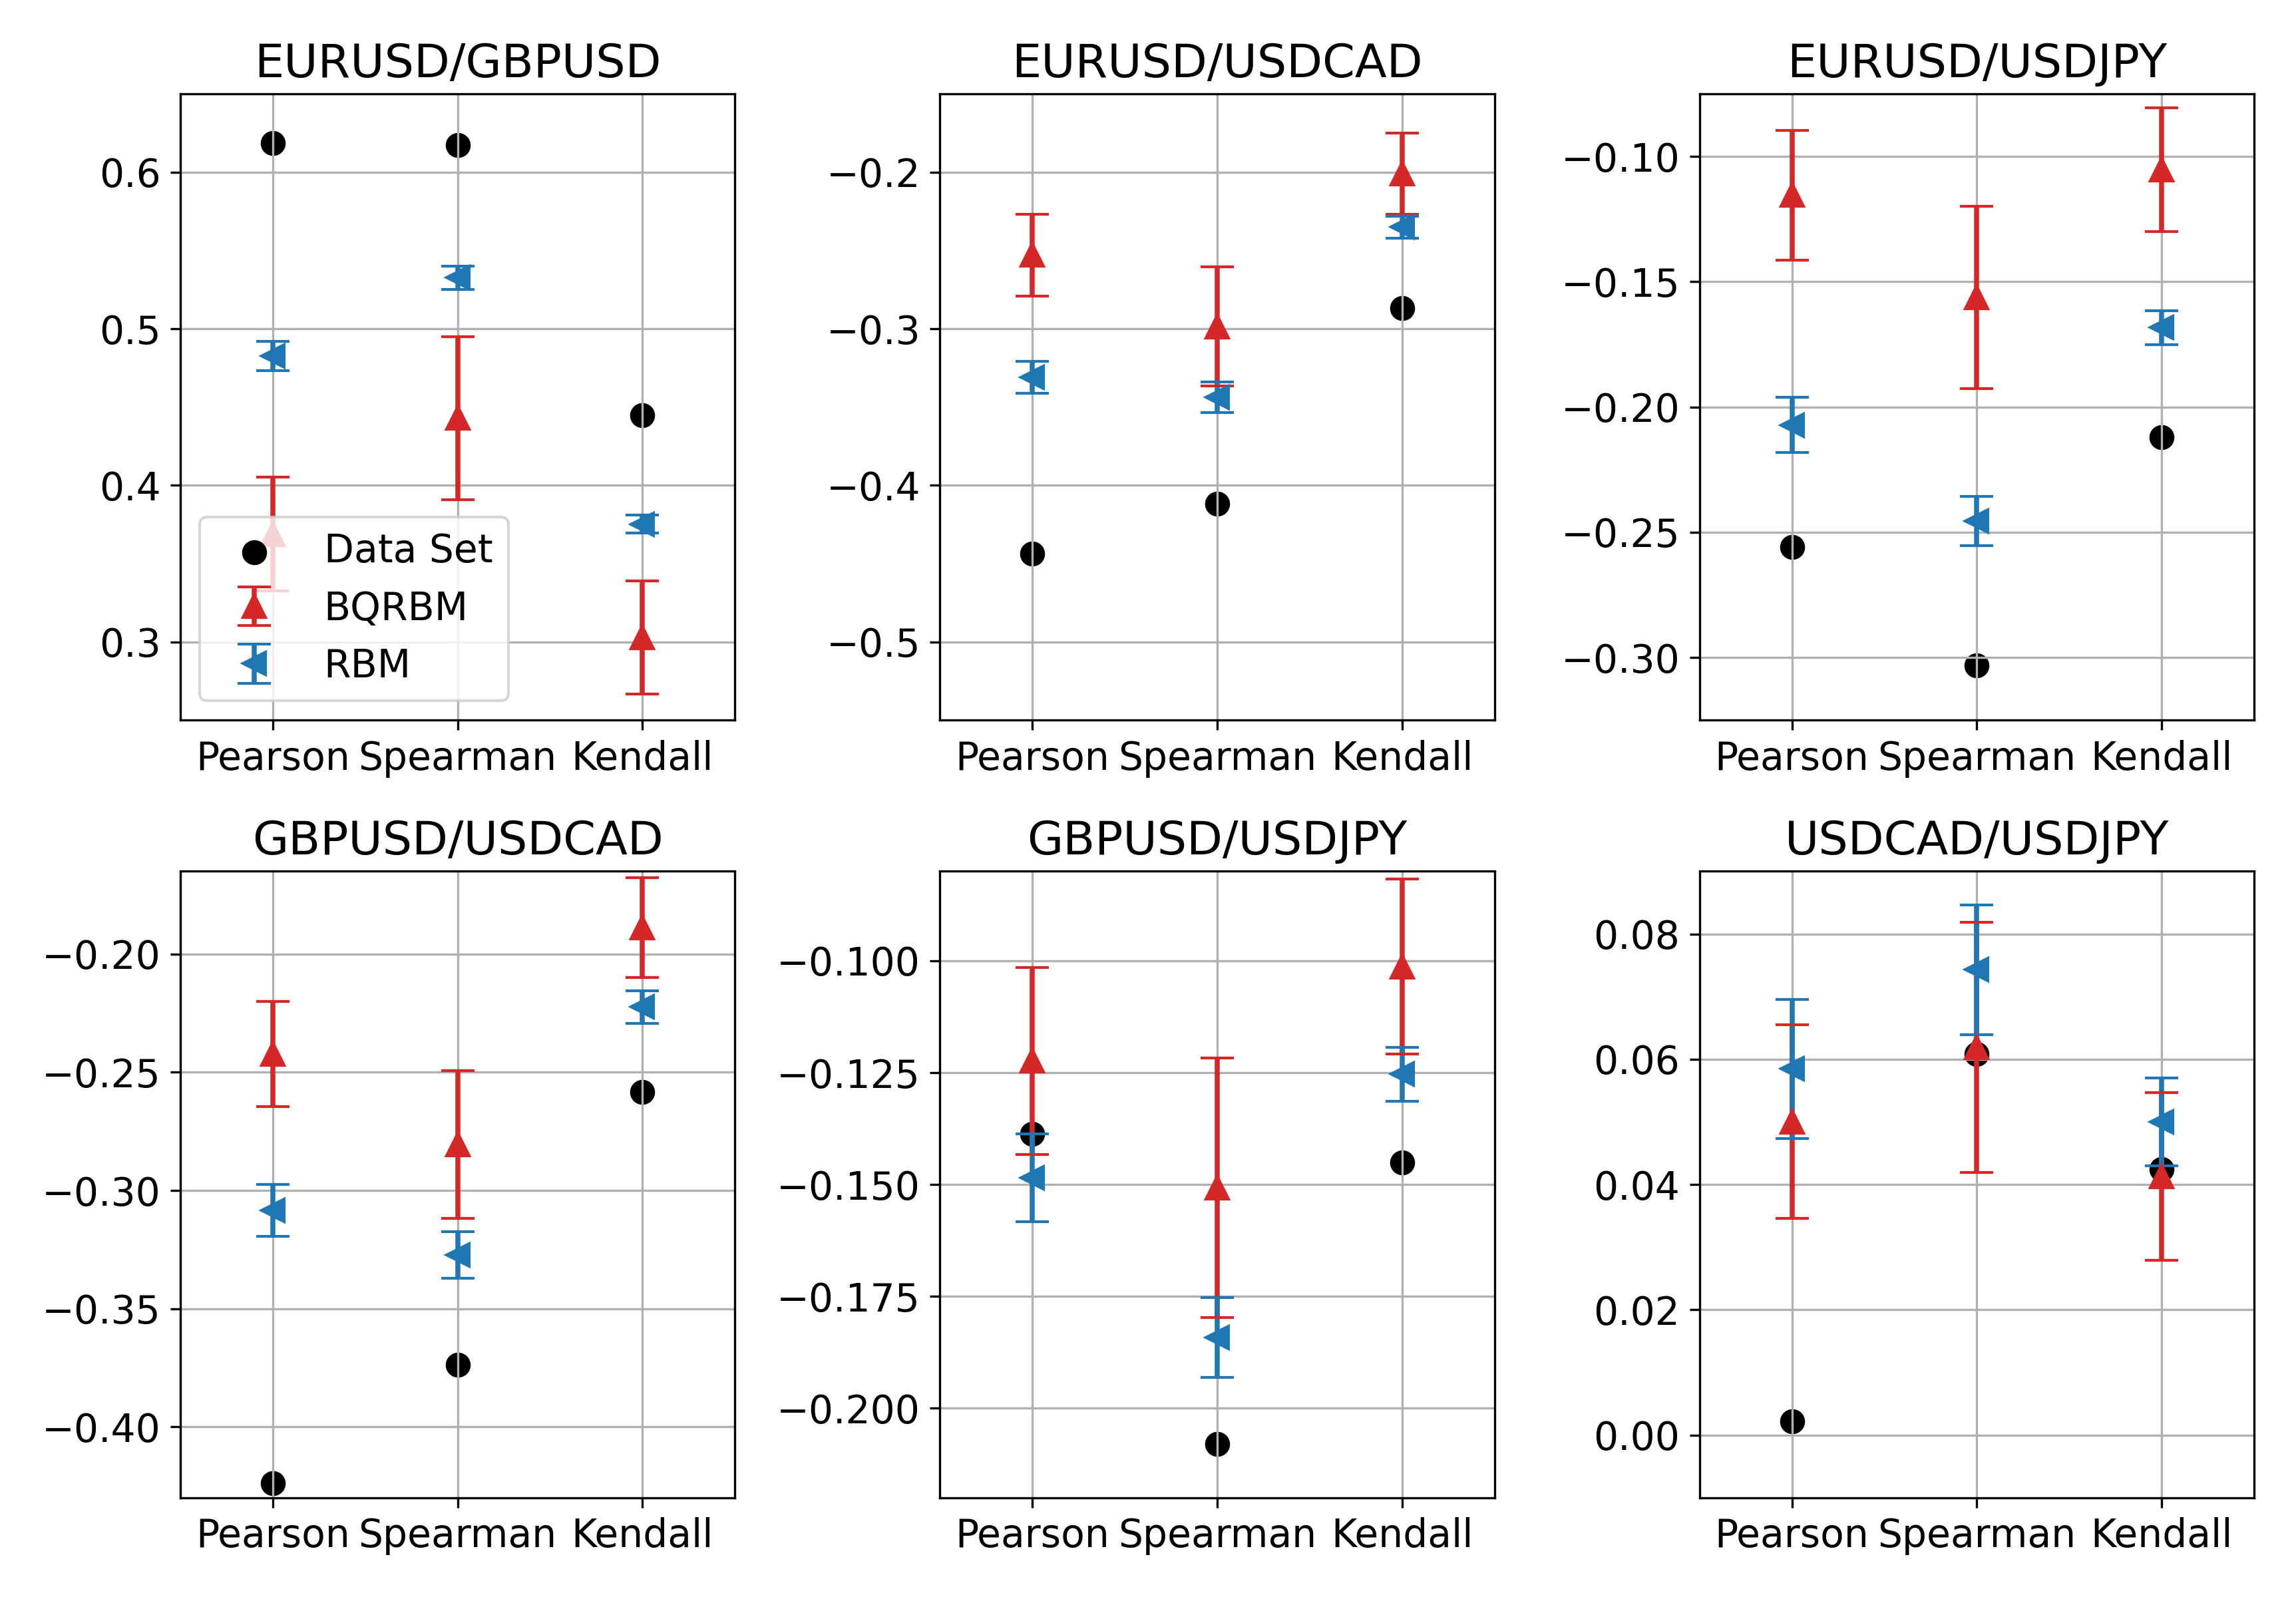
\includegraphics[width=0.9\linewidth]{qbm/log_returns/correlation_coefficients.png}
    \end{figure}
\end{frame}

\begin{frame}
    \frametitle{Volatilities}
    \begin{table}[!htb]
        \centering
        \begin{adjustbox}{max width=\textwidth}
            \input{../../tables/qbm/volatilities.tbl}
        \end{adjustbox}
    \end{table}
\end{frame}

\begin{frame}
    \frametitle{Tails}
    \begin{table}[!htb]
        \centering
        \begin{adjustbox}{max height=35mm}
            \input{../../tables/qbm/tails.tbl}
        \end{adjustbox}
    \end{table}
\end{frame}

\begin{frame}
    \frametitle{QQ Plots}
    \begin{figure}
        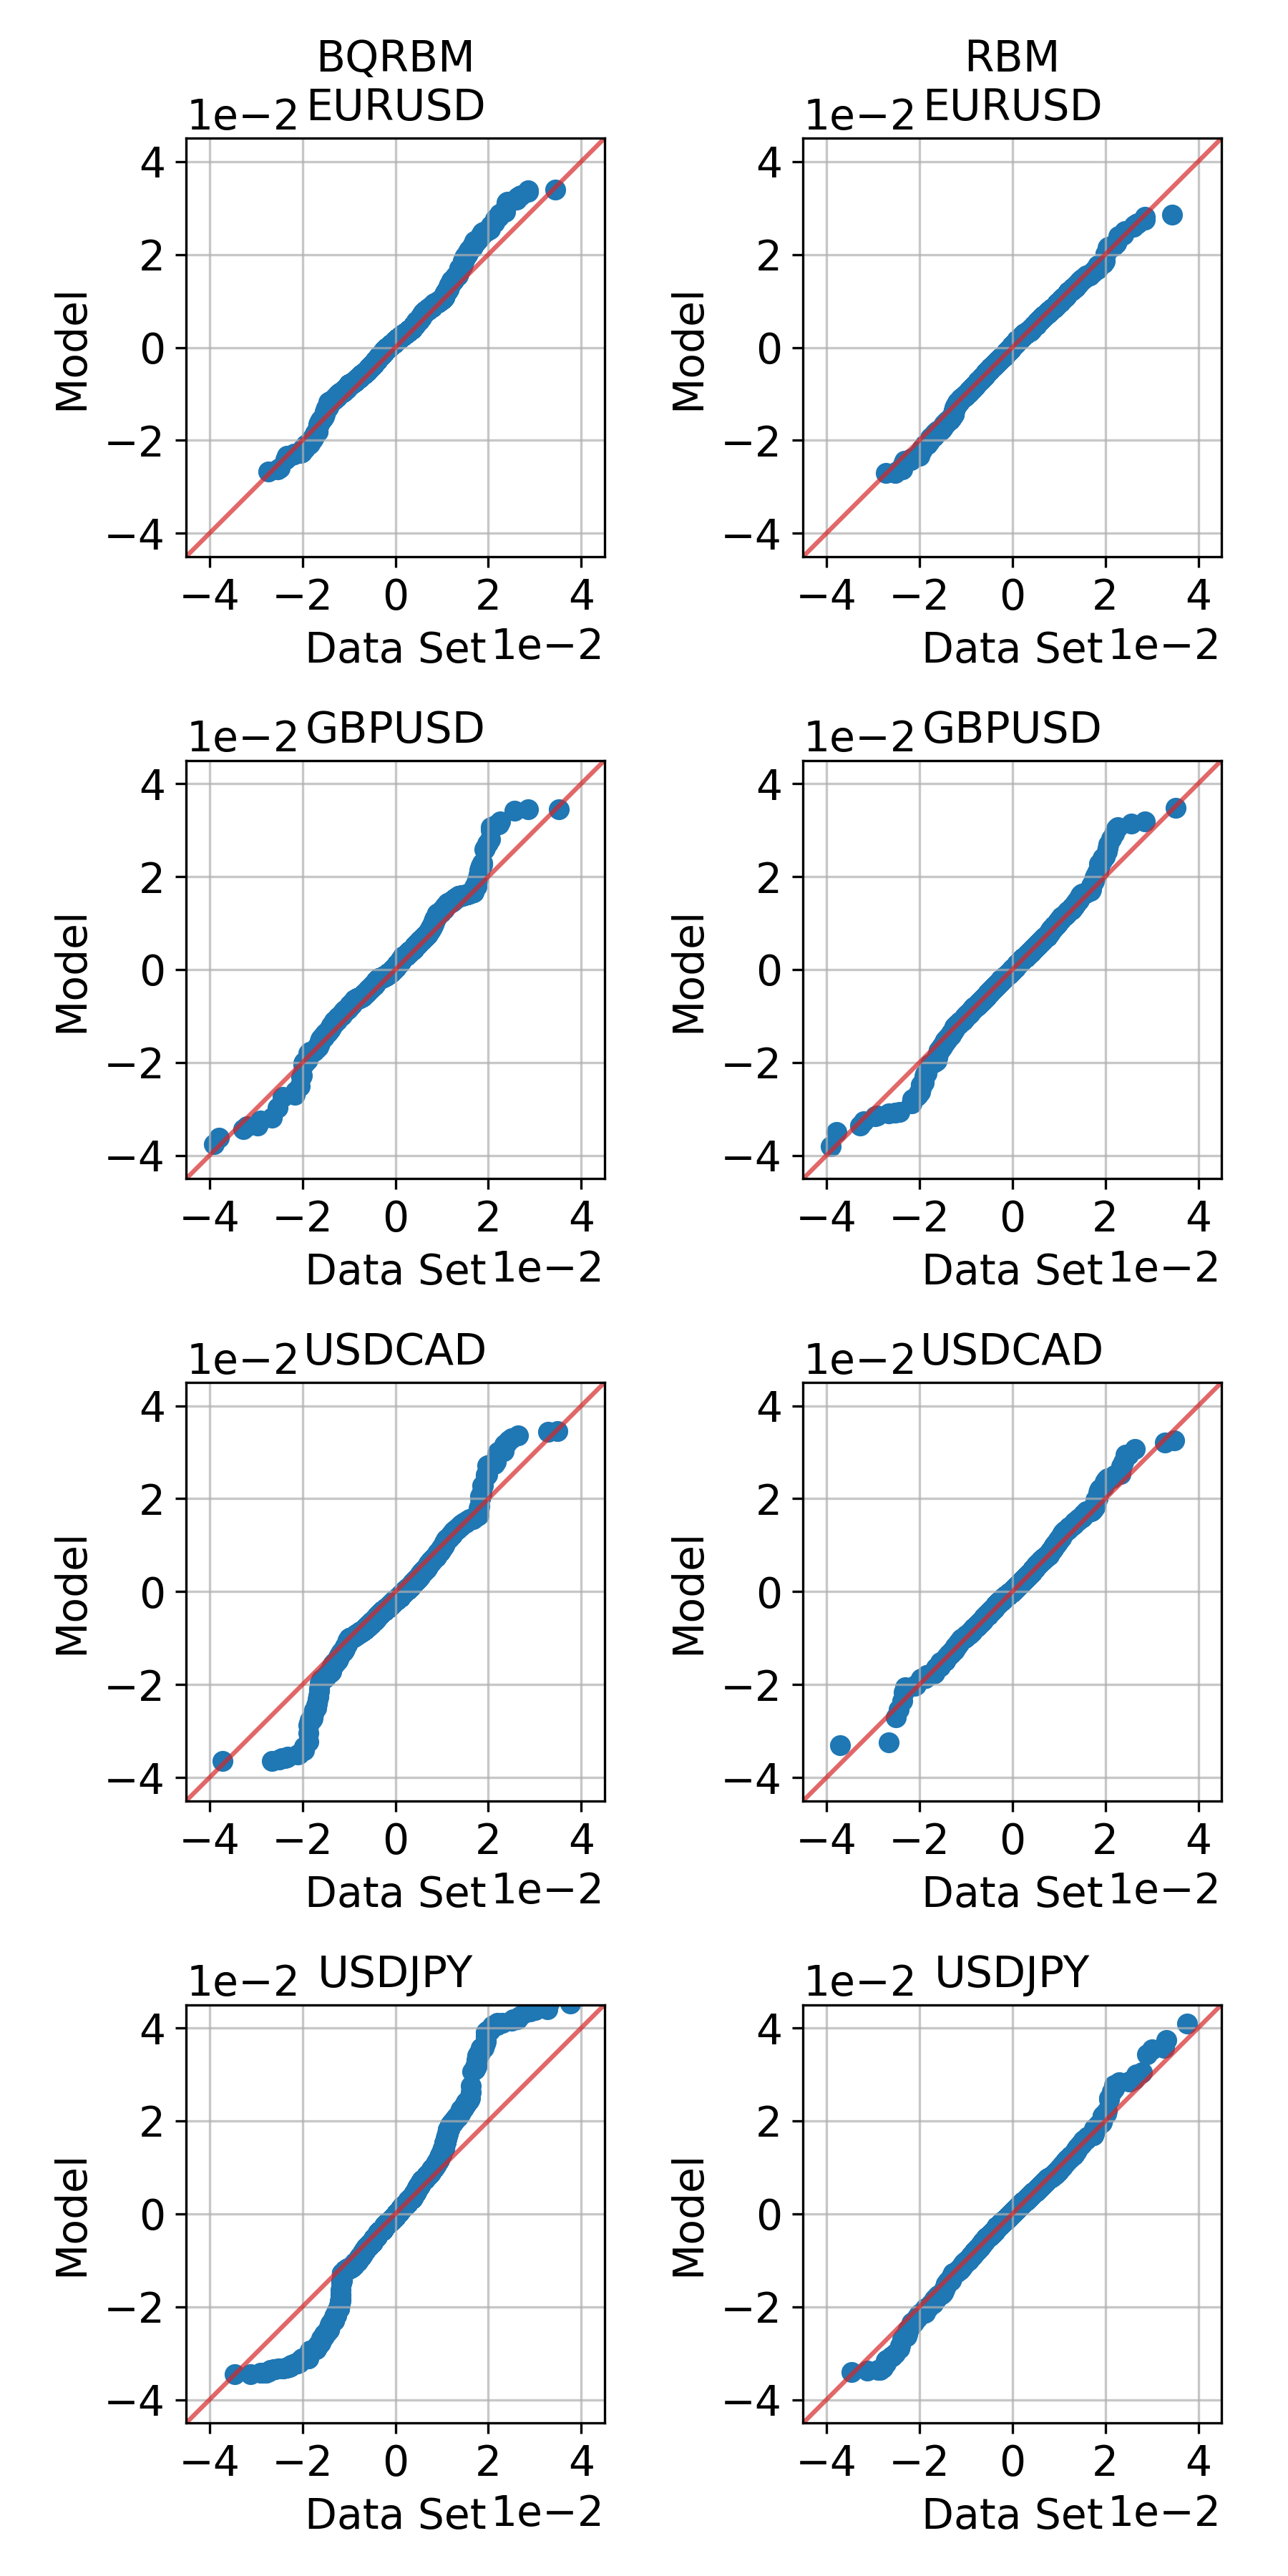
\includegraphics[width=0.3\linewidth]{qbm/log_returns/qq.png}
    \end{figure}
\end{frame}

%----------------------------------------------------------------------------------------
% References and Resources
%----------------------------------------------------------------------------------------

\section{References and Resources}

\begin{frame}[allowframebreaks]
    \frametitle{References}
    \footnotesize{
        \bibliographystyle{abbrv}
        \bibliography{../../references.bib}
    }
\end{frame}

\end{document}
